% Options for packages loaded elsewhere
\PassOptionsToPackage{unicode}{hyperref}
\PassOptionsToPackage{hyphens}{url}
%
\documentclass[
]{article}
\usepackage{amsmath,amssymb}
\usepackage{iftex}
\ifPDFTeX
  \usepackage[T1]{fontenc}
  \usepackage[utf8]{inputenc}
  \usepackage{textcomp} % provide euro and other symbols
\else % if luatex or xetex
  \usepackage{unicode-math} % this also loads fontspec
  \defaultfontfeatures{Scale=MatchLowercase}
  \defaultfontfeatures[\rmfamily]{Ligatures=TeX,Scale=1}
\fi
\usepackage{lmodern}
\ifPDFTeX\else
  % xetex/luatex font selection
\fi
% Use upquote if available, for straight quotes in verbatim environments
\IfFileExists{upquote.sty}{\usepackage{upquote}}{}
\IfFileExists{microtype.sty}{% use microtype if available
  \usepackage[]{microtype}
  \UseMicrotypeSet[protrusion]{basicmath} % disable protrusion for tt fonts
}{}
\makeatletter
\@ifundefined{KOMAClassName}{% if non-KOMA class
  \IfFileExists{parskip.sty}{%
    \usepackage{parskip}
  }{% else
    \setlength{\parindent}{0pt}
    \setlength{\parskip}{6pt plus 2pt minus 1pt}}
}{% if KOMA class
  \KOMAoptions{parskip=half}}
\makeatother
\usepackage{xcolor}
\usepackage[margin=1in]{geometry}
\usepackage{color}
\usepackage{fancyvrb}
\newcommand{\VerbBar}{|}
\newcommand{\VERB}{\Verb[commandchars=\\\{\}]}
\DefineVerbatimEnvironment{Highlighting}{Verbatim}{commandchars=\\\{\}}
% Add ',fontsize=\small' for more characters per line
\usepackage{framed}
\definecolor{shadecolor}{RGB}{248,248,248}
\newenvironment{Shaded}{\begin{snugshade}}{\end{snugshade}}
\newcommand{\AlertTok}[1]{\textcolor[rgb]{0.94,0.16,0.16}{#1}}
\newcommand{\AnnotationTok}[1]{\textcolor[rgb]{0.56,0.35,0.01}{\textbf{\textit{#1}}}}
\newcommand{\AttributeTok}[1]{\textcolor[rgb]{0.13,0.29,0.53}{#1}}
\newcommand{\BaseNTok}[1]{\textcolor[rgb]{0.00,0.00,0.81}{#1}}
\newcommand{\BuiltInTok}[1]{#1}
\newcommand{\CharTok}[1]{\textcolor[rgb]{0.31,0.60,0.02}{#1}}
\newcommand{\CommentTok}[1]{\textcolor[rgb]{0.56,0.35,0.01}{\textit{#1}}}
\newcommand{\CommentVarTok}[1]{\textcolor[rgb]{0.56,0.35,0.01}{\textbf{\textit{#1}}}}
\newcommand{\ConstantTok}[1]{\textcolor[rgb]{0.56,0.35,0.01}{#1}}
\newcommand{\ControlFlowTok}[1]{\textcolor[rgb]{0.13,0.29,0.53}{\textbf{#1}}}
\newcommand{\DataTypeTok}[1]{\textcolor[rgb]{0.13,0.29,0.53}{#1}}
\newcommand{\DecValTok}[1]{\textcolor[rgb]{0.00,0.00,0.81}{#1}}
\newcommand{\DocumentationTok}[1]{\textcolor[rgb]{0.56,0.35,0.01}{\textbf{\textit{#1}}}}
\newcommand{\ErrorTok}[1]{\textcolor[rgb]{0.64,0.00,0.00}{\textbf{#1}}}
\newcommand{\ExtensionTok}[1]{#1}
\newcommand{\FloatTok}[1]{\textcolor[rgb]{0.00,0.00,0.81}{#1}}
\newcommand{\FunctionTok}[1]{\textcolor[rgb]{0.13,0.29,0.53}{\textbf{#1}}}
\newcommand{\ImportTok}[1]{#1}
\newcommand{\InformationTok}[1]{\textcolor[rgb]{0.56,0.35,0.01}{\textbf{\textit{#1}}}}
\newcommand{\KeywordTok}[1]{\textcolor[rgb]{0.13,0.29,0.53}{\textbf{#1}}}
\newcommand{\NormalTok}[1]{#1}
\newcommand{\OperatorTok}[1]{\textcolor[rgb]{0.81,0.36,0.00}{\textbf{#1}}}
\newcommand{\OtherTok}[1]{\textcolor[rgb]{0.56,0.35,0.01}{#1}}
\newcommand{\PreprocessorTok}[1]{\textcolor[rgb]{0.56,0.35,0.01}{\textit{#1}}}
\newcommand{\RegionMarkerTok}[1]{#1}
\newcommand{\SpecialCharTok}[1]{\textcolor[rgb]{0.81,0.36,0.00}{\textbf{#1}}}
\newcommand{\SpecialStringTok}[1]{\textcolor[rgb]{0.31,0.60,0.02}{#1}}
\newcommand{\StringTok}[1]{\textcolor[rgb]{0.31,0.60,0.02}{#1}}
\newcommand{\VariableTok}[1]{\textcolor[rgb]{0.00,0.00,0.00}{#1}}
\newcommand{\VerbatimStringTok}[1]{\textcolor[rgb]{0.31,0.60,0.02}{#1}}
\newcommand{\WarningTok}[1]{\textcolor[rgb]{0.56,0.35,0.01}{\textbf{\textit{#1}}}}
\usepackage{longtable,booktabs,array}
\usepackage{calc} % for calculating minipage widths
% Correct order of tables after \paragraph or \subparagraph
\usepackage{etoolbox}
\makeatletter
\patchcmd\longtable{\par}{\if@noskipsec\mbox{}\fi\par}{}{}
\makeatother
% Allow footnotes in longtable head/foot
\IfFileExists{footnotehyper.sty}{\usepackage{footnotehyper}}{\usepackage{footnote}}
\makesavenoteenv{longtable}
\usepackage{graphicx}
\makeatletter
\def\maxwidth{\ifdim\Gin@nat@width>\linewidth\linewidth\else\Gin@nat@width\fi}
\def\maxheight{\ifdim\Gin@nat@height>\textheight\textheight\else\Gin@nat@height\fi}
\makeatother
% Scale images if necessary, so that they will not overflow the page
% margins by default, and it is still possible to overwrite the defaults
% using explicit options in \includegraphics[width, height, ...]{}
\setkeys{Gin}{width=\maxwidth,height=\maxheight,keepaspectratio}
% Set default figure placement to htbp
\makeatletter
\def\fps@figure{htbp}
\makeatother
\setlength{\emergencystretch}{3em} % prevent overfull lines
\providecommand{\tightlist}{%
  \setlength{\itemsep}{0pt}\setlength{\parskip}{0pt}}
\setcounter{secnumdepth}{5}
\usepackage{float}
\ifLuaTeX
  \usepackage{selnolig}  % disable illegal ligatures
\fi
\usepackage[]{natbib}
\bibliographystyle{plainnat}
\usepackage{bookmark}
\IfFileExists{xurl.sty}{\usepackage{xurl}}{} % add URL line breaks if available
\urlstyle{same}
\hypersetup{
  pdftitle={Introduction to SLGP Package},
  pdfauthor={Athénaïs Gautier},
  hidelinks,
  pdfcreator={LaTeX via pandoc}}

\title{Introduction to SLGP Package}
\author{Athénaïs Gautier}
\date{}

\begin{document}
\maketitle

This vignette provides a practical introduction to Spatial Logistic Gaussian Process (SLGP) modeling, demonstrating its implementation and application..

\section{Dataset}\label{dataset}

We illustrate the model's capabilities using the Boston Housing dataset \citet{harrison_hedonic_1978}, a well-known benchmark in statistical modeling and regression analysis.

For this vignette, we focus on modeling the distribution of median home values (\texttt{medv}) as a function of the proportion of pre-1940 owner-occupied units (\texttt{age}). This example highlights the ability of SLGPs to capture complex, spatially dependent distributions in data that exhibit heterogeneity and multi-modality.

\begin{Shaded}
\begin{Highlighting}[]
\FunctionTok{library}\NormalTok{(dplyr)}
\CommentTok{\# Load the dataset (available in MASS package)}
\ControlFlowTok{if}\NormalTok{ (}\SpecialCharTok{!}\FunctionTok{requireNamespace}\NormalTok{(}\StringTok{"MASS"}\NormalTok{, }\AttributeTok{quietly =} \ConstantTok{TRUE}\NormalTok{)) }\FunctionTok{install.packages}\NormalTok{(}\StringTok{"MASS"}\NormalTok{)}
\FunctionTok{data}\NormalTok{(}\StringTok{"Boston"}\NormalTok{, }\AttributeTok{package =} \StringTok{"MASS"}\NormalTok{)}
\NormalTok{df }\OtherTok{\textless{}{-}}\NormalTok{ Boston }\SpecialCharTok{\%\textgreater{}\%}
  \FunctionTok{mutate}\NormalTok{(}\AttributeTok{age\_bin =} \FunctionTok{cut}\NormalTok{(age, }\AttributeTok{breaks =} \FunctionTok{seq}\NormalTok{(}\DecValTok{0}\NormalTok{, }\DecValTok{100}\NormalTok{, }\AttributeTok{by =} \DecValTok{10}\NormalTok{), }\AttributeTok{include.lowest =} \ConstantTok{FALSE}\NormalTok{)) }\SpecialCharTok{\%\textgreater{}\%}
  \FunctionTok{group\_by}\NormalTok{(age\_bin) }\SpecialCharTok{\%\textgreater{}\%}
  \FunctionTok{mutate}\NormalTok{(}\AttributeTok{age\_bin =} \FunctionTok{paste0}\NormalTok{(age\_bin, }\StringTok{"}\SpecialCharTok{\textbackslash{}n}\StringTok{n="}\NormalTok{, }\FunctionTok{n}\NormalTok{()))}\SpecialCharTok{\%\textgreater{}\%}
  \FunctionTok{ungroup}\NormalTok{()}\SpecialCharTok{\%\textgreater{}\%}
  \FunctionTok{mutate}\NormalTok{(}\AttributeTok{age\_bin =} \FunctionTok{factor}\NormalTok{(age\_bin, }
                          \AttributeTok{levels =} \FunctionTok{sort}\NormalTok{(}\FunctionTok{unique}\NormalTok{(age\_bin), }\AttributeTok{decreasing =} \ConstantTok{FALSE}\NormalTok{))) }\SpecialCharTok{\%\textgreater{}\%}
  \FunctionTok{data.frame}\NormalTok{()}

\NormalTok{range\_response }\OtherTok{\textless{}{-}} \FunctionTok{c}\NormalTok{(}\DecValTok{0}\NormalTok{, }\DecValTok{50}\NormalTok{) }\CommentTok{\# Can use range(df$medv), or user defined range as we do here}
\NormalTok{range\_x }\OtherTok{\textless{}{-}} \FunctionTok{c}\NormalTok{(}\DecValTok{0}\NormalTok{, }\DecValTok{100}\NormalTok{) }\CommentTok{\# Can use range(df$age), or user defined range as we do here}
\end{Highlighting}
\end{Shaded}

We represent the data to visualise the relationship between \texttt{medv} and \texttt{age}.

\begin{Shaded}
\begin{Highlighting}[]
\FunctionTok{library}\NormalTok{(ggplot2)}
\FunctionTok{library}\NormalTok{(ggpubr)}
\CommentTok{\#\textgreater{} Warning: le package \textquotesingle{}ggpubr\textquotesingle{} a été compilé avec la version R 4.4.2}
\FunctionTok{library}\NormalTok{(viridis)}
\CommentTok{\#\textgreater{} Le chargement a nécessité le package : viridisLite}
\CommentTok{\# Scatterplot: med vs. age}
\NormalTok{scatter\_plot }\OtherTok{\textless{}{-}} \FunctionTok{ggplot}\NormalTok{(df, }\FunctionTok{aes}\NormalTok{(}\AttributeTok{x =}\NormalTok{ age, }\AttributeTok{y =}\NormalTok{ medv)) }\SpecialCharTok{+}
  \FunctionTok{geom\_point}\NormalTok{(}\AttributeTok{alpha =} \FloatTok{0.5}\NormalTok{, }\AttributeTok{color =} \StringTok{"navy"}\NormalTok{) }\SpecialCharTok{+}
  \FunctionTok{labs}\NormalTok{(}\AttributeTok{x =} \StringTok{"Proportion of owner{-}occupied units}\SpecialCharTok{\textbackslash{}n}\StringTok{built prior to 1940 [AGE, \%]"}\NormalTok{, }
       \AttributeTok{y =} \StringTok{"Median value of owner{-}occupied homes [MEDV, k$]"}\NormalTok{,}
       \AttributeTok{title =} \StringTok{"Median value vs. age of homes"}\NormalTok{) }\SpecialCharTok{+}
  \FunctionTok{theme\_bw}\NormalTok{()}\SpecialCharTok{+}
  \FunctionTok{coord\_cartesian}\NormalTok{(}\AttributeTok{xlim=}\NormalTok{range\_x,}
                  \AttributeTok{ylim=}\NormalTok{range\_response)}

\CommentTok{\# Histogram: Distribution of med by age bin}
\NormalTok{hist\_plot }\OtherTok{\textless{}{-}} \FunctionTok{ggplot}\NormalTok{(df, }\FunctionTok{aes}\NormalTok{(}\AttributeTok{x =}\NormalTok{ medv)) }\SpecialCharTok{+}
  \FunctionTok{geom\_histogram}\NormalTok{(}\AttributeTok{mapping=}\FunctionTok{aes}\NormalTok{(}\AttributeTok{y=}\FunctionTok{after\_stat}\NormalTok{(density)),}
                 \AttributeTok{position =} \StringTok{"identity"}\NormalTok{, }\AttributeTok{breaks =} \FunctionTok{seq}\NormalTok{(}\DecValTok{0}\NormalTok{, }\DecValTok{50}\NormalTok{, }\FloatTok{2.5}\NormalTok{),}
                 \AttributeTok{fill=}\StringTok{"darkgrey"}\NormalTok{, }\AttributeTok{col=}\StringTok{"grey50"}\NormalTok{, }\AttributeTok{lwd=}\FloatTok{0.2}\NormalTok{, }\AttributeTok{alpha=}\FloatTok{0.7}\NormalTok{) }\SpecialCharTok{+}
  \FunctionTok{geom\_rug}\NormalTok{(}\AttributeTok{sides =} \StringTok{"b"}\NormalTok{, }\AttributeTok{color =} \StringTok{"navy"}\NormalTok{, }\AttributeTok{alpha =} \FloatTok{0.5}\NormalTok{)}\SpecialCharTok{+}
  \FunctionTok{facet\_wrap}\NormalTok{(}\SpecialCharTok{\textasciitilde{}}\NormalTok{ age\_bin, }\AttributeTok{scales =} \StringTok{"free\_y"}\NormalTok{, }\AttributeTok{nrow=}\DecValTok{2}\NormalTok{) }\SpecialCharTok{+}
  \FunctionTok{labs}\NormalTok{(}\AttributeTok{x =} \StringTok{"Median value of owner{-}occupied homes [MEDV, k$]"}\NormalTok{, }
       \AttributeTok{y =} \StringTok{"Probability density"}\NormalTok{, }
       \AttributeTok{title =} \StringTok{"Histogram of median housing values by AGE group"}\NormalTok{) }\SpecialCharTok{+}
  \FunctionTok{theme\_bw}\NormalTok{()}\SpecialCharTok{+}
  \FunctionTok{coord\_cartesian}\NormalTok{(}\AttributeTok{xlim=}\NormalTok{range\_response,}
                  \AttributeTok{ylim=}\FunctionTok{c}\NormalTok{(}\DecValTok{0}\NormalTok{, }\FloatTok{0.25}\NormalTok{))}
\FunctionTok{ggarrange}\NormalTok{(scatter\_plot, hist\_plot, }\AttributeTok{ncol =} \DecValTok{2}\NormalTok{, }\AttributeTok{nrow =} \DecValTok{1}\NormalTok{,}
          \AttributeTok{widths =} \FunctionTok{c}\NormalTok{(}\FloatTok{0.3}\NormalTok{, }\FloatTok{0.7}\NormalTok{))}
\end{Highlighting}
\end{Shaded}

\begin{figure}[H]

{\centering 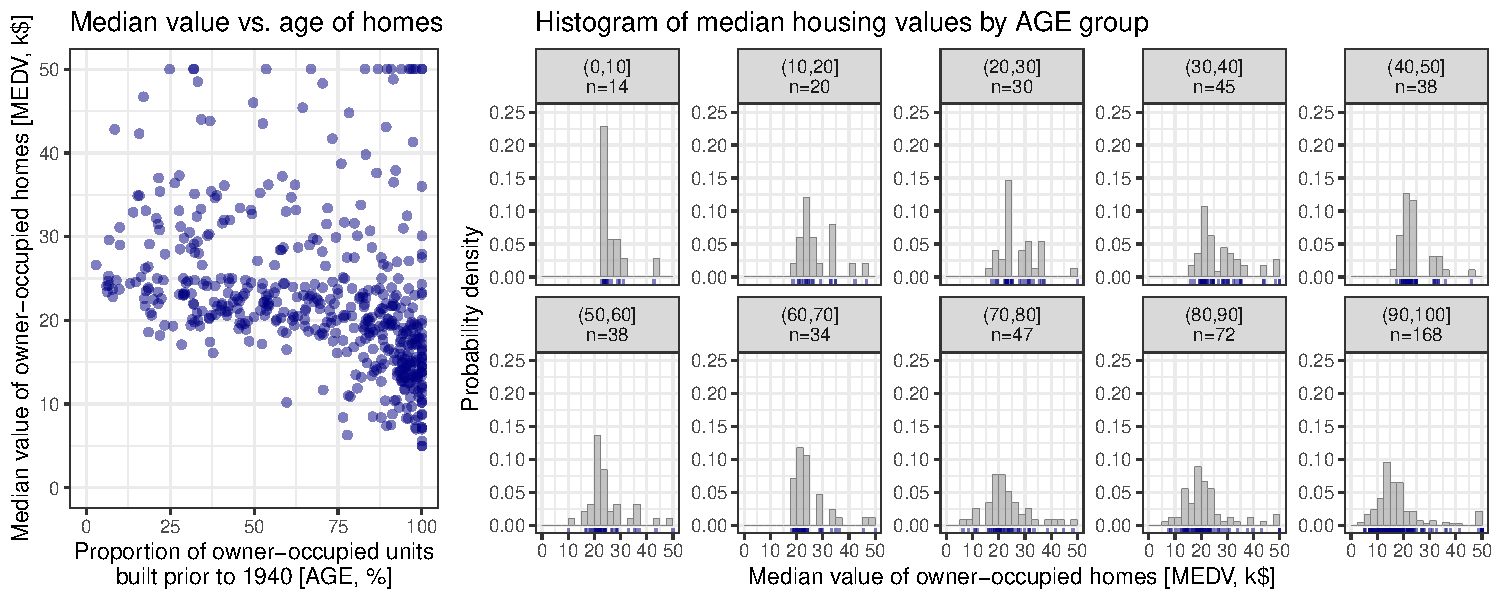
\includegraphics{IntroductionSLGP_files/figure-latex/figureHousing-1} 

}

\caption{A visual representation of the dependency of the median value of owner-occupied homes on proportion of owner-occupied units constructed before 1940 in the Boston Housing dataset.}\label{fig:figureHousing}
\end{figure}

\begin{Shaded}
\begin{Highlighting}[]
\FunctionTok{ggsave}\NormalTok{(}\StringTok{"./Figures/scatter.pdf"}\NormalTok{, }\AttributeTok{width=}\DecValTok{10}\NormalTok{, }\AttributeTok{height=}\FloatTok{3.5}\NormalTok{)}
\end{Highlighting}
\end{Shaded}

We see that there is a general trend where older homes tend to have lower values, with exceptions likely due to survivor bias: older homes that persist tend to be of higher structural quality. This dataset provides an test case for SLGP modeling, offering a compact, one-dimensional covariate space, heterogeneously distributed data, and shifting distributional shapes.

\section{SLGP model specifications}\label{slgp-model-specifications}

To model the distributional changes observed in the Boston Housing dataset, we now introduce the Spatial Logistic Gaussian Process (SLGP) model. SLGPs provide a flexible non-parametric framework for modeling spatially dependent probability densities. By transforming a Gaussian Process (GP) through exponentiation and normalization, SLGPs ensure positivity and integration to one, making them well-suited for density estimation.
In this section, we specify the SLGP prior, and visualise its behaviour.

\subsection{Prior}\label{prior}

The prior in an SLGP represents our initial beliefs about the structure of the data before incorporating observations. It defines a distribution over possible density functions, capturing spatial dependencies while allowing sufficient flexibility.
The following code chunk sets up an SLGP prior over \texttt{medv\ \textasciitilde{}\ age}, where \texttt{medv} is modeled as a function of \texttt{age}:

\begin{Shaded}
\begin{Highlighting}[]
\FunctionTok{library}\NormalTok{(SLGP)}

\NormalTok{modelPrior }\OtherTok{\textless{}{-}} \FunctionTok{slgp}\NormalTok{(medv}\SpecialCharTok{\textasciitilde{}}\NormalTok{age, }\CommentTok{\# Use a formula to specify predictors VS response}
                   \CommentTok{\# Can use medv\textasciitilde{}. for all variables,}
                   \CommentTok{\# Or medv \textasciitilde{} age + var2 + var3 for more variables}
                   \AttributeTok{data=}\NormalTok{df,}
                   \AttributeTok{method=}\StringTok{"none"}\NormalTok{, }\CommentTok{\#Maximum a posteriori estimation scheme}
                   \AttributeTok{basisFunctionsUsed =} \StringTok{"RFF"}\NormalTok{,}
                   \AttributeTok{interpolateBasisFun=}\StringTok{"WNN"}\NormalTok{, }\CommentTok{\# Will Accelerate inference}
                   \AttributeTok{hyperparams =} \FunctionTok{list}\NormalTok{(}\AttributeTok{lengthscale=}\FunctionTok{c}\NormalTok{(}\FloatTok{0.15}\NormalTok{, }\FloatTok{0.15}\NormalTok{), }
                                      \CommentTok{\# Applied to normalised data}
                                      \CommentTok{\# So 0.15 is 15\% of the range of values}
                                      \AttributeTok{sigma2=}\DecValTok{1}\NormalTok{), }
                   \CommentTok{\# Will be re{-}selected with sigmaEstimationMethod}
                   \AttributeTok{sigmaEstimationMethod =} \StringTok{"heuristic"}\NormalTok{, }
                   \CommentTok{\# Set to heuristic for numerical stability                 }
                   \AttributeTok{predictorsLower=} \FunctionTok{c}\NormalTok{(range\_x[}\DecValTok{1}\NormalTok{]),}
                   \AttributeTok{predictorsUpper=} \FunctionTok{c}\NormalTok{(range\_x[}\DecValTok{2}\NormalTok{]),}
                   \AttributeTok{responseRange=}\NormalTok{ range\_response,}
                   \AttributeTok{opts\_BasisFun =} \FunctionTok{list}\NormalTok{(}\AttributeTok{nFreq=}\DecValTok{200}\NormalTok{,}
                                        \AttributeTok{MatParam=}\DecValTok{5}\SpecialCharTok{/}\DecValTok{2}\NormalTok{),}
                   \AttributeTok{seed=}\DecValTok{1}\NormalTok{)}
\end{Highlighting}
\end{Shaded}

Here:

\begin{itemize}
\item
  The model uses Random Fourier Features (RFF) for the finite-rank latent GP.
\item
  The lengthscale (15\% of the normalized range) controls the smoothness of variation. This is selected following our proposed heuristic.
\item
  The heuristic sigma estimation ensures numerical stability.
\end{itemize}

\subsubsection{Looking at several draws of the prior}\label{looking-at-several-draws-of-the-prior}

To understand how the SLGP prior behaves, we generate and visualize random draws from the prior distribution over probability densities of \texttt{medv} at different \texttt{age} values.

\begin{Shaded}
\begin{Highlighting}[]


\FunctionTok{library}\NormalTok{(tidyr)}
\NormalTok{nrep }\OtherTok{\textless{}{-}} \DecValTok{3}
\FunctionTok{set.seed}\NormalTok{(}\DecValTok{8}\NormalTok{)}
\NormalTok{p }\OtherTok{\textless{}{-}} \FunctionTok{ncol}\NormalTok{(modelPrior}\SpecialCharTok{@}\NormalTok{coefficients)}
\NormalTok{modelPrior}\SpecialCharTok{@}\NormalTok{coefficients }\OtherTok{\textless{}{-}} \FunctionTok{matrix}\NormalTok{(}\FunctionTok{rnorm}\NormalTok{(}\AttributeTok{n=}\NormalTok{nrep}\SpecialCharTok{*}\NormalTok{p), }\AttributeTok{nrow=}\NormalTok{nrep)}

\NormalTok{dfGrid }\OtherTok{\textless{}{-}} \FunctionTok{data.frame}\NormalTok{(}\FunctionTok{expand.grid}\NormalTok{(}\FunctionTok{seq}\NormalTok{(range\_x[}\DecValTok{1}\NormalTok{], range\_x[}\DecValTok{2}\NormalTok{], }\DecValTok{5}\NormalTok{), }
                                 \FunctionTok{seq}\NormalTok{(range\_response[}\DecValTok{1}\NormalTok{], range\_response[}\DecValTok{2}\NormalTok{],, }\DecValTok{101}\NormalTok{)))}
\FunctionTok{colnames}\NormalTok{(dfGrid) }\OtherTok{\textless{}{-}} \FunctionTok{c}\NormalTok{(}\StringTok{"age"}\NormalTok{, }\StringTok{"medv"}\NormalTok{)}
\NormalTok{predPrior }\OtherTok{\textless{}{-}} \FunctionTok{predictSLGP\_newNode}\NormalTok{(}\AttributeTok{SLGPmodel=}\NormalTok{modelPrior,}
                                 \AttributeTok{newNodes =}\NormalTok{ dfGrid)}
\FunctionTok{colnames}\NormalTok{(predPrior) }\OtherTok{\textless{}{-}} \FunctionTok{c}\NormalTok{(}\StringTok{"age"}\NormalTok{, }\StringTok{"medv"}\NormalTok{, }\FunctionTok{paste0}\NormalTok{(}\StringTok{"Draw from the prior n°"}\NormalTok{, }\FunctionTok{seq}\NormalTok{(nrep)))}
\NormalTok{predPrior }\OtherTok{\textless{}{-}}\NormalTok{ predPrior}\SpecialCharTok{\%\textgreater{}\%}
  \FunctionTok{pivot\_longer}\NormalTok{(}\SpecialCharTok{{-}}\FunctionTok{c}\NormalTok{(}\StringTok{"age"}\NormalTok{, }\StringTok{"medv"}\NormalTok{))}
\NormalTok{scale\_factor }\OtherTok{\textless{}{-}} \DecValTok{200}
\FunctionTok{ggplot}\NormalTok{()  }\SpecialCharTok{+}
  \FunctionTok{labs}\NormalTok{(}\AttributeTok{y =} \StringTok{"Proportion of owner{-}occupied units built prior to 1940 [AGE, \%]"}\NormalTok{, }
       \AttributeTok{x =} \StringTok{"Median value of owner{-}occupied homes [MEDV, k$]"}\NormalTok{,}
       \AttributeTok{title =} \StringTok{"Samples from the SLGP Prior for the pdfs of MEDV at AGE, }
\StringTok{       visualised across slices"}\NormalTok{) }\SpecialCharTok{+}
  \FunctionTok{theme\_bw}\NormalTok{()}\SpecialCharTok{+}
  \FunctionTok{geom\_ribbon}\NormalTok{(}\AttributeTok{data=}\NormalTok{predPrior,}
              \AttributeTok{mapping=}\FunctionTok{aes}\NormalTok{(}\AttributeTok{x=}\NormalTok{medv, }\AttributeTok{ymax=}\NormalTok{scale\_factor}\SpecialCharTok{*}\NormalTok{value}\SpecialCharTok{+}\NormalTok{age, }
                          \AttributeTok{ymin=}\NormalTok{age, }\AttributeTok{group=}\SpecialCharTok{{-}}\NormalTok{age, }\AttributeTok{fill=}\NormalTok{age),}
              \AttributeTok{col=}\StringTok{"grey"}\NormalTok{, }\AttributeTok{alpha=}\FloatTok{0.9}\NormalTok{)}\SpecialCharTok{+}
  \CommentTok{\# geom\_point(data=df,}
  \CommentTok{\#            mapping=aes(x = medv, y = age), alpha = 0.5, color = "navy")+}
  \FunctionTok{scale\_fill\_viridis}\NormalTok{(}\AttributeTok{option =} \StringTok{"plasma"}\NormalTok{,}
                     \AttributeTok{guide =} \FunctionTok{guide\_colorbar}\NormalTok{(}\AttributeTok{nrow =} \DecValTok{1}\NormalTok{,}
                                            \AttributeTok{title =} \StringTok{"Indexing variable: }
\StringTok{                                            Proportion of owner{-}occupied units built }
\StringTok{                                            prior to 1940"}\NormalTok{,}
                                            \AttributeTok{barheight =} \FunctionTok{unit}\NormalTok{(}\DecValTok{2}\NormalTok{, }\AttributeTok{units =} \StringTok{"mm"}\NormalTok{),}
                                            \AttributeTok{barwidth =} \FunctionTok{unit}\NormalTok{(}\DecValTok{55}\NormalTok{, }\AttributeTok{units =} \StringTok{"mm"}\NormalTok{),}
                                            \AttributeTok{title.position =} \StringTok{\textquotesingle{}top\textquotesingle{}}\NormalTok{,}
                                            \AttributeTok{label.position =} \StringTok{"bottom"}\NormalTok{,}
                                            \AttributeTok{title.hjust =} \FloatTok{0.5}\NormalTok{))}\SpecialCharTok{+}
  \FunctionTok{theme}\NormalTok{(}\AttributeTok{legend.position =} \StringTok{"bottom"}\NormalTok{)}\SpecialCharTok{+}
  \FunctionTok{coord\_flip}\NormalTok{()}\SpecialCharTok{+}
  \FunctionTok{facet\_grid}\NormalTok{(.}\SpecialCharTok{\textasciitilde{}}\NormalTok{name)}
\end{Highlighting}
\end{Shaded}

\begin{figure}[H]

{\centering 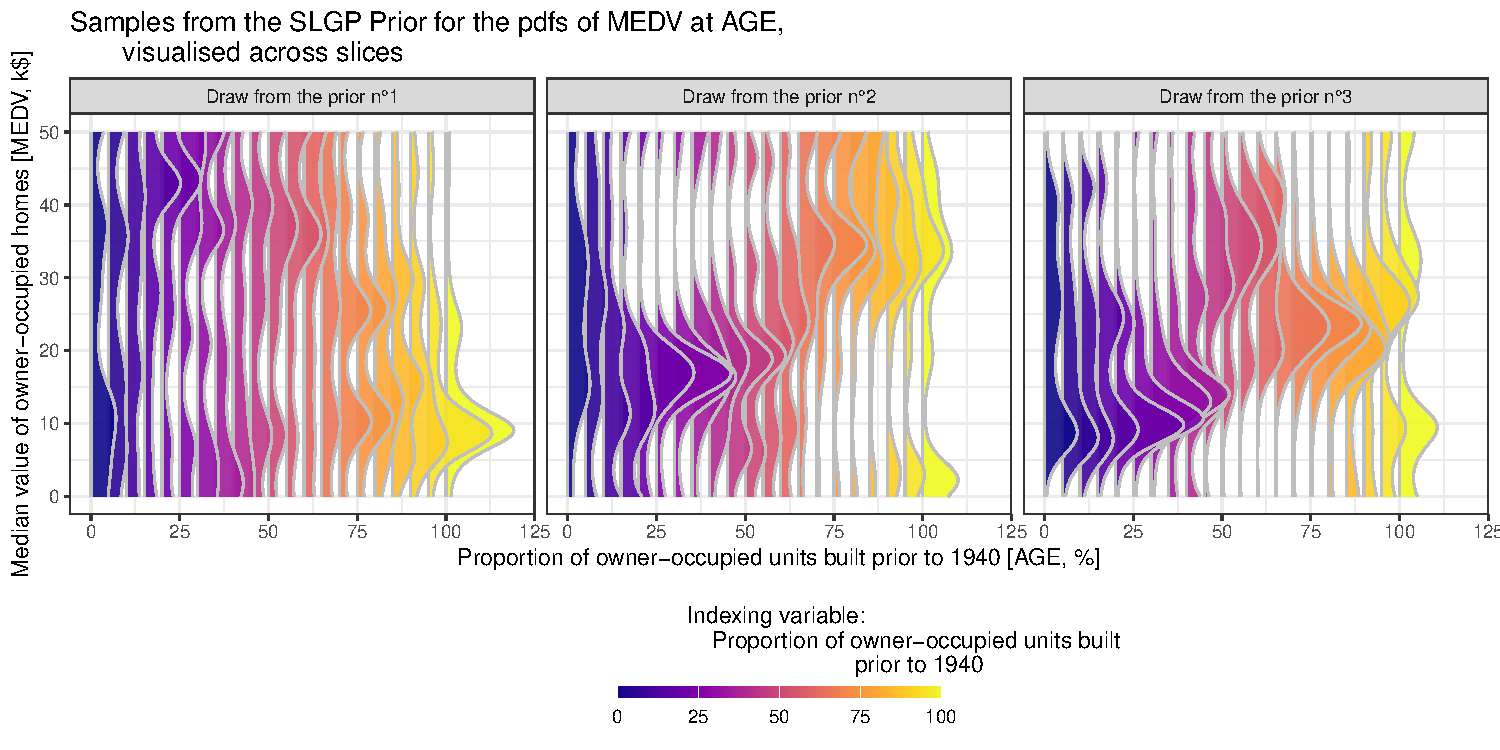
\includegraphics{IntroductionSLGP_files/figure-latex/SLGPplottingPrior1-1} 

}

\caption{Samples from the SLGP Prior for the pdfs of MEDV at AGE, visualised across slices.}\label{fig:SLGPplottingPrior1}
\end{figure}

\begin{Shaded}
\begin{Highlighting}[]
\FunctionTok{ggsave}\NormalTok{(}\FunctionTok{paste0}\NormalTok{(}\StringTok{"./Figures/ribbonsPrior"}\NormalTok{,  }\StringTok{".pdf"}\NormalTok{), }\AttributeTok{width=}\DecValTok{10}\NormalTok{, }\AttributeTok{height=}\DecValTok{5}\NormalTok{)}
\end{Highlighting}
\end{Shaded}

This figure illustrates how the SLGP prior encodes a distribution over densities for different age values. The wide variability indicates the flexibility of SLGPs.

\subsubsection{Assessing whether the flexibility matches that of the data}\label{assessing-whether-the-flexibility-matches-that-of-the-data}

To assess how well the SLGP prior aligns with the actual data distribution, we can also compare it to histograms of \texttt{medv} at selected \texttt{age} values. This visualisation helps us evaluate whether the prior has enough flexibility to represent the observed variability in the data.

\begin{Shaded}
\begin{Highlighting}[]

\NormalTok{selected\_values }\OtherTok{\textless{}{-}} \FunctionTok{c}\NormalTok{(}\DecValTok{20}\NormalTok{, }\DecValTok{50}\NormalTok{, }\DecValTok{95}\NormalTok{)}
\NormalTok{gap }\OtherTok{\textless{}{-}} \DecValTok{5}
\NormalTok{df\_filtered }\OtherTok{\textless{}{-}}\NormalTok{ df }\SpecialCharTok{\%\textgreater{}\%}
  \FunctionTok{mutate}\NormalTok{(}\AttributeTok{interval=}\FunctionTok{findInterval}\NormalTok{(age, }\FunctionTok{c}\NormalTok{(}\DecValTok{0}\NormalTok{, }
\NormalTok{                                      selected\_values[}\DecValTok{1}\NormalTok{]}\SpecialCharTok{{-}}\NormalTok{gap, }
\NormalTok{                                      selected\_values[}\DecValTok{1}\NormalTok{]}\SpecialCharTok{+}\NormalTok{gap, }
\NormalTok{                                      selected\_values[}\DecValTok{2}\NormalTok{]}\SpecialCharTok{{-}}\NormalTok{gap, }
\NormalTok{                                      selected\_values[}\DecValTok{2}\NormalTok{]}\SpecialCharTok{+}\NormalTok{gap, }
\NormalTok{                                      selected\_values[}\DecValTok{3}\NormalTok{]}\SpecialCharTok{{-}}\NormalTok{gap, }
\NormalTok{                                      selected\_values[}\DecValTok{3}\NormalTok{]}\SpecialCharTok{+}\NormalTok{gap)))}\SpecialCharTok{\%\textgreater{}\%}
  \FunctionTok{filter}\NormalTok{(interval }\SpecialCharTok{\%in\%} \FunctionTok{c}\NormalTok{(}\DecValTok{2}\NormalTok{, }\DecValTok{4}\NormalTok{, }\DecValTok{6}\NormalTok{))}\SpecialCharTok{\%\textgreater{}\%}
  \FunctionTok{group\_by}\NormalTok{(interval)}\SpecialCharTok{\%\textgreater{}\%}
  \FunctionTok{mutate}\NormalTok{(}\AttributeTok{category =} \FunctionTok{paste0}\NormalTok{(}\StringTok{"Age close to "}\NormalTok{, }\FunctionTok{c}\NormalTok{(}\StringTok{""}\NormalTok{, selected\_values[}\DecValTok{1}\NormalTok{],}
                                              \StringTok{""}\NormalTok{, selected\_values[}\DecValTok{2}\NormalTok{],}
                                              \StringTok{""}\NormalTok{, selected\_values[}\DecValTok{3}\NormalTok{])[interval], }
                           \StringTok{"}\SpecialCharTok{\textbackslash{}n}\StringTok{n="}\NormalTok{, }\FunctionTok{n}\NormalTok{()))}
\NormalTok{names }\OtherTok{\textless{}{-}} \FunctionTok{sort}\NormalTok{(}\FunctionTok{unique}\NormalTok{(df\_filtered}\SpecialCharTok{$}\NormalTok{category))}
\NormalTok{dfGrid }\OtherTok{\textless{}{-}} \FunctionTok{data.frame}\NormalTok{(}\FunctionTok{expand.grid}\NormalTok{(selected\_values, }
                                 \FunctionTok{seq}\NormalTok{(range\_response[}\DecValTok{1}\NormalTok{], range\_response[}\DecValTok{2}\NormalTok{],, }\DecValTok{101}\NormalTok{)))}
\FunctionTok{colnames}\NormalTok{(dfGrid) }\OtherTok{\textless{}{-}} \FunctionTok{c}\NormalTok{(}\StringTok{"age"}\NormalTok{, }\StringTok{"medv"}\NormalTok{)}
\NormalTok{predPrior }\OtherTok{\textless{}{-}} \FunctionTok{predictSLGP\_newNode}\NormalTok{(}\AttributeTok{SLGPmodel=}\NormalTok{modelPrior,}
                                 \AttributeTok{newNodes =}\NormalTok{ dfGrid)}
\FunctionTok{colnames}\NormalTok{(predPrior) }\OtherTok{\textless{}{-}} \FunctionTok{c}\NormalTok{(}\StringTok{"age"}\NormalTok{, }\StringTok{"medv"}\NormalTok{, }\FunctionTok{paste0}\NormalTok{(}\StringTok{"Draw from the prior n°"}\NormalTok{, }\FunctionTok{seq}\NormalTok{(nrep)))}
\NormalTok{predPrior }\OtherTok{\textless{}{-}}\NormalTok{ predPrior}\SpecialCharTok{\%\textgreater{}\%}
  \FunctionTok{pivot\_longer}\NormalTok{(}\SpecialCharTok{{-}}\FunctionTok{c}\NormalTok{(}\StringTok{"age"}\NormalTok{, }\StringTok{"medv"}\NormalTok{))}
\NormalTok{predPrior}\SpecialCharTok{$}\NormalTok{category }\OtherTok{\textless{}{-}}\FunctionTok{ifelse}\NormalTok{(predPrior}\SpecialCharTok{$}\NormalTok{age}\SpecialCharTok{==}\NormalTok{selected\_values[}\DecValTok{1}\NormalTok{], names[}\DecValTok{1}\NormalTok{],}
                            \FunctionTok{ifelse}\NormalTok{(predPrior}\SpecialCharTok{$}\NormalTok{age}\SpecialCharTok{==}\NormalTok{selected\_values[}\DecValTok{2}\NormalTok{], names[}\DecValTok{2}\NormalTok{], names[}\DecValTok{3}\NormalTok{]))}

\FunctionTok{ggplot}\NormalTok{(}\AttributeTok{mapping=}\FunctionTok{aes}\NormalTok{(}\AttributeTok{x =}\NormalTok{ medv)) }\SpecialCharTok{+}
  \FunctionTok{geom\_histogram}\NormalTok{(df\_filtered,}
                 \AttributeTok{mapping=}\FunctionTok{aes}\NormalTok{(}\AttributeTok{y=}\FunctionTok{after\_stat}\NormalTok{(density)),}
                 \AttributeTok{position =} \StringTok{"identity"}\NormalTok{, }\AttributeTok{breaks =} \FunctionTok{seq}\NormalTok{(}\DecValTok{0}\NormalTok{, }\DecValTok{50}\NormalTok{, }\FloatTok{2.5}\NormalTok{),}
                 \AttributeTok{fill=}\StringTok{"darkgrey"}\NormalTok{, }\AttributeTok{col=}\StringTok{"grey50"}\NormalTok{, }\AttributeTok{lwd=}\FloatTok{0.2}\NormalTok{, }\AttributeTok{alpha=}\FloatTok{0.7}\NormalTok{) }\SpecialCharTok{+}
  \FunctionTok{geom\_rug}\NormalTok{(}\AttributeTok{data=}\NormalTok{df\_filtered, }\AttributeTok{sides =} \StringTok{"b"}\NormalTok{, }\AttributeTok{color =} \StringTok{"navy"}\NormalTok{, }\AttributeTok{alpha =} \FloatTok{0.5}\NormalTok{)}\SpecialCharTok{+}
  \FunctionTok{geom\_line}\NormalTok{(}\AttributeTok{data=}\NormalTok{predPrior, }\AttributeTok{mapping=}\FunctionTok{aes}\NormalTok{(}\AttributeTok{y=}\NormalTok{value, }\AttributeTok{group=}\NormalTok{name), }
            \AttributeTok{color =} \StringTok{"black"}\NormalTok{, }\AttributeTok{lwd=}\FloatTok{0.1}\NormalTok{, }\AttributeTok{alpha=}\FloatTok{0.5}\NormalTok{)}\SpecialCharTok{+}
  \FunctionTok{geom\_line}\NormalTok{(}\AttributeTok{data=}\NormalTok{predPrior, }\AttributeTok{mapping=}\FunctionTok{aes}\NormalTok{(}\AttributeTok{y=}\NormalTok{value, }\AttributeTok{group=}\NormalTok{name, }\AttributeTok{col=}\NormalTok{name), }\AttributeTok{lwd=}\FloatTok{1.1}\NormalTok{)}\SpecialCharTok{+}
  \FunctionTok{facet\_wrap}\NormalTok{(}\SpecialCharTok{\textasciitilde{}}\NormalTok{ category, }\AttributeTok{scales =} \StringTok{"free\_y"}\NormalTok{, }\AttributeTok{nrow=}\DecValTok{1}\NormalTok{) }\SpecialCharTok{+}
  \FunctionTok{labs}\NormalTok{(}\AttributeTok{x =} \StringTok{"Median value of owner{-}occupied homes [k$]"}\NormalTok{, }
       \AttributeTok{y =} \StringTok{"Probability density"}\NormalTok{, }
       \AttributeTok{title =} \StringTok{"Histogram of median value at bins centered at several \textquotesingle{}age\textquotesingle{} values, }
\StringTok{       with width 5}\SpecialCharTok{\textbackslash{}n}\StringTok{versus draws from a SLGP prior"}\NormalTok{) }\SpecialCharTok{+}
  \FunctionTok{theme\_bw}\NormalTok{()}\SpecialCharTok{+}
  \FunctionTok{theme}\NormalTok{(}\AttributeTok{legend.position=}\StringTok{"bottom"}\NormalTok{,}
        \AttributeTok{legend.direction =} \StringTok{"horizontal"}\NormalTok{,}
        \AttributeTok{legend.title =} \FunctionTok{element\_blank}\NormalTok{())}\SpecialCharTok{+}
  \FunctionTok{coord\_cartesian}\NormalTok{(}\AttributeTok{xlim=}\NormalTok{range\_response,}
                  \AttributeTok{ylim=}\FunctionTok{c}\NormalTok{(}\DecValTok{0}\NormalTok{, }\FloatTok{0.25}\NormalTok{))}
\end{Highlighting}
\end{Shaded}

\begin{figure}[H]

{\centering 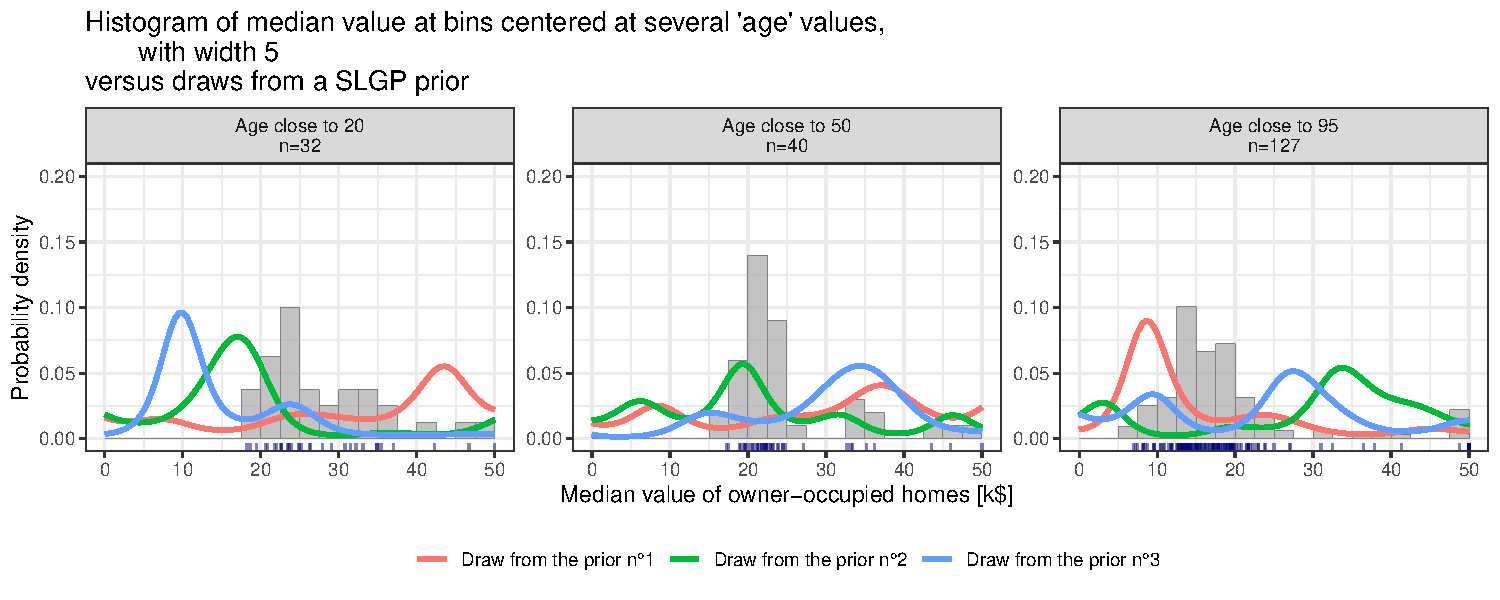
\includegraphics{IntroductionSLGP_files/figure-latex/SLGPplottingPrior2-1} 

}

\caption{Samples from the SLGP Prior versus histograms of median value at bins centered at several 'age' values}\label{fig:SLGPplottingPrior2}
\end{figure}

\begin{Shaded}
\begin{Highlighting}[]

\FunctionTok{ggsave}\NormalTok{(}\FunctionTok{paste0}\NormalTok{(}\StringTok{"./Figures/histPrior"}\NormalTok{,  }\StringTok{".pdf"}\NormalTok{), }\AttributeTok{width=}\DecValTok{10}\NormalTok{, }\AttributeTok{height=}\DecValTok{5}\NormalTok{)}
\end{Highlighting}
\end{Shaded}

Since this is a prior distribution, it does not yet incorporate information from the actual data. Therefore, we should not expect it to match the empirical histograms. However, the prior samples display a reasonable level of variability and structure, suggesting that the model would be well-suited for density estimation after incorporating data through posterior inference.

\subsubsection{Other priors}\label{other-priors}

To explore how different covariance structures influence the SLGP prior, we compare three additional kernel choices:

\begin{itemize}
\tightlist
\item
  Exponential Kernel: A special case of the Matérn class (\(\nu\) = 1/2) that results in less smooth realizations.
\item
  Matérn 3/2 Kernel: A compromise between flexibility and smoothness.
\item
  Gaussian Kernel: The limiting case, leading to infinitely differentiable functions.
\end{itemize}

\begin{Shaded}
\begin{Highlighting}[]
\CommentTok{\# With exponential kernel}
\NormalTok{modelPrior2 }\OtherTok{\textless{}{-}} \FunctionTok{slgp}\NormalTok{(medv}\SpecialCharTok{\textasciitilde{}}\NormalTok{age, }
                    \AttributeTok{data=}\NormalTok{df,}
                    \AttributeTok{method=}\StringTok{"none"}\NormalTok{, }
                    \AttributeTok{basisFunctionsUsed =} \StringTok{"RFF"}\NormalTok{,}
                    \AttributeTok{interpolateBasisFun=}\StringTok{"WNN"}\NormalTok{, }
                    \AttributeTok{hyperparams =} \FunctionTok{list}\NormalTok{(}\AttributeTok{lengthscale=}\FunctionTok{c}\NormalTok{(}\FloatTok{0.15}\NormalTok{, }\FloatTok{0.15}\NormalTok{), }
                                       \AttributeTok{sigma2=}\DecValTok{1}\NormalTok{), }
                    \AttributeTok{sigmaEstimationMethod =} \StringTok{"heuristic"}\NormalTok{, }
                    \AttributeTok{predictorsLower=} \FunctionTok{c}\NormalTok{(range\_x[}\DecValTok{1}\NormalTok{]),}
                    \AttributeTok{predictorsUpper=} \FunctionTok{c}\NormalTok{(range\_x[}\DecValTok{2}\NormalTok{]),}
                    \AttributeTok{responseRange=}\NormalTok{ range\_response,}
                    \AttributeTok{opts\_BasisFun =} \FunctionTok{list}\NormalTok{(}\AttributeTok{nFreq=}\DecValTok{200}\NormalTok{,}
                                         \AttributeTok{MatParam=}\DecValTok{1}\SpecialCharTok{/}\DecValTok{2}\NormalTok{),}
                    \AttributeTok{seed=}\DecValTok{1}\NormalTok{)}
\CommentTok{\# With Matérn 3/2 kernel}
\NormalTok{modelPrior3 }\OtherTok{\textless{}{-}} \FunctionTok{slgp}\NormalTok{(medv}\SpecialCharTok{\textasciitilde{}}\NormalTok{age, }
                    \AttributeTok{data=}\NormalTok{df,}
                    \AttributeTok{method=}\StringTok{"none"}\NormalTok{, }
                    \AttributeTok{basisFunctionsUsed =} \StringTok{"RFF"}\NormalTok{,}
                    \AttributeTok{interpolateBasisFun=}\StringTok{"WNN"}\NormalTok{, }
                    \AttributeTok{hyperparams =} \FunctionTok{list}\NormalTok{(}\AttributeTok{lengthscale=}\FunctionTok{c}\NormalTok{(}\FloatTok{0.15}\NormalTok{, }\FloatTok{0.15}\NormalTok{), }
                                       \AttributeTok{sigma2=}\DecValTok{1}\NormalTok{), }
                    \AttributeTok{sigmaEstimationMethod =} \StringTok{"heuristic"}\NormalTok{, }
                    \AttributeTok{predictorsLower=} \FunctionTok{c}\NormalTok{(range\_x[}\DecValTok{1}\NormalTok{]),}
                    \AttributeTok{predictorsUpper=} \FunctionTok{c}\NormalTok{(range\_x[}\DecValTok{2}\NormalTok{]),}
                    \AttributeTok{responseRange=}\NormalTok{ range\_response,}
                    \AttributeTok{opts\_BasisFun =} \FunctionTok{list}\NormalTok{(}\AttributeTok{nFreq=}\DecValTok{200}\NormalTok{,}
                                         \AttributeTok{MatParam=}\DecValTok{3}\SpecialCharTok{/}\DecValTok{2}\NormalTok{),}
                    \AttributeTok{seed=}\DecValTok{1}\NormalTok{)}
\CommentTok{\# with Gaussian Kernel}
\NormalTok{modelPrior4 }\OtherTok{\textless{}{-}} \FunctionTok{slgp}\NormalTok{(medv}\SpecialCharTok{\textasciitilde{}}\NormalTok{age, }
                    \AttributeTok{data=}\NormalTok{df,}
                    \AttributeTok{method=}\StringTok{"none"}\NormalTok{, }
                    \AttributeTok{basisFunctionsUsed =} \StringTok{"RFF"}\NormalTok{,}
                    \AttributeTok{interpolateBasisFun=}\StringTok{"WNN"}\NormalTok{, }
                    \AttributeTok{hyperparams =} \FunctionTok{list}\NormalTok{(}\AttributeTok{lengthscale=}\FunctionTok{c}\NormalTok{(}\FloatTok{0.15}\NormalTok{, }\FloatTok{0.15}\NormalTok{), }
                                       \AttributeTok{sigma2=}\DecValTok{1}\NormalTok{), }
                    \AttributeTok{sigmaEstimationMethod =} \StringTok{"heuristic"}\NormalTok{, }
                    \AttributeTok{predictorsLower=} \FunctionTok{c}\NormalTok{(range\_x[}\DecValTok{1}\NormalTok{]),}
                    \AttributeTok{predictorsUpper=} \FunctionTok{c}\NormalTok{(range\_x[}\DecValTok{2}\NormalTok{]),}
                    \AttributeTok{responseRange=}\NormalTok{ range\_response,}
                    \AttributeTok{opts\_BasisFun =} \FunctionTok{list}\NormalTok{(}\AttributeTok{nFreq=}\DecValTok{200}\NormalTok{,}
                                         \AttributeTok{MatParam=}\ConstantTok{Inf}\NormalTok{),}
                    \AttributeTok{seed=}\DecValTok{1}\NormalTok{)}
\end{Highlighting}
\end{Shaded}

The figure below visualizes samples from the priors corresponding to each kernel. While the overall behavior remains similar, the choice of kernel influences the smoothness of the density estimates. The exponential kernel exhibits the most variability, while the Gaussian kernel enforces stronger smoothness constraints.

\begin{Shaded}
\begin{Highlighting}[]
\NormalTok{nrep }\OtherTok{\textless{}{-}} \DecValTok{1}
\FunctionTok{set.seed}\NormalTok{(}\DecValTok{1}\NormalTok{)}
\NormalTok{coef }\OtherTok{\textless{}{-}} \FunctionTok{matrix}\NormalTok{(}\FunctionTok{rnorm}\NormalTok{(}\AttributeTok{n=}\NormalTok{nrep}\SpecialCharTok{*}\NormalTok{p), }\AttributeTok{nrow=}\NormalTok{nrep)}
\NormalTok{modelPrior2}\SpecialCharTok{@}\NormalTok{coefficients }\OtherTok{\textless{}{-}}\NormalTok{ coef}
\NormalTok{modelPrior3}\SpecialCharTok{@}\NormalTok{coefficients }\OtherTok{\textless{}{-}}\NormalTok{ coef}
\NormalTok{modelPrior4}\SpecialCharTok{@}\NormalTok{coefficients }\OtherTok{\textless{}{-}}\NormalTok{ coef}

\NormalTok{dfGrid }\OtherTok{\textless{}{-}} \FunctionTok{data.frame}\NormalTok{(}\FunctionTok{expand.grid}\NormalTok{(}\FunctionTok{seq}\NormalTok{(range\_x[}\DecValTok{1}\NormalTok{], range\_x[}\DecValTok{2}\NormalTok{], }\DecValTok{5}\NormalTok{), }
                                 \FunctionTok{seq}\NormalTok{(range\_response[}\DecValTok{1}\NormalTok{], range\_response[}\DecValTok{2}\NormalTok{],, }\DecValTok{101}\NormalTok{)))}
\FunctionTok{colnames}\NormalTok{(dfGrid) }\OtherTok{\textless{}{-}} \FunctionTok{c}\NormalTok{(}\StringTok{"age"}\NormalTok{, }\StringTok{"medv"}\NormalTok{)}

\NormalTok{predPrior }\OtherTok{\textless{}{-}} \FunctionTok{rbind}\NormalTok{(}\FunctionTok{predictSLGP\_newNode}\NormalTok{(}\AttributeTok{SLGPmodel=}\NormalTok{modelPrior2,}
                                       \AttributeTok{newNodes =}\NormalTok{ dfGrid),}
                   \FunctionTok{predictSLGP\_newNode}\NormalTok{(}\AttributeTok{SLGPmodel=}\NormalTok{modelPrior3,}
                                       \AttributeTok{newNodes =}\NormalTok{ dfGrid),}
                   \FunctionTok{predictSLGP\_newNode}\NormalTok{(}\AttributeTok{SLGPmodel=}\NormalTok{modelPrior4,}
                                       \AttributeTok{newNodes =}\NormalTok{ dfGrid))}
\NormalTok{predPrior}\SpecialCharTok{$}\NormalTok{Kernel }\OtherTok{\textless{}{-}} \FunctionTok{c}\NormalTok{(}\FunctionTok{sapply}\NormalTok{(}\FunctionTok{seq}\NormalTok{(}\DecValTok{3}\NormalTok{), }\ControlFlowTok{function}\NormalTok{(i)\{}\FunctionTok{rep}\NormalTok{(i, }\FunctionTok{nrow}\NormalTok{(dfGrid))\}))}
\FunctionTok{colnames}\NormalTok{(predPrior) }\OtherTok{\textless{}{-}} \FunctionTok{c}\NormalTok{(}\StringTok{"age"}\NormalTok{, }\StringTok{"medv"}\NormalTok{, }\StringTok{"value"}\NormalTok{, }\StringTok{"Kernel"}\NormalTok{)}

\NormalTok{predPrior}\SpecialCharTok{$}\NormalTok{Kernel }\OtherTok{\textless{}{-}} \FunctionTok{factor}\NormalTok{(}\FunctionTok{c}\NormalTok{(}\StringTok{"Exponential"}\NormalTok{, }\StringTok{"Matérn 3/2"}\NormalTok{, }\StringTok{"Gaussian"}\NormalTok{)[predPrior}\SpecialCharTok{$}\NormalTok{Kernel], }
                           \AttributeTok{levels=}\FunctionTok{c}\NormalTok{(}\StringTok{"Exponential"}\NormalTok{, }\StringTok{"Matérn 3/2"}\NormalTok{, }\StringTok{"Gaussian"}\NormalTok{))}
\NormalTok{scale\_factor }\OtherTok{\textless{}{-}} \DecValTok{200}
\FunctionTok{ggplot}\NormalTok{()  }\SpecialCharTok{+}
  \FunctionTok{labs}\NormalTok{(}\AttributeTok{y =} \StringTok{"Proportion of owner{-}occupied units built prior to 1940 [AGE, \%]"}\NormalTok{, }
       \AttributeTok{x =} \StringTok{"Median value of owner{-}occupied homes [MEDV, k$]"}\NormalTok{,}
       \AttributeTok{title =} \StringTok{"Samples from SLGP Priors with varying smoothnesses for the pdfs of MEDV at AGE, visualised across slices"}\NormalTok{) }\SpecialCharTok{+}
  \FunctionTok{theme\_bw}\NormalTok{()}\SpecialCharTok{+}
  \FunctionTok{geom\_ribbon}\NormalTok{(}\AttributeTok{data=}\NormalTok{predPrior,}
              \AttributeTok{mapping=}\FunctionTok{aes}\NormalTok{(}\AttributeTok{x=}\NormalTok{medv, }\AttributeTok{ymax=}\NormalTok{scale\_factor}\SpecialCharTok{*}\NormalTok{value}\SpecialCharTok{+}\NormalTok{age, }
                          \AttributeTok{ymin=}\NormalTok{age, }\AttributeTok{group=}\SpecialCharTok{{-}}\NormalTok{age, }\AttributeTok{fill=}\NormalTok{age),}
              \AttributeTok{col=}\StringTok{"grey"}\NormalTok{, }\AttributeTok{alpha=}\FloatTok{0.9}\NormalTok{)}\SpecialCharTok{+}
  \FunctionTok{scale\_fill\_viridis}\NormalTok{(}\AttributeTok{option =} \StringTok{"plasma"}\NormalTok{,}
                     \AttributeTok{guide =} \FunctionTok{guide\_colorbar}\NormalTok{(}\AttributeTok{nrow =} \DecValTok{1}\NormalTok{,}
                                            \AttributeTok{title =} \StringTok{"Indexing variable: }
\StringTok{                                            Proportion of owner{-}occupied units built }
\StringTok{                                            prior to 1940"}\NormalTok{,}
                                            \AttributeTok{barheight =} \FunctionTok{unit}\NormalTok{(}\DecValTok{2}\NormalTok{, }\AttributeTok{units =} \StringTok{"mm"}\NormalTok{),}
                                            \AttributeTok{barwidth =} \FunctionTok{unit}\NormalTok{(}\DecValTok{55}\NormalTok{, }\AttributeTok{units =} \StringTok{"mm"}\NormalTok{),}
                                            \AttributeTok{title.position =} \StringTok{\textquotesingle{}top\textquotesingle{}}\NormalTok{,}
                                            \AttributeTok{label.position =} \StringTok{"bottom"}\NormalTok{,}
                                            \AttributeTok{title.hjust =} \FloatTok{0.5}\NormalTok{))}\SpecialCharTok{+}
  \FunctionTok{theme}\NormalTok{(}\AttributeTok{legend.position =} \StringTok{"bottom"}\NormalTok{)}\SpecialCharTok{+}
  \FunctionTok{coord\_flip}\NormalTok{()}\SpecialCharTok{+}
  \FunctionTok{facet\_grid}\NormalTok{(.}\SpecialCharTok{\textasciitilde{}}\NormalTok{Kernel)}
\end{Highlighting}
\end{Shaded}

\begin{figure}[H]

{\centering 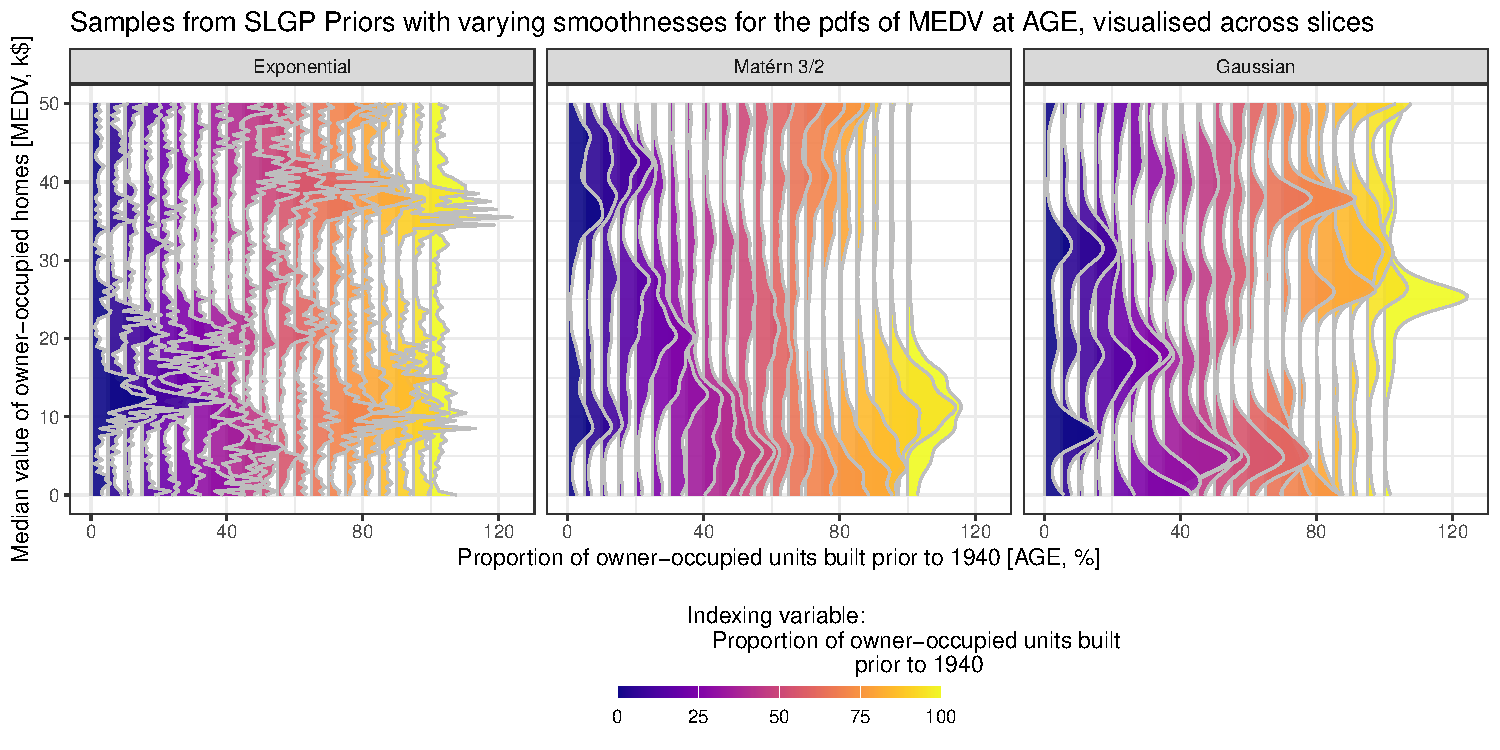
\includegraphics{IntroductionSLGP_files/figure-latex/SLGPplottingOtherPrior1-1} 

}

\caption{Samples from the other SLGP Priors for the pdfs of MEDV at AGE, visualised across slices.}\label{fig:SLGPplottingOtherPrior1}
\end{figure}

\begin{Shaded}
\begin{Highlighting}[]
\FunctionTok{ggsave}\NormalTok{(}\FunctionTok{paste0}\NormalTok{(}\StringTok{"./Figures/ribbonsPriorOthers"}\NormalTok{,  }\StringTok{".pdf"}\NormalTok{), }\AttributeTok{width=}\DecValTok{10}\NormalTok{, }\AttributeTok{height=}\DecValTok{5}\NormalTok{)}
\end{Highlighting}
\end{Shaded}

\subsection{Estimation: Maximum a posteriori estimate}\label{estimation-maximum-a-posteriori-estimate}

For a fast and computationally efficient estimation, we propose using MAP estimation. MAP delivers a single point estimate by maximizing the posterior distribution. It is the fastest estimation scheme we propose, however MAP does not facilitate uncertainty quantification because it yields a non-probabilistic estimate of the underlying density field, focusing instead on identifying the mode of the posterior distribution.

\subsubsection{Performing the estimation}\label{performing-the-estimation}

We demonstrate three equivalent ways to train an SLGP model using our package:

\begin{itemize}
\item
  Direct initialization: Computes the basis functions and performs the full estimation from scratch.
\item
  Retraining from another model: Reuses pre-computed basis functions from an existing SLGP model and updates only the coefficients for efficiency.
\item
  Explicit reuse of prior components: Allows manually specifying pre-computed basis functions, offering greater control over the initialization.
\end{itemize}

\begin{Shaded}
\begin{Highlighting}[]
\NormalTok{modelMAP }\OtherTok{\textless{}{-}} \FunctionTok{slgp}\NormalTok{(medv}\SpecialCharTok{\textasciitilde{}}\NormalTok{age, }\CommentTok{\# Use a formula to specify predictors VS response}
                 \CommentTok{\# Can use medv\textasciitilde{}. for all variables,}
                 \CommentTok{\# Or medv \textasciitilde{} age + var2 + var3 for more variables}
                 \AttributeTok{data=}\NormalTok{df,}
                 \AttributeTok{method=}\StringTok{"MAP"}\NormalTok{, }\CommentTok{\#Maximum a posteriori estimation scheme}
                 \AttributeTok{basisFunctionsUsed =} \StringTok{"RFF"}\NormalTok{,}
                 \AttributeTok{interpolateBasisFun=}\StringTok{"WNN"}\NormalTok{, }\CommentTok{\# Accelerate inference}
                 \AttributeTok{hyperparams =} \FunctionTok{list}\NormalTok{(}\AttributeTok{lengthscale=}\FunctionTok{c}\NormalTok{(}\FloatTok{0.15}\NormalTok{, }\FloatTok{0.15}\NormalTok{), }
                                    \CommentTok{\# Applied to normalised data}
                                    \CommentTok{\# So 0.15 is 15\% of the range of values}
                                    \AttributeTok{sigma2=}\DecValTok{1}\NormalTok{), }
                 \CommentTok{\# Will be re{-}selected with sigmaEstimationMethod}
                 \AttributeTok{sigmaEstimationMethod =} \StringTok{"heuristic"}\NormalTok{, }
                 \CommentTok{\# Set to heuristic for numerical stability                 }
                 \AttributeTok{predictorsLower=} \FunctionTok{c}\NormalTok{(range\_x[}\DecValTok{1}\NormalTok{]),}
                 \AttributeTok{predictorsUpper=} \FunctionTok{c}\NormalTok{(range\_x[}\DecValTok{2}\NormalTok{]),}
                 \AttributeTok{responseRange=}\NormalTok{ range\_response,}
                 \AttributeTok{opts\_BasisFun =} \FunctionTok{list}\NormalTok{(}\AttributeTok{nFreq=}\DecValTok{200}\NormalTok{,}
                                      \AttributeTok{MatParam=}\DecValTok{5}\SpecialCharTok{/}\DecValTok{2}\NormalTok{),}
                 \AttributeTok{seed=}\DecValTok{1}\NormalTok{)}
\end{Highlighting}
\end{Shaded}

\begin{Shaded}
\begin{Highlighting}[]
\CommentTok{\# Or equivalent, re{-}use the same basis functions }
\CommentTok{\# and hyper parameters as in the prior we saw}

\NormalTok{modelMAP }\OtherTok{\textless{}{-}} \FunctionTok{retrainSLGP}\NormalTok{(}\AttributeTok{SLGPmodel=}\NormalTok{modelPrior, }
                        \AttributeTok{newdata =}\NormalTok{ df, }
                        \AttributeTok{method=}\StringTok{"MAP"}\NormalTok{)}
\end{Highlighting}
\end{Shaded}

\begin{Shaded}
\begin{Highlighting}[]
\CommentTok{\# Or equivalent, more explicit in the re{-}using of the elements}
\CommentTok{\# From the SLGP prior}

\NormalTok{modelMAP }\OtherTok{\textless{}{-}} \FunctionTok{slgp}\NormalTok{(medv}\SpecialCharTok{\textasciitilde{}}\NormalTok{age, }
                 \AttributeTok{data=}\NormalTok{df,}
                 \AttributeTok{method=}\StringTok{"MAP"}\NormalTok{, }\CommentTok{\#Maximum a posteriori estimation scheme}
                 \AttributeTok{basisFunctionsUsed =} \StringTok{"RFF"}\NormalTok{,}
                 \AttributeTok{interpolateBasisFun=}\StringTok{"WNN"}\NormalTok{, }\CommentTok{\# Accelerate inference}
                 \AttributeTok{hyperparams =}\NormalTok{ modelPrior}\SpecialCharTok{@}\NormalTok{hyperparams, }
                 \AttributeTok{sigmaEstimationMethod =} \StringTok{"none"}\NormalTok{,}\CommentTok{\# Already selected in the prior}
                 \AttributeTok{predictorsLower=} \FunctionTok{c}\NormalTok{(range\_x[}\DecValTok{1}\NormalTok{]),}
                 \AttributeTok{predictorsUpper=} \FunctionTok{c}\NormalTok{(range\_x[}\DecValTok{2}\NormalTok{]),}
                 \AttributeTok{responseRange=}\NormalTok{ range\_response,}
                 \AttributeTok{opts\_BasisFun =}\NormalTok{ modelPrior}\SpecialCharTok{@}\NormalTok{opts\_BasisFun,}
                 \AttributeTok{BasisFunParam =}\NormalTok{ modelPrior}\SpecialCharTok{@}\NormalTok{BasisFunParam,}
                 \AttributeTok{seed=}\DecValTok{1}\NormalTok{)}
\end{Highlighting}
\end{Shaded}

\subsubsection{Visualising the results}\label{visualising-the-results}

The estimated conditional density function is displayed using two different representations:

\begin{itemize}
\item
  A colormap showing the predicted density of medv as a function of age.
\item
  A ribbon plot, which slices the conditional density at selected age values to provide a clearer view of the estimated distributions.
\end{itemize}

\begin{Shaded}
\begin{Highlighting}[]
\NormalTok{dfGrid }\OtherTok{\textless{}{-}} \FunctionTok{data.frame}\NormalTok{(}\FunctionTok{expand.grid}\NormalTok{(}\FunctionTok{seq}\NormalTok{(range\_x[}\DecValTok{1}\NormalTok{], range\_x[}\DecValTok{2}\NormalTok{],, }\DecValTok{101}\NormalTok{), }
                                 \FunctionTok{seq}\NormalTok{(range\_response[}\DecValTok{1}\NormalTok{], range\_response[}\DecValTok{2}\NormalTok{],, }\DecValTok{101}\NormalTok{)))}
\FunctionTok{colnames}\NormalTok{(dfGrid) }\OtherTok{\textless{}{-}} \FunctionTok{c}\NormalTok{(}\StringTok{"age"}\NormalTok{, }\StringTok{"medv"}\NormalTok{)}
\NormalTok{pred }\OtherTok{\textless{}{-}} \FunctionTok{predictSLGP\_newNode}\NormalTok{(}\AttributeTok{SLGPmodel=}\NormalTok{modelMAP,}
                            \AttributeTok{newNodes =}\NormalTok{ dfGrid)}

\FunctionTok{ggplot}\NormalTok{()  }\SpecialCharTok{+}
  \FunctionTok{labs}\NormalTok{(}\AttributeTok{y =} \StringTok{"Proportion of owner{-}occupied units}\SpecialCharTok{\textbackslash{}n}\StringTok{built prior to 1940 [\%]"}\NormalTok{, }
       \AttributeTok{x =} \StringTok{"Median value of owner{-}occupied homes [k$]"}\NormalTok{,}
       \AttributeTok{title =} \StringTok{"Median value vs. age of homes"}\NormalTok{) }\SpecialCharTok{+}
  \FunctionTok{theme\_bw}\NormalTok{()}\SpecialCharTok{+}
  \FunctionTok{geom\_raster}\NormalTok{(}\AttributeTok{data=}\NormalTok{pred,}
              \AttributeTok{mapping=}\FunctionTok{aes}\NormalTok{(}\AttributeTok{x=}\NormalTok{age, }\AttributeTok{y=}\NormalTok{medv, }\AttributeTok{fill=}\NormalTok{pdf\_1))}\SpecialCharTok{+}
  \FunctionTok{geom\_point}\NormalTok{(}\AttributeTok{data=}\NormalTok{df,}
             \AttributeTok{mapping=}\FunctionTok{aes}\NormalTok{(}\AttributeTok{x=}\NormalTok{age, }\AttributeTok{y=}\NormalTok{medv), }\AttributeTok{alpha =} \FloatTok{0.5}\NormalTok{, }
             \AttributeTok{pch=}\StringTok{"x"}\NormalTok{, }\AttributeTok{col=}\StringTok{"grey"}\NormalTok{)}\SpecialCharTok{+}
  \FunctionTok{scale\_fill\_viridis}\NormalTok{(}\AttributeTok{option =} \StringTok{"viridis"}\NormalTok{,}
                     \AttributeTok{guide =} \FunctionTok{guide\_colorbar}\NormalTok{(}\AttributeTok{nrow =} \DecValTok{1}\NormalTok{,}
                                            \AttributeTok{title =} \StringTok{"Probability density of med at age"}\NormalTok{,}
                                            \AttributeTok{barheight =} \FunctionTok{unit}\NormalTok{(}\DecValTok{2}\NormalTok{, }\AttributeTok{units =} \StringTok{"mm"}\NormalTok{),}
                                            \AttributeTok{barwidth =} \FunctionTok{unit}\NormalTok{(}\DecValTok{55}\NormalTok{, }\AttributeTok{units =} \StringTok{"mm"}\NormalTok{),}
                                            \AttributeTok{title.position =} \StringTok{\textquotesingle{}top\textquotesingle{}}\NormalTok{,}
                                            \AttributeTok{label.position =} \StringTok{"bottom"}\NormalTok{,}
                                            \AttributeTok{title.hjust =} \FloatTok{0.5}\NormalTok{))}\SpecialCharTok{+}
  \FunctionTok{theme}\NormalTok{(}\AttributeTok{legend.position =} \StringTok{"bottom"}\NormalTok{)}
\end{Highlighting}
\end{Shaded}

\begin{figure}[H]

{\centering 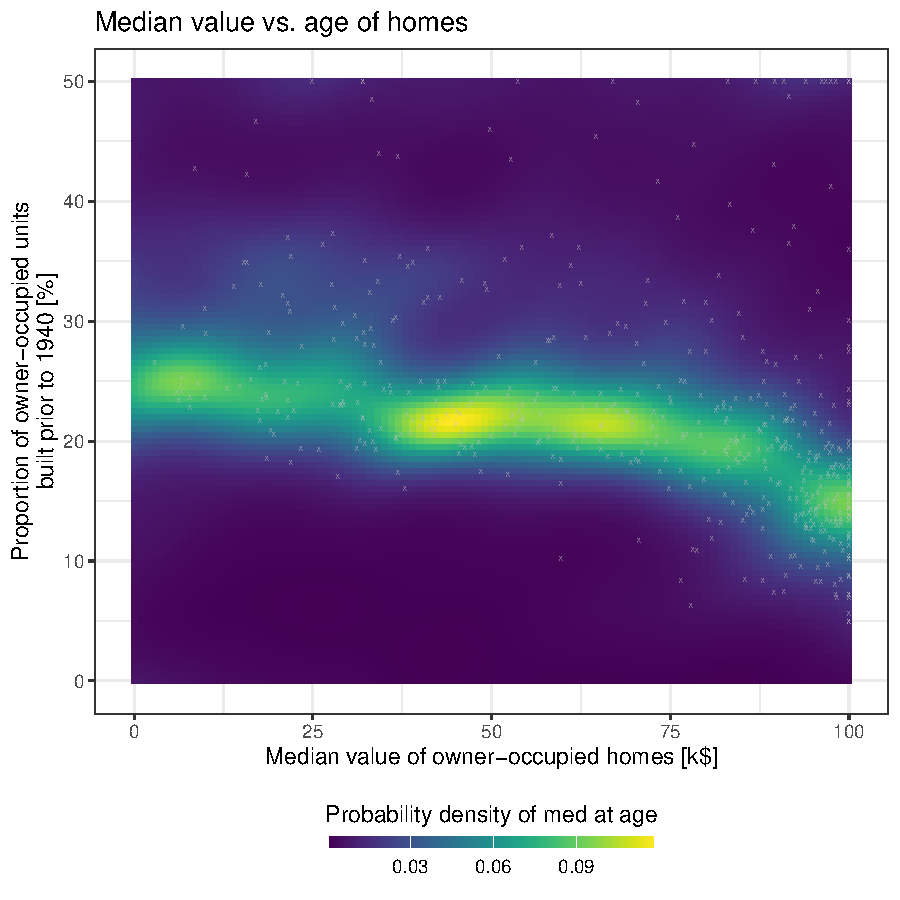
\includegraphics{IntroductionSLGP_files/figure-latex/SLGPplotting1-1} 

}

\caption{Predictive probability density of medv at age, as predicted by a SLGP.}\label{fig:SLGPplotting1}
\end{figure}

\begin{Shaded}
\begin{Highlighting}[]

\FunctionTok{library}\NormalTok{(viridis)}
\NormalTok{dfGrid }\OtherTok{\textless{}{-}} \FunctionTok{data.frame}\NormalTok{(}\FunctionTok{expand.grid}\NormalTok{(}\FunctionTok{seq}\NormalTok{(range\_x[}\DecValTok{1}\NormalTok{], range\_x[}\DecValTok{2}\NormalTok{], }\DecValTok{5}\NormalTok{), }
                                 \FunctionTok{seq}\NormalTok{(range\_response[}\DecValTok{1}\NormalTok{], range\_response[}\DecValTok{2}\NormalTok{],, }\DecValTok{101}\NormalTok{)))}
\FunctionTok{colnames}\NormalTok{(dfGrid) }\OtherTok{\textless{}{-}} \FunctionTok{c}\NormalTok{(}\StringTok{"age"}\NormalTok{, }\StringTok{"medv"}\NormalTok{)}
\NormalTok{pred }\OtherTok{\textless{}{-}} \FunctionTok{predictSLGP\_newNode}\NormalTok{(}\AttributeTok{SLGPmodel=}\NormalTok{modelMAP,}
                            \AttributeTok{newNodes =}\NormalTok{ dfGrid)}

\NormalTok{scale\_factor }\OtherTok{\textless{}{-}} \DecValTok{100}
\FunctionTok{ggplot}\NormalTok{()  }\SpecialCharTok{+}
  \FunctionTok{labs}\NormalTok{(}\AttributeTok{y =} \StringTok{"Proportion of owner{-}occupied units}\SpecialCharTok{\textbackslash{}n}\StringTok{built prior to 1940 [\%]"}\NormalTok{, }
       \AttributeTok{x =} \StringTok{"Median value of owner{-}occupied homes [k$]"}\NormalTok{,}
       \AttributeTok{title =} \StringTok{"Median value vs. age of homes"}\NormalTok{) }\SpecialCharTok{+}
  \FunctionTok{theme\_bw}\NormalTok{()}\SpecialCharTok{+}
  \FunctionTok{geom\_ribbon}\NormalTok{(}\AttributeTok{data=}\NormalTok{pred,}
              \AttributeTok{mapping=}\FunctionTok{aes}\NormalTok{(}\AttributeTok{x=}\NormalTok{medv, }\AttributeTok{ymax=}\NormalTok{scale\_factor}\SpecialCharTok{*}\NormalTok{pdf\_1}\SpecialCharTok{+}\NormalTok{age, }
                          \AttributeTok{ymin=}\NormalTok{age, }\AttributeTok{group=}\SpecialCharTok{{-}}\NormalTok{age, }\AttributeTok{fill=}\NormalTok{age),}
              \AttributeTok{col=}\StringTok{"grey"}\NormalTok{, }\AttributeTok{alpha=}\FloatTok{0.9}\NormalTok{)}\SpecialCharTok{+}
  \FunctionTok{geom\_point}\NormalTok{(}\AttributeTok{data=}\NormalTok{df,}
             \AttributeTok{mapping=}\FunctionTok{aes}\NormalTok{(}\AttributeTok{x =}\NormalTok{ medv, }\AttributeTok{y =}\NormalTok{ age), }\AttributeTok{alpha =} \FloatTok{0.5}\NormalTok{, }\AttributeTok{color =} \StringTok{"navy"}\NormalTok{)}\SpecialCharTok{+}
  \FunctionTok{scale\_fill\_viridis}\NormalTok{(}\AttributeTok{option =} \StringTok{"plasma"}\NormalTok{,}
                     \AttributeTok{guide =} \FunctionTok{guide\_colorbar}\NormalTok{(}\AttributeTok{nrow =} \DecValTok{1}\NormalTok{,}
                                            \AttributeTok{title =} \StringTok{"Indexing variable: }
\StringTok{                                            Proportion of owner{-}occupied units built }
\StringTok{                                            prior to 1940"}\NormalTok{,}
                                            \AttributeTok{barheight =} \FunctionTok{unit}\NormalTok{(}\DecValTok{2}\NormalTok{, }\AttributeTok{units =} \StringTok{"mm"}\NormalTok{),}
                                            \AttributeTok{barwidth =} \FunctionTok{unit}\NormalTok{(}\DecValTok{55}\NormalTok{, }\AttributeTok{units =} \StringTok{"mm"}\NormalTok{),}
                                            \AttributeTok{title.position =} \StringTok{\textquotesingle{}top\textquotesingle{}}\NormalTok{,}
                                            \AttributeTok{label.position =} \StringTok{"bottom"}\NormalTok{,}
                                            \AttributeTok{title.hjust =} \FloatTok{0.5}\NormalTok{))}\SpecialCharTok{+}
  \FunctionTok{theme}\NormalTok{(}\AttributeTok{legend.position =} \StringTok{"bottom"}\NormalTok{)}\SpecialCharTok{+}
  \FunctionTok{coord\_flip}\NormalTok{()}
\end{Highlighting}
\end{Shaded}

\begin{figure}[H]

{\centering 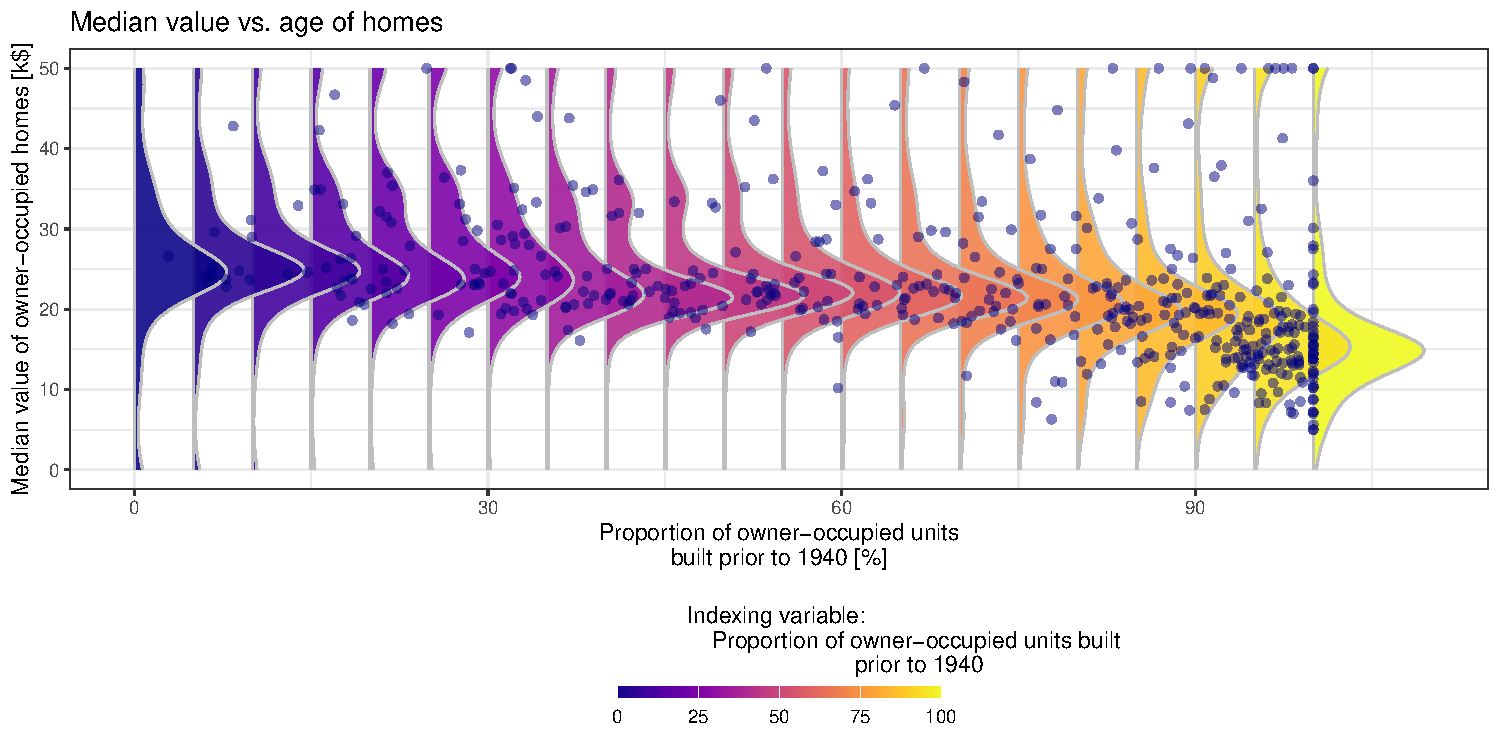
\includegraphics{IntroductionSLGP_files/figure-latex/SLGPplotting2-1} 

}

\caption{Predictive probability density of medv at age, seen over slices.}\label{fig:SLGPplotting2}
\end{figure}

\begin{Shaded}
\begin{Highlighting}[]
\FunctionTok{ggsave}\NormalTok{(}\FunctionTok{paste0}\NormalTok{(}\StringTok{"./Figures/ribbonsMAP"}\NormalTok{,  }\StringTok{".pdf"}\NormalTok{), }\AttributeTok{width=}\DecValTok{10}\NormalTok{, }\AttributeTok{height=}\DecValTok{5}\NormalTok{)}
\end{Highlighting}
\end{Shaded}

The figure reveals how the SLGP captures the structure in the estimated conditional density of \texttt{medv} given \texttt{age}. It effectively adapts to variations in skewness as the distribution of home prices shifts across different property ages. Notably, the model also captures the survivor bias we noted earlier by assigning a small but notable probability mass to older units with high values.

\subsubsection{Comparing the estimation to data}\label{comparing-the-estimation-to-data}

\begin{Shaded}
\begin{Highlighting}[]

\NormalTok{selected\_values }\OtherTok{\textless{}{-}} \FunctionTok{c}\NormalTok{(}\DecValTok{20}\NormalTok{, }\DecValTok{50}\NormalTok{, }\DecValTok{95}\NormalTok{)}
\NormalTok{gap }\OtherTok{\textless{}{-}} \DecValTok{5}
\NormalTok{df\_filtered }\OtherTok{\textless{}{-}}\NormalTok{ df }\SpecialCharTok{\%\textgreater{}\%}
  \FunctionTok{mutate}\NormalTok{(}\AttributeTok{interval=}\FunctionTok{findInterval}\NormalTok{(age, }\FunctionTok{c}\NormalTok{(}\DecValTok{0}\NormalTok{, }
\NormalTok{                                      selected\_values[}\DecValTok{1}\NormalTok{]}\SpecialCharTok{{-}}\NormalTok{gap, }
\NormalTok{                                      selected\_values[}\DecValTok{1}\NormalTok{]}\SpecialCharTok{+}\NormalTok{gap, }
\NormalTok{                                      selected\_values[}\DecValTok{2}\NormalTok{]}\SpecialCharTok{{-}}\NormalTok{gap, }
\NormalTok{                                      selected\_values[}\DecValTok{2}\NormalTok{]}\SpecialCharTok{+}\NormalTok{gap, }
\NormalTok{                                      selected\_values[}\DecValTok{3}\NormalTok{]}\SpecialCharTok{{-}}\NormalTok{gap, }
\NormalTok{                                      selected\_values[}\DecValTok{3}\NormalTok{]}\SpecialCharTok{+}\NormalTok{gap)))}\SpecialCharTok{\%\textgreater{}\%}
  \FunctionTok{filter}\NormalTok{(interval }\SpecialCharTok{\%in\%} \FunctionTok{c}\NormalTok{(}\DecValTok{2}\NormalTok{, }\DecValTok{4}\NormalTok{, }\DecValTok{6}\NormalTok{))}\SpecialCharTok{\%\textgreater{}\%}
  \FunctionTok{group\_by}\NormalTok{(interval)}\SpecialCharTok{\%\textgreater{}\%}
  \FunctionTok{mutate}\NormalTok{(}\AttributeTok{category =} \FunctionTok{paste0}\NormalTok{(}\StringTok{"Age close to "}\NormalTok{, }\FunctionTok{c}\NormalTok{(}\StringTok{""}\NormalTok{, selected\_values[}\DecValTok{1}\NormalTok{],}
                                              \StringTok{""}\NormalTok{, selected\_values[}\DecValTok{2}\NormalTok{],}
                                              \StringTok{""}\NormalTok{, selected\_values[}\DecValTok{3}\NormalTok{])[interval], }
                           \StringTok{"}\SpecialCharTok{\textbackslash{}n}\StringTok{n="}\NormalTok{, }\FunctionTok{n}\NormalTok{()))}
\NormalTok{names }\OtherTok{\textless{}{-}} \FunctionTok{sort}\NormalTok{(}\FunctionTok{unique}\NormalTok{(df\_filtered}\SpecialCharTok{$}\NormalTok{category))}
\NormalTok{dfGrid }\OtherTok{\textless{}{-}} \FunctionTok{data.frame}\NormalTok{(}\FunctionTok{expand.grid}\NormalTok{(selected\_values, }
                                 \FunctionTok{seq}\NormalTok{(range\_response[}\DecValTok{1}\NormalTok{], range\_response[}\DecValTok{2}\NormalTok{],, }\DecValTok{101}\NormalTok{)))}
\FunctionTok{colnames}\NormalTok{(dfGrid) }\OtherTok{\textless{}{-}} \FunctionTok{c}\NormalTok{(}\StringTok{"age"}\NormalTok{, }\StringTok{"medv"}\NormalTok{)}
\NormalTok{predMAP }\OtherTok{\textless{}{-}} \FunctionTok{predictSLGP\_newNode}\NormalTok{(}\AttributeTok{SLGPmodel=}\NormalTok{modelMAP,}
                               \AttributeTok{newNodes =}\NormalTok{ dfGrid)}
\FunctionTok{colnames}\NormalTok{(predMAP) }\OtherTok{\textless{}{-}} \FunctionTok{c}\NormalTok{(}\StringTok{"age"}\NormalTok{, }\StringTok{"medv"}\NormalTok{, }\StringTok{"MAP estimator"}\NormalTok{)}
\NormalTok{predMAP }\OtherTok{\textless{}{-}}\NormalTok{ predMAP}\SpecialCharTok{\%\textgreater{}\%}
  \FunctionTok{pivot\_longer}\NormalTok{(}\SpecialCharTok{{-}}\FunctionTok{c}\NormalTok{(}\StringTok{"age"}\NormalTok{, }\StringTok{"medv"}\NormalTok{))}
\NormalTok{predMAP}\SpecialCharTok{$}\NormalTok{category }\OtherTok{\textless{}{-}}\FunctionTok{ifelse}\NormalTok{(predMAP}\SpecialCharTok{$}\NormalTok{age}\SpecialCharTok{==}\NormalTok{selected\_values[}\DecValTok{1}\NormalTok{], names[}\DecValTok{1}\NormalTok{],}
                          \FunctionTok{ifelse}\NormalTok{(predMAP}\SpecialCharTok{$}\NormalTok{age}\SpecialCharTok{==}\NormalTok{selected\_values[}\DecValTok{2}\NormalTok{], names[}\DecValTok{2}\NormalTok{], names[}\DecValTok{3}\NormalTok{]))}

\FunctionTok{ggplot}\NormalTok{(}\AttributeTok{mapping=}\FunctionTok{aes}\NormalTok{(}\AttributeTok{x =}\NormalTok{ medv)) }\SpecialCharTok{+}
  \FunctionTok{geom\_histogram}\NormalTok{(df\_filtered,}
                 \AttributeTok{mapping=}\FunctionTok{aes}\NormalTok{(}\AttributeTok{y=}\FunctionTok{after\_stat}\NormalTok{(density)),}
                 \AttributeTok{position =} \StringTok{"identity"}\NormalTok{, }\AttributeTok{breaks =} \FunctionTok{seq}\NormalTok{(}\DecValTok{0}\NormalTok{, }\DecValTok{50}\NormalTok{, }\FloatTok{2.5}\NormalTok{),}
                 \AttributeTok{fill=}\StringTok{"darkgrey"}\NormalTok{, }\AttributeTok{col=}\StringTok{"grey50"}\NormalTok{, }\AttributeTok{lwd=}\FloatTok{0.2}\NormalTok{, }\AttributeTok{alpha=}\FloatTok{0.7}\NormalTok{) }\SpecialCharTok{+}
  \FunctionTok{geom\_rug}\NormalTok{(}\AttributeTok{data=}\NormalTok{df\_filtered, }\AttributeTok{sides =} \StringTok{"b"}\NormalTok{, }\AttributeTok{color =} \StringTok{"navy"}\NormalTok{, }\AttributeTok{alpha =} \FloatTok{0.5}\NormalTok{)}\SpecialCharTok{+}
  \FunctionTok{geom\_line}\NormalTok{(}\AttributeTok{data=}\NormalTok{predMAP, }\AttributeTok{mapping=}\FunctionTok{aes}\NormalTok{(}\AttributeTok{y=}\NormalTok{value, }\AttributeTok{group=}\NormalTok{name), }
            \AttributeTok{color =} \StringTok{"black"}\NormalTok{, }\AttributeTok{lwd=}\FloatTok{0.1}\NormalTok{, }\AttributeTok{alpha=}\FloatTok{0.5}\NormalTok{)}\SpecialCharTok{+}
  \FunctionTok{geom\_line}\NormalTok{(}\AttributeTok{data=}\NormalTok{predMAP, }\AttributeTok{mapping=}\FunctionTok{aes}\NormalTok{(}\AttributeTok{y=}\NormalTok{value, }\AttributeTok{group=}\NormalTok{name, }\AttributeTok{col=}\NormalTok{name), }\AttributeTok{lwd=}\FloatTok{1.1}\NormalTok{)}\SpecialCharTok{+}
  \FunctionTok{facet\_wrap}\NormalTok{(}\SpecialCharTok{\textasciitilde{}}\NormalTok{ category, }\AttributeTok{scales =} \StringTok{"free\_y"}\NormalTok{, }\AttributeTok{nrow=}\DecValTok{1}\NormalTok{) }\SpecialCharTok{+}
  \FunctionTok{labs}\NormalTok{(}\AttributeTok{x =} \StringTok{"Median value of owner{-}occupied homes [k$]"}\NormalTok{, }
       \AttributeTok{y =} \StringTok{"Probability density"}\NormalTok{, }
       \AttributeTok{title =} \StringTok{"Histogram of median value at bins centered at several \textquotesingle{}age\textquotesingle{} values, with width 5}\SpecialCharTok{\textbackslash{}n}\StringTok{versus draws from a SLGP prior"}\NormalTok{) }\SpecialCharTok{+}
  \FunctionTok{theme\_bw}\NormalTok{()}\SpecialCharTok{+}
  \FunctionTok{theme}\NormalTok{(}\AttributeTok{legend.position=}\StringTok{"bottom"}\NormalTok{,}
        \AttributeTok{legend.direction =} \StringTok{"horizontal"}\NormalTok{,}
        \AttributeTok{legend.title =} \FunctionTok{element\_blank}\NormalTok{())}\SpecialCharTok{+}
  \FunctionTok{coord\_cartesian}\NormalTok{(}\AttributeTok{xlim=}\NormalTok{range\_response,}
                  \AttributeTok{ylim=}\FunctionTok{c}\NormalTok{(}\DecValTok{0}\NormalTok{, }\FloatTok{0.25}\NormalTok{))}
\end{Highlighting}
\end{Shaded}

\begin{figure}[H]

{\centering 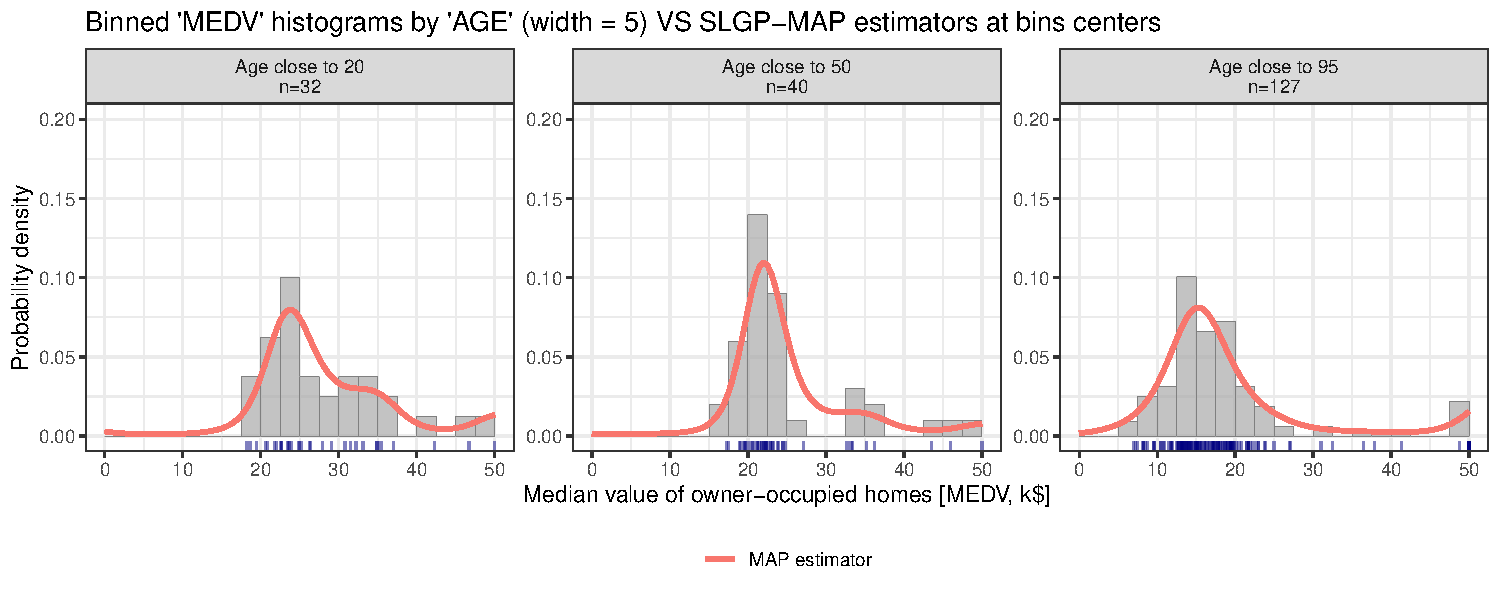
\includegraphics{IntroductionSLGP_files/figure-latex/SLGPplottingMAP-1} 

}

\caption{SLGP MAP versus histograms of median value at bins centered at several 'age' values}\label{fig:SLGPplottingMAP}
\end{figure}

\begin{Shaded}
\begin{Highlighting}[]

\FunctionTok{ggsave}\NormalTok{(}\FunctionTok{paste0}\NormalTok{(}\StringTok{"./Figures/histMAP"}\NormalTok{,  }\StringTok{".pdf"}\NormalTok{), }\AttributeTok{width=}\DecValTok{10}\NormalTok{, }\AttributeTok{height=}\DecValTok{5}\NormalTok{)}
\end{Highlighting}
\end{Shaded}

This other figure directly compares the SLGP MAP estimate to histograms of \texttt{medv} at selected \texttt{age} values, illustrating how well the model aligns with the observed data. Despite the small number of replicates, the SLGP estimate follows the empirical distribution, adapting to changes in shape across different age groups. The survivor bias is again visible, as the model assigns some probability mass to higher home values for older properties.

\subsubsection{Influence of the lengthscale selected}\label{influence-of-the-lengthscale-selected}

To assess the impact of lengthscale selection on SLGP estimation, we follow the MAP-based strategy described in the paper. We define a prior over the lengthscales, perform posterior evaluations over a regular grid, and compare optimization results under two different data usage regimes:

\begin{itemize}
\item
  Full dataset: model is trained and evaluated on the full data.
\item
  Partial training: model is trained on 25\% of the data and evaluated on the remaining 75\%.
\end{itemize}

Concretely, we specify an Inverse-Gamma prior on each lengthscale parameter.

\begin{Shaded}
\begin{Highlighting}[]
\FunctionTok{set.seed}\NormalTok{(}\DecValTok{1}\NormalTok{)}
\NormalTok{newOrder }\OtherTok{\textless{}{-}} \FunctionTok{sample}\NormalTok{(}\FunctionTok{seq}\NormalTok{(}\FunctionTok{nrow}\NormalTok{(df)))}

\NormalTok{dinvgamma }\OtherTok{\textless{}{-}} \ControlFlowTok{function}\NormalTok{(x, }\AttributeTok{alpha=}\FloatTok{4.5}\NormalTok{, }\AttributeTok{beta=}\FloatTok{0.35}\NormalTok{) \{}
  \FunctionTok{ifelse}\NormalTok{(x}\SpecialCharTok{\textless{}=}\DecValTok{0}\NormalTok{, }\DecValTok{0}\NormalTok{, (beta}\SpecialCharTok{\^{}}\NormalTok{alpha }\SpecialCharTok{/} \FunctionTok{gamma}\NormalTok{(alpha)) }\SpecialCharTok{*}\NormalTok{ x}\SpecialCharTok{\^{}}\NormalTok{(}\SpecialCharTok{{-}}\NormalTok{alpha }\SpecialCharTok{{-}} \DecValTok{1}\NormalTok{) }\SpecialCharTok{*} \FunctionTok{exp}\NormalTok{(}\SpecialCharTok{{-}}\NormalTok{beta }\SpecialCharTok{/}\NormalTok{ x))}
\NormalTok{\}}
\FunctionTok{plot}\NormalTok{(dinvgamma, }\AttributeTok{from=}\DecValTok{0}\NormalTok{, }\AttributeTok{to=}\DecValTok{1}\NormalTok{)}
\ControlFlowTok{if}\NormalTok{(}\FunctionTok{file.exists}\NormalTok{(}\StringTok{"OptimisingLen.RData"}\NormalTok{))\{}
  \FunctionTok{load}\NormalTok{(}\AttributeTok{file=}\StringTok{"OptimisingLen.RData"}\NormalTok{)}
  
\NormalTok{\}}\ControlFlowTok{else}\NormalTok{\{}
\NormalTok{  lengthscale\_grid }\OtherTok{\textless{}{-}} \FunctionTok{seq}\NormalTok{(}\FloatTok{0.025}\NormalTok{, }\FloatTok{0.5}\NormalTok{, }\FloatTok{0.025}\NormalTok{)}
\NormalTok{  df\_res }\OtherTok{\textless{}{-}} \FunctionTok{data.frame}\NormalTok{(}\FunctionTok{expand.grid}\NormalTok{(lengthscale\_grid, lengthscale\_grid))}
  \FunctionTok{colnames}\NormalTok{(df\_res) }\OtherTok{\textless{}{-}} \FunctionTok{c}\NormalTok{(}\StringTok{"l\_age"}\NormalTok{, }\StringTok{"l\_medv"}\NormalTok{)}
\NormalTok{  df\_res}\SpecialCharTok{$}\NormalTok{logPostData }\OtherTok{\textless{}{-}} \ConstantTok{NaN}
\NormalTok{  df\_res}\SpecialCharTok{$}\NormalTok{logPostData2 }\OtherTok{\textless{}{-}} \ConstantTok{NaN}
\NormalTok{\}}


\NormalTok{df\_res}\SpecialCharTok{$}\NormalTok{logPrior }\OtherTok{\textless{}{-}} \FunctionTok{log}\NormalTok{(}\FunctionTok{dinvgamma}\NormalTok{(df\_res}\SpecialCharTok{$}\NormalTok{l\_age))}\SpecialCharTok{+}\FunctionTok{log}\NormalTok{(}\FunctionTok{dinvgamma}\NormalTok{(df\_res}\SpecialCharTok{$}\NormalTok{l\_medv))}
\ControlFlowTok{for}\NormalTok{(i }\ControlFlowTok{in} \FunctionTok{which}\NormalTok{(}\FunctionTok{round}\NormalTok{(df\_res}\SpecialCharTok{$}\NormalTok{l\_age}\SpecialCharTok{*}\DecValTok{100}\NormalTok{)}\SpecialCharTok{\%\%}\DecValTok{5}\SpecialCharTok{==}\DecValTok{0}\SpecialCharTok{\&}
               \FunctionTok{round}\NormalTok{(df\_res}\SpecialCharTok{$}\NormalTok{l\_medv}\SpecialCharTok{*}\DecValTok{100}\NormalTok{)}\SpecialCharTok{\%\%}\DecValTok{5}\SpecialCharTok{==}\DecValTok{0}\NormalTok{))\{}
\NormalTok{  l1 }\OtherTok{\textless{}{-}}\NormalTok{ df\_res}\SpecialCharTok{$}\NormalTok{l\_age[i]}
\NormalTok{  l2 }\OtherTok{\textless{}{-}}\NormalTok{ df\_res}\SpecialCharTok{$}\NormalTok{l\_medv[i]}
  \ControlFlowTok{if}\NormalTok{(}\FunctionTok{is.na}\NormalTok{(df\_res}\SpecialCharTok{$}\NormalTok{logPostData[i]))\{}
    
\NormalTok{    modelMAPtemp }\OtherTok{\textless{}{-}} \FunctionTok{retrainSLGP}\NormalTok{(}\AttributeTok{SLGPmodel=}\NormalTok{modelMAP, }
                                \AttributeTok{newdata =}\NormalTok{ df, }
                                \AttributeTok{method=}\StringTok{"MAP"}\NormalTok{, }
                                \AttributeTok{hyperparams=}\FunctionTok{list}\NormalTok{(}\AttributeTok{sigma2=}\DecValTok{1}\NormalTok{, }
                                                 \AttributeTok{lengthscale=}\FunctionTok{c}\NormalTok{(l1, l2)),}
                                \AttributeTok{sigmaEstimationMethod=}\StringTok{"heuristic"}\NormalTok{)}
\NormalTok{    df\_res}\SpecialCharTok{$}\NormalTok{logPostData[i] }\OtherTok{\textless{}{-}}\NormalTok{ modelMAPtemp}\SpecialCharTok{@}\NormalTok{logPostData}
    \ControlFlowTok{if}\NormalTok{(}\FunctionTok{sum}\NormalTok{(}\SpecialCharTok{!}\FunctionTok{is.na}\NormalTok{(df\_res}\SpecialCharTok{$}\NormalTok{logPostData))}\SpecialCharTok{\%\%}\DecValTok{10}\SpecialCharTok{==}\DecValTok{0}\NormalTok{)\{}
      \FunctionTok{save}\NormalTok{(df\_res, }\AttributeTok{file=}\StringTok{"OptimisingLen.RData"}\NormalTok{)}
\NormalTok{    \}}
\NormalTok{  \}}
  \ControlFlowTok{if}\NormalTok{(}\FunctionTok{is.na}\NormalTok{(df\_res}\SpecialCharTok{$}\NormalTok{logPostData2[i]))\{}
    
\NormalTok{    modelMAPtemp }\OtherTok{\textless{}{-}} \FunctionTok{retrainSLGP}\NormalTok{(}\AttributeTok{SLGPmodel=}\NormalTok{modelMAP, }
                                \AttributeTok{newdata =}\NormalTok{ df[newOrder[}\DecValTok{1}\SpecialCharTok{:}\DecValTok{126}\NormalTok{], }
                                             \FunctionTok{c}\NormalTok{(}\StringTok{"age"}\NormalTok{, }\StringTok{"medv"}\NormalTok{)], }
                                \AttributeTok{method=}\StringTok{"MAP"}\NormalTok{, }
                                \AttributeTok{hyperparams=}\FunctionTok{list}\NormalTok{(}\AttributeTok{sigma2=}\DecValTok{1}\NormalTok{, }
                                                 \AttributeTok{lengthscale=}\FunctionTok{c}\NormalTok{(l1, l2)),}
                                \AttributeTok{sigmaEstimationMethod=}\StringTok{"heuristic"}\NormalTok{)}
\NormalTok{    temp }\OtherTok{\textless{}{-}} \FunctionTok{predictSLGP\_newNode}\NormalTok{(modelMAPtemp,}
                                \AttributeTok{newNodes =}\NormalTok{ df[newOrder[}\SpecialCharTok{{-}}\FunctionTok{c}\NormalTok{(}\DecValTok{1}\SpecialCharTok{:}\DecValTok{126}\NormalTok{)], }
                                              \FunctionTok{c}\NormalTok{(}\StringTok{"age"}\NormalTok{, }\StringTok{"medv"}\NormalTok{) ])}
\NormalTok{    df\_res}\SpecialCharTok{$}\NormalTok{logPostData2[i] }\OtherTok{\textless{}{-}} \FunctionTok{sum}\NormalTok{(}\FunctionTok{log}\NormalTok{(temp}\SpecialCharTok{$}\NormalTok{pdf\_1))}
    \ControlFlowTok{if}\NormalTok{(}\FunctionTok{sum}\NormalTok{(}\SpecialCharTok{!}\FunctionTok{is.na}\NormalTok{(df\_res}\SpecialCharTok{$}\NormalTok{logPostData2))}\SpecialCharTok{\%\%}\DecValTok{10}\SpecialCharTok{==}\DecValTok{0}\NormalTok{)\{}
      \FunctionTok{save}\NormalTok{(df\_res, }\AttributeTok{file=}\StringTok{"OptimisingLen.RData"}\NormalTok{)}
\NormalTok{    \}}
\NormalTok{  \}}
\NormalTok{\}}
\FunctionTok{save}\NormalTok{(df\_res, }\AttributeTok{file=}\StringTok{"OptimisingLen.RData"}\NormalTok{)}
\end{Highlighting}
\end{Shaded}

The following figure displays the resulting posterior landscapes.

\begin{Shaded}
\begin{Highlighting}[]
\FunctionTok{load}\NormalTok{(}\AttributeTok{file=}\StringTok{"OptimisingLen.RData"}\NormalTok{)}

\NormalTok{min1 }\OtherTok{\textless{}{-}}\NormalTok{ df\_res[}\FunctionTok{which.min}\NormalTok{(}\SpecialCharTok{{-}}\NormalTok{df\_res}\SpecialCharTok{$}\NormalTok{logPostData}\SpecialCharTok{{-}}\NormalTok{df\_res}\SpecialCharTok{$}\NormalTok{logPrior), ]}
\NormalTok{min2 }\OtherTok{\textless{}{-}}\NormalTok{ df\_res[}\FunctionTok{which.min}\NormalTok{(}\SpecialCharTok{{-}}\NormalTok{df\_res}\SpecialCharTok{$}\NormalTok{logPostData2}\SpecialCharTok{{-}}\NormalTok{df\_res}\SpecialCharTok{$}\NormalTok{logPrior), ]}
\NormalTok{plot1 }\OtherTok{\textless{}{-}}\NormalTok{ df\_res }\SpecialCharTok{\%\textgreater{}\%}
\NormalTok{  dplyr}\SpecialCharTok{::}\FunctionTok{filter}\NormalTok{(}\SpecialCharTok{!}\FunctionTok{is.na}\NormalTok{(logPostData))}\SpecialCharTok{\%\textgreater{}\%}
  \FunctionTok{ggplot}\NormalTok{(}\AttributeTok{mapping=}\FunctionTok{aes}\NormalTok{(}\AttributeTok{x=}\NormalTok{l\_age, }\AttributeTok{y=}\NormalTok{l\_medv))}\SpecialCharTok{+}
  \FunctionTok{geom\_tile}\NormalTok{(}\AttributeTok{mapping=}\FunctionTok{aes}\NormalTok{(}\AttributeTok{fill=}\SpecialCharTok{{-}}\NormalTok{logPostData}\SpecialCharTok{{-}}\NormalTok{logPrior))}\SpecialCharTok{+}
  \FunctionTok{geom\_contour}\NormalTok{(}\AttributeTok{mapping=}\FunctionTok{aes}\NormalTok{(}\AttributeTok{z=}\SpecialCharTok{{-}}\NormalTok{logPostData}\SpecialCharTok{{-}}\NormalTok{logPrior), }\AttributeTok{col=}\StringTok{"black"}\NormalTok{, }\AttributeTok{bins=}\DecValTok{20}\NormalTok{)}\SpecialCharTok{+}
  \FunctionTok{geom\_point}\NormalTok{(}\AttributeTok{data=}\NormalTok{min1, }\AttributeTok{col=}\StringTok{"red"}\NormalTok{)}\SpecialCharTok{+}
  \FunctionTok{theme\_bw}\NormalTok{()}\SpecialCharTok{+}
  \FunctionTok{scale\_fill\_viridis}\NormalTok{(}\AttributeTok{direction=}\SpecialCharTok{{-}}\DecValTok{1}\NormalTok{)}\SpecialCharTok{+}
  \FunctionTok{labs}\NormalTok{(}\AttributeTok{fill=}\StringTok{"log Posterior"}\NormalTok{)}\SpecialCharTok{+}
  \FunctionTok{theme}\NormalTok{(}\AttributeTok{legend.position =} \StringTok{"bottom"}\NormalTok{,}
        \AttributeTok{legend.direction=}\StringTok{"horizontal"}\NormalTok{)}\SpecialCharTok{+}
  \FunctionTok{ggtitle}\NormalTok{(}\StringTok{"Trained and evaluated on full dataset."}\NormalTok{)}

\NormalTok{plot2 }\OtherTok{\textless{}{-}}\NormalTok{ df\_res }\SpecialCharTok{\%\textgreater{}\%}
\NormalTok{  dplyr}\SpecialCharTok{::}\FunctionTok{filter}\NormalTok{(}\SpecialCharTok{!}\FunctionTok{is.na}\NormalTok{(logPostData2))}\SpecialCharTok{\%\textgreater{}\%}
  \FunctionTok{ggplot}\NormalTok{(}\AttributeTok{mapping=}\FunctionTok{aes}\NormalTok{(}\AttributeTok{x=}\NormalTok{l\_age, }\AttributeTok{y=}\NormalTok{l\_medv))}\SpecialCharTok{+}
  \FunctionTok{geom\_tile}\NormalTok{(}\AttributeTok{mapping=}\FunctionTok{aes}\NormalTok{(}\AttributeTok{fill=}\SpecialCharTok{{-}}\NormalTok{logPostData2}\SpecialCharTok{{-}}\NormalTok{logPrior))}\SpecialCharTok{+}
  \FunctionTok{geom\_contour}\NormalTok{(}\AttributeTok{mapping=}\FunctionTok{aes}\NormalTok{(}\AttributeTok{z=}\SpecialCharTok{{-}}\NormalTok{logPostData2}\SpecialCharTok{{-}}\NormalTok{logPrior), }\AttributeTok{col=}\StringTok{"black"}\NormalTok{, }\AttributeTok{bins=}\DecValTok{20}\NormalTok{)}\SpecialCharTok{+}
  \FunctionTok{geom\_point}\NormalTok{(}\AttributeTok{data=}\NormalTok{min2, }\AttributeTok{col=}\StringTok{"red"}\NormalTok{)}\SpecialCharTok{+}
  \FunctionTok{theme\_bw}\NormalTok{()}\SpecialCharTok{+}
  \FunctionTok{scale\_fill\_viridis}\NormalTok{(}\AttributeTok{direction=}\SpecialCharTok{{-}}\DecValTok{1}\NormalTok{)}\SpecialCharTok{+}
  \FunctionTok{labs}\NormalTok{(}\AttributeTok{fill=}\StringTok{"log Posterior"}\NormalTok{)}\SpecialCharTok{+}
  \FunctionTok{theme}\NormalTok{(}\AttributeTok{legend.position =} \StringTok{"bottom"}\NormalTok{,}
        \AttributeTok{legend.direction=}\StringTok{"horizontal"}\NormalTok{)}\SpecialCharTok{+}
  \FunctionTok{ggtitle}\NormalTok{(}\StringTok{"Trained on 1/4 of dataset, evaluated on the rest."}\NormalTok{)}

\FunctionTok{library}\NormalTok{(ggpubr)}

\FunctionTok{ggarrange}\NormalTok{(plot1, plot2)}
\end{Highlighting}
\end{Shaded}

\begin{figure}[H]

{\centering 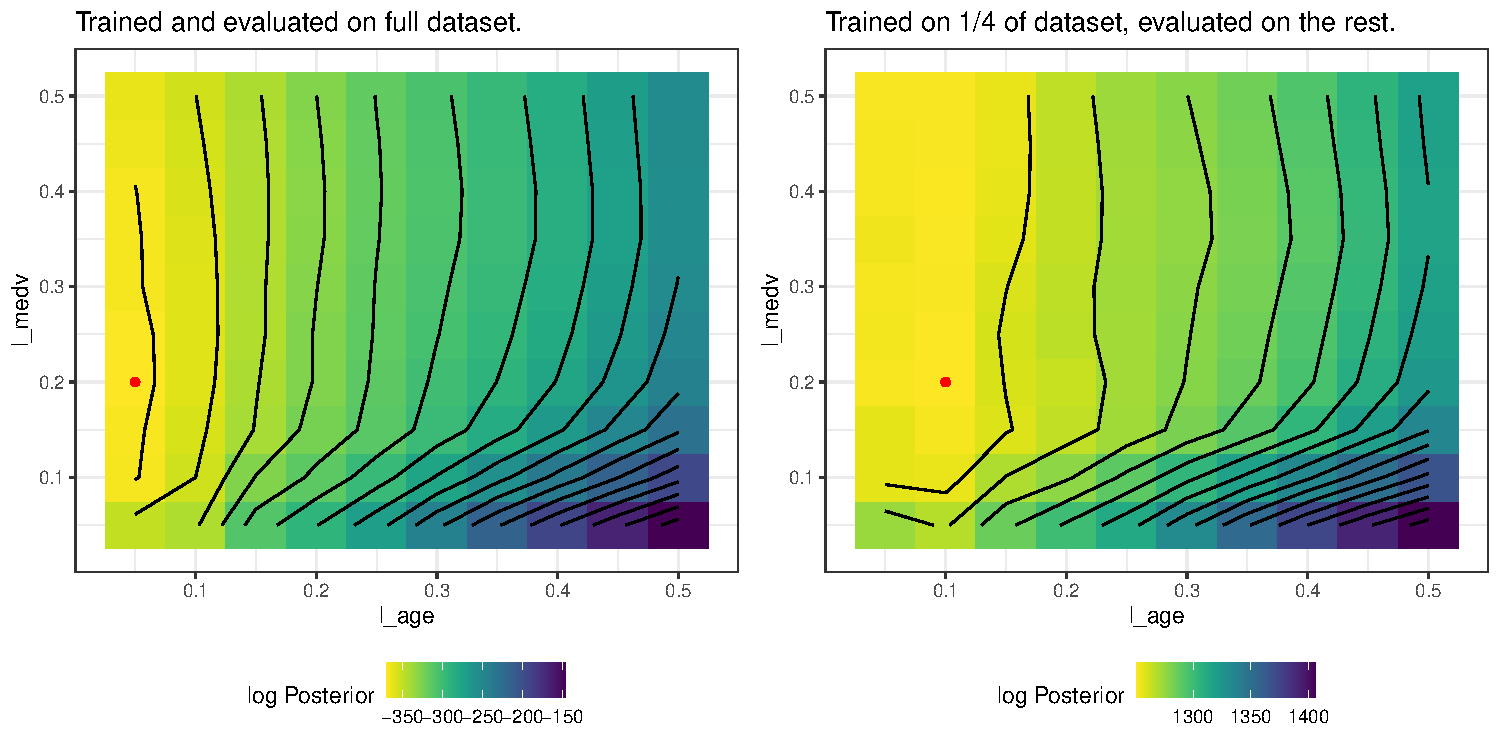
\includegraphics{IntroductionSLGP_files/figure-latex/optimlandscape-1} 

}

\caption{Posterior log-density (up to a constant) over the lengthscale grid (age, medv), under two training strategies. Left: trained and evaluated on the full dataset. Right trained on 25\% of the data, evaluated on the remaining 75\%. The red dot indicates the optimal lengthscales in each setting.}\label{fig:optimlandscape}
\end{figure}

We observe that:

\begin{itemize}
\item
  Both approaches yield similar optimal lengthscales, showing the stability of the selection.
\item
  These landscapes are fairly consistent with our proposed heuristic of setting all lengthscales around 10-15\% of the ranges.
\end{itemize}

Now, for a qualitative intepretation, we fit and compare SLGP models with three representative choices of lengthscales:

\begin{itemize}
\item
  Short lengthscales \((0.01, 0.01)\) --- inducing highly localized priors,
\item
  Long lengthscales \((0.5, 0.5)\) --- yielding overly smooth priors,
\item
  Data-driven MAP estimate from the partial training scheme.
\end{itemize}

\begin{Shaded}
\begin{Highlighting}[]
\CommentTok{\# Or equivalent, re{-}use the same basis functions }
\CommentTok{\# and hyper parameters as in the prior we saw}

\NormalTok{modelMAP2 }\OtherTok{\textless{}{-}} \FunctionTok{retrainSLGP}\NormalTok{(}\AttributeTok{SLGPmodel=}\NormalTok{modelPrior, }
                         \AttributeTok{newdata =}\NormalTok{ df, }
                         \AttributeTok{method=}\StringTok{"MAP"}\NormalTok{, }
                         \AttributeTok{hyperparams=}\FunctionTok{list}\NormalTok{(}\AttributeTok{sigma2=}\DecValTok{1}\NormalTok{, }
                                          \AttributeTok{lengthscale=}\FunctionTok{c}\NormalTok{(}\FloatTok{0.01}\NormalTok{, }\FloatTok{0.01}\NormalTok{)),}
                         \AttributeTok{sigmaEstimationMethod=}\StringTok{"heuristic"}\NormalTok{)}
\NormalTok{modelMAP3 }\OtherTok{\textless{}{-}} \FunctionTok{retrainSLGP}\NormalTok{(}\AttributeTok{SLGPmodel=}\NormalTok{modelPrior, }
                         \AttributeTok{newdata =}\NormalTok{ df, }
                         \AttributeTok{method=}\StringTok{"MAP"}\NormalTok{, }
                         \AttributeTok{hyperparams=}\FunctionTok{list}\NormalTok{(}\AttributeTok{sigma2=}\DecValTok{1}\NormalTok{, }
                                          \AttributeTok{lengthscale=}\FunctionTok{c}\NormalTok{(}\FloatTok{0.5}\NormalTok{, }\FloatTok{0.5}\NormalTok{)),}
                         \AttributeTok{sigmaEstimationMethod=}\StringTok{"heuristic"}\NormalTok{)}
\NormalTok{modelMAP4 }\OtherTok{\textless{}{-}} \FunctionTok{retrainSLGP}\NormalTok{(}\AttributeTok{SLGPmodel=}\NormalTok{modelPrior, }
                         \AttributeTok{newdata =}\NormalTok{ df, }
                         \AttributeTok{method=}\StringTok{"MAP"}\NormalTok{, }
                         \AttributeTok{hyperparams=}\FunctionTok{list}\NormalTok{(}\AttributeTok{sigma2=}\DecValTok{1}\NormalTok{, }
                                          \AttributeTok{lengthscale=}\FunctionTok{c}\NormalTok{(min2}\SpecialCharTok{$}\NormalTok{l\_medv, min2}\SpecialCharTok{$}\NormalTok{l\_age)),}
                         \AttributeTok{sigmaEstimationMethod=}\StringTok{"heuristic"}\NormalTok{)}
\FunctionTok{gc}\NormalTok{()}
\CommentTok{\#\textgreater{}           used  (Mb) gc trigger  (Mb) max used  (Mb)}
\CommentTok{\#\textgreater{} Ncells 2281950 121.9    4691755 250.6  4691755 250.6}
\CommentTok{\#\textgreater{} Vcells 6766005  51.7   23662044 180.6 28201788 215.2}
\end{Highlighting}
\end{Shaded}

This results in the following fitted densities:

\begin{Shaded}
\begin{Highlighting}[]
\NormalTok{dfGrid }\OtherTok{\textless{}{-}} \FunctionTok{data.frame}\NormalTok{(}\FunctionTok{expand.grid}\NormalTok{(}\FunctionTok{seq}\NormalTok{(range\_x[}\DecValTok{1}\NormalTok{], range\_x[}\DecValTok{2}\NormalTok{], }\DecValTok{5}\NormalTok{), }
                                 \FunctionTok{seq}\NormalTok{(range\_response[}\DecValTok{1}\NormalTok{], range\_response[}\DecValTok{2}\NormalTok{],, }\DecValTok{101}\NormalTok{)))}
\FunctionTok{colnames}\NormalTok{(dfGrid) }\OtherTok{\textless{}{-}} \FunctionTok{c}\NormalTok{(}\StringTok{"age"}\NormalTok{, }\StringTok{"medv"}\NormalTok{)}
\NormalTok{pred1 }\OtherTok{\textless{}{-}} \FunctionTok{predictSLGP\_newNode}\NormalTok{(}\AttributeTok{SLGPmodel=}\NormalTok{modelMAP,}
                             \AttributeTok{newNodes =}\NormalTok{ dfGrid)}
\NormalTok{pred1}\SpecialCharTok{$}\NormalTok{Len }\OtherTok{\textless{}{-}} \StringTok{"Heuristic lengthscale"}
\NormalTok{pred2 }\OtherTok{\textless{}{-}} \FunctionTok{predictSLGP\_newNode}\NormalTok{(}\AttributeTok{SLGPmodel=}\NormalTok{modelMAP2,}
                             \AttributeTok{newNodes =}\NormalTok{ dfGrid)}
\NormalTok{pred2}\SpecialCharTok{$}\NormalTok{Len }\OtherTok{\textless{}{-}} \StringTok{"Short lengthscale"}
\NormalTok{pred3 }\OtherTok{\textless{}{-}} \FunctionTok{predictSLGP\_newNode}\NormalTok{(}\AttributeTok{SLGPmodel=}\NormalTok{modelMAP3,}
                             \AttributeTok{newNodes =}\NormalTok{ dfGrid)}
\NormalTok{pred3}\SpecialCharTok{$}\NormalTok{Len }\OtherTok{\textless{}{-}} \StringTok{"Long lengthscale"}
\NormalTok{pred4 }\OtherTok{\textless{}{-}} \FunctionTok{predictSLGP\_newNode}\NormalTok{(}\AttributeTok{SLGPmodel=}\NormalTok{modelMAP4,}
                             \AttributeTok{newNodes =}\NormalTok{ dfGrid)}
\NormalTok{pred4}\SpecialCharTok{$}\NormalTok{Len }\OtherTok{\textless{}{-}} \StringTok{"Optimised lengthscale"}
\NormalTok{pred }\OtherTok{\textless{}{-}} \FunctionTok{rbind}\NormalTok{(pred1, pred2, pred3, pred4)}
\NormalTok{scale\_factor }\OtherTok{\textless{}{-}} \DecValTok{100}
\FunctionTok{ggplot}\NormalTok{()  }\SpecialCharTok{+}
  \FunctionTok{labs}\NormalTok{(}\AttributeTok{y =} \StringTok{"Proportion of owner{-}occupied units}\SpecialCharTok{\textbackslash{}n}\StringTok{built prior to 1940 [\%]"}\NormalTok{, }
       \AttributeTok{x =} \StringTok{"Median value of owner{-}occupied homes [k$]"}\NormalTok{,}
       \AttributeTok{title =} \StringTok{"Median value vs. age of homes"}\NormalTok{) }\SpecialCharTok{+}
  \FunctionTok{theme\_bw}\NormalTok{()}\SpecialCharTok{+}
  \FunctionTok{geom\_ribbon}\NormalTok{(}\AttributeTok{data=}\NormalTok{pred,}
              \AttributeTok{mapping=}\FunctionTok{aes}\NormalTok{(}\AttributeTok{x=}\NormalTok{medv, }\AttributeTok{ymax=}\NormalTok{scale\_factor}\SpecialCharTok{*}\NormalTok{pdf\_1}\SpecialCharTok{+}\NormalTok{age, }
                          \AttributeTok{ymin=}\NormalTok{age, }\AttributeTok{group=}\SpecialCharTok{{-}}\NormalTok{age, }\AttributeTok{fill=}\NormalTok{age),}
              \AttributeTok{col=}\StringTok{"grey"}\NormalTok{, }\AttributeTok{alpha=}\FloatTok{0.9}\NormalTok{)}\SpecialCharTok{+}
  \FunctionTok{geom\_point}\NormalTok{(}\AttributeTok{data=}\NormalTok{df,}
             \AttributeTok{mapping=}\FunctionTok{aes}\NormalTok{(}\AttributeTok{x =}\NormalTok{ medv, }\AttributeTok{y =}\NormalTok{ age), }\AttributeTok{alpha =} \FloatTok{0.5}\NormalTok{, }\AttributeTok{color =} \StringTok{"navy"}\NormalTok{)}\SpecialCharTok{+}
  \FunctionTok{scale\_fill\_viridis}\NormalTok{(}\AttributeTok{option =} \StringTok{"plasma"}\NormalTok{,}
                     \AttributeTok{guide =} \FunctionTok{guide\_colorbar}\NormalTok{(}\AttributeTok{nrow =} \DecValTok{1}\NormalTok{,}
                                            \AttributeTok{title =} \StringTok{"Indexing variable: }
\StringTok{                                            Proportion of owner{-}occupied units built }
\StringTok{                                            prior to 1940"}\NormalTok{,}
                                            \AttributeTok{barheight =} \FunctionTok{unit}\NormalTok{(}\DecValTok{2}\NormalTok{, }\AttributeTok{units =} \StringTok{"mm"}\NormalTok{),}
                                            \AttributeTok{barwidth =} \FunctionTok{unit}\NormalTok{(}\DecValTok{55}\NormalTok{, }\AttributeTok{units =} \StringTok{"mm"}\NormalTok{),}
                                            \AttributeTok{title.position =} \StringTok{\textquotesingle{}top\textquotesingle{}}\NormalTok{,}
                                            \AttributeTok{label.position =} \StringTok{"bottom"}\NormalTok{,}
                                            \AttributeTok{title.hjust =} \FloatTok{0.5}\NormalTok{))}\SpecialCharTok{+}
  \FunctionTok{theme}\NormalTok{(}\AttributeTok{legend.position =} \StringTok{"bottom"}\NormalTok{)}\SpecialCharTok{+}
  \FunctionTok{facet\_grid}\NormalTok{(Len}\SpecialCharTok{\textasciitilde{}}\NormalTok{.)}\SpecialCharTok{+}
  \FunctionTok{coord\_flip}\NormalTok{()}
\end{Highlighting}
\end{Shaded}

\begin{figure}[H]

{\centering 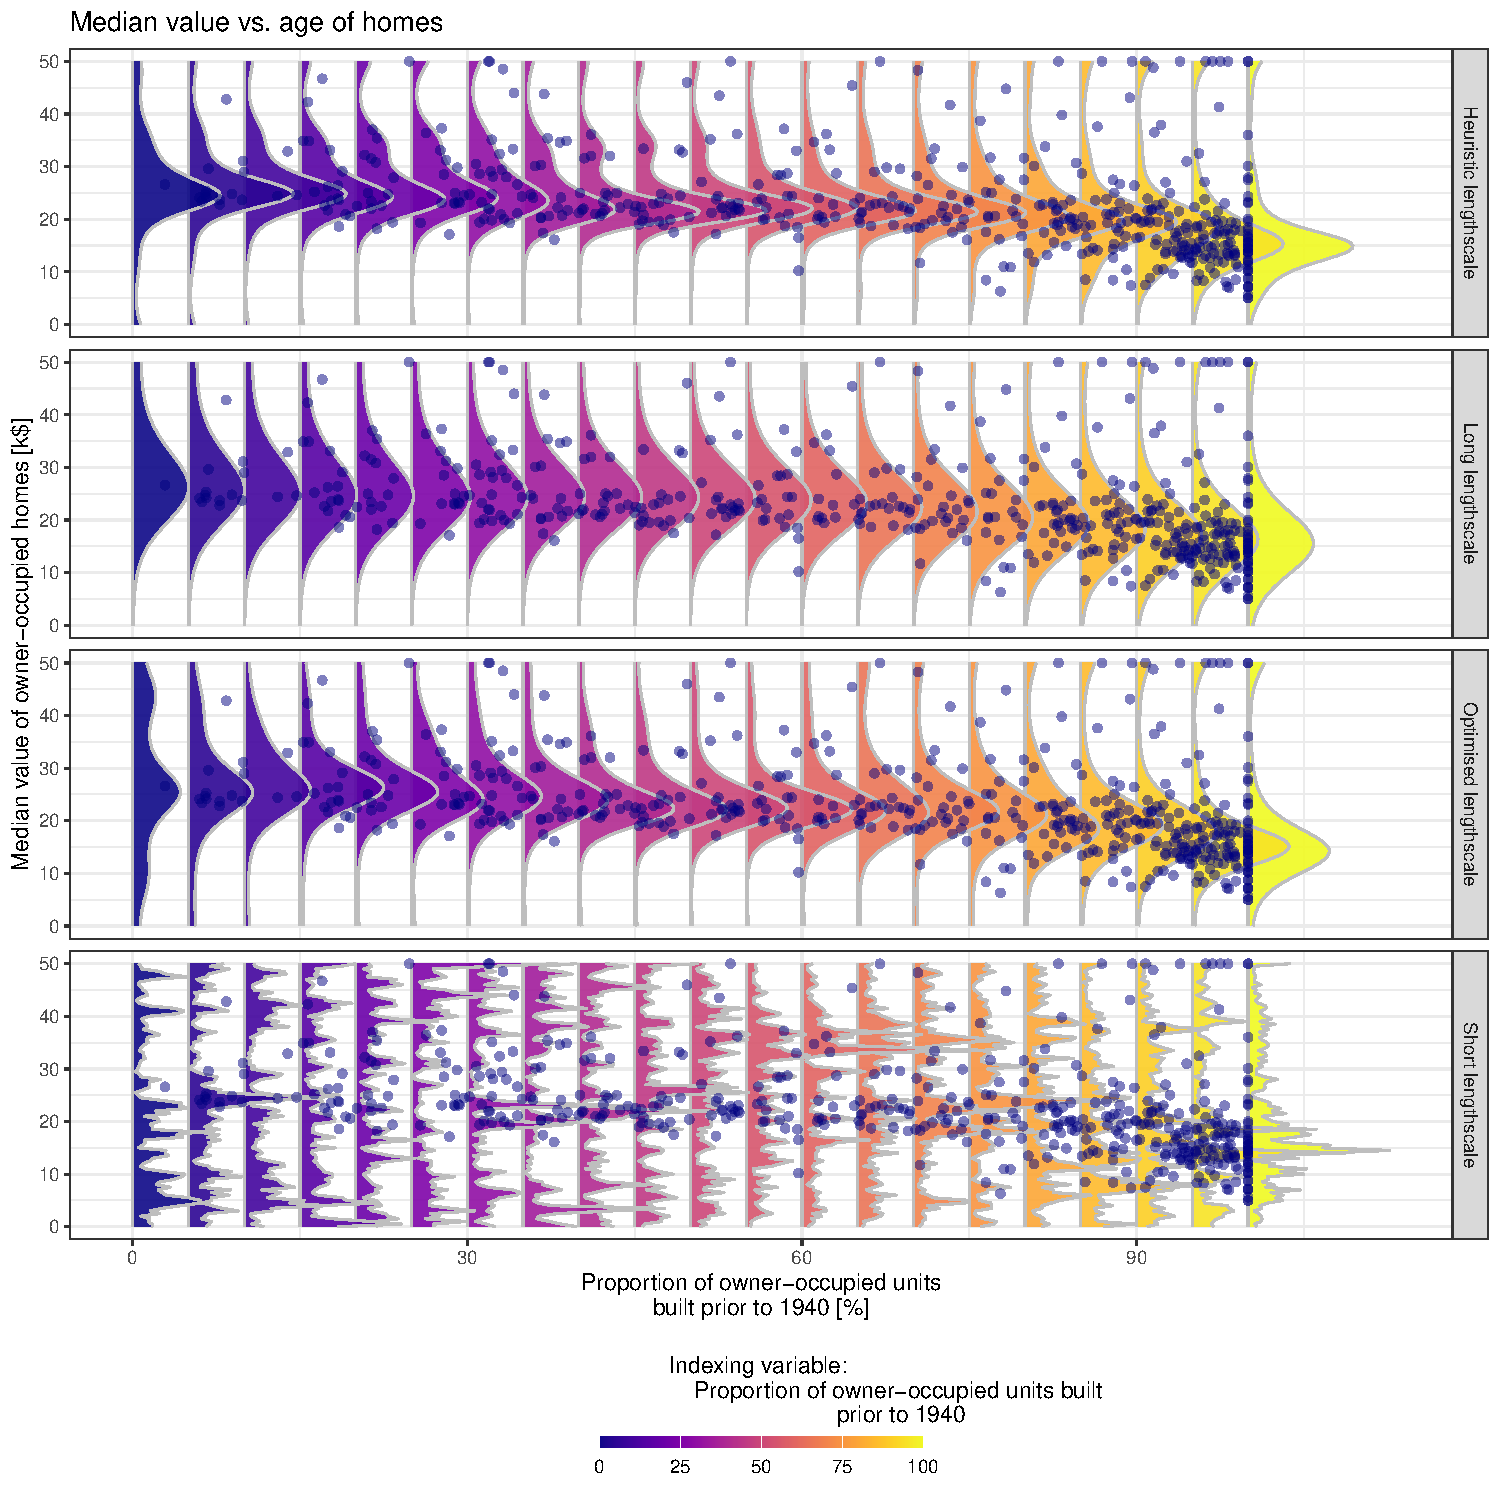
\includegraphics{IntroductionSLGP_files/figure-latex/plotRibbonsLen1-1} 

}

\caption{Comparison of fitted densities under different lengthscale settings}\label{fig:plotRibbonsLen1}
\end{figure}

\begin{Shaded}
\begin{Highlighting}[]
\NormalTok{dfGrid }\OtherTok{\textless{}{-}} \FunctionTok{data.frame}\NormalTok{(}\FunctionTok{expand.grid}\NormalTok{(}\FunctionTok{seq}\NormalTok{(range\_x[}\DecValTok{1}\NormalTok{], range\_x[}\DecValTok{2}\NormalTok{], }\DecValTok{5}\NormalTok{), }
                                 \FunctionTok{seq}\NormalTok{(range\_response[}\DecValTok{1}\NormalTok{], range\_response[}\DecValTok{2}\NormalTok{],, }\DecValTok{101}\NormalTok{)))}
\FunctionTok{colnames}\NormalTok{(dfGrid) }\OtherTok{\textless{}{-}} \FunctionTok{c}\NormalTok{(}\StringTok{"age"}\NormalTok{, }\StringTok{"medv"}\NormalTok{)}

\NormalTok{dfGrid }\OtherTok{\textless{}{-}} \FunctionTok{data.frame}\NormalTok{(}\FunctionTok{expand.grid}\NormalTok{(selected\_values, }
                                 \FunctionTok{seq}\NormalTok{(range\_response[}\DecValTok{1}\NormalTok{], range\_response[}\DecValTok{2}\NormalTok{],, }\DecValTok{101}\NormalTok{)))}
\FunctionTok{colnames}\NormalTok{(dfGrid) }\OtherTok{\textless{}{-}} \FunctionTok{c}\NormalTok{(}\StringTok{"age"}\NormalTok{, }\StringTok{"medv"}\NormalTok{)}
\NormalTok{pred1 }\OtherTok{\textless{}{-}} \FunctionTok{predictSLGP\_newNode}\NormalTok{(}\AttributeTok{SLGPmodel=}\NormalTok{modelMAP,}
                             \AttributeTok{newNodes =}\NormalTok{ dfGrid)}
\NormalTok{pred1}\SpecialCharTok{$}\NormalTok{Len }\OtherTok{\textless{}{-}} \StringTok{"Heuristic lengthscale"}
\NormalTok{pred2 }\OtherTok{\textless{}{-}} \FunctionTok{predictSLGP\_newNode}\NormalTok{(}\AttributeTok{SLGPmodel=}\NormalTok{modelMAP2,}
                             \AttributeTok{newNodes =}\NormalTok{ dfGrid)}
\NormalTok{pred2}\SpecialCharTok{$}\NormalTok{Len }\OtherTok{\textless{}{-}} \StringTok{"Short lengthscale"}
\NormalTok{pred3 }\OtherTok{\textless{}{-}} \FunctionTok{predictSLGP\_newNode}\NormalTok{(}\AttributeTok{SLGPmodel=}\NormalTok{modelMAP3,}
                             \AttributeTok{newNodes =}\NormalTok{ dfGrid)}
\NormalTok{pred3}\SpecialCharTok{$}\NormalTok{Len }\OtherTok{\textless{}{-}} \StringTok{"Long lengthscale"}
\NormalTok{pred4 }\OtherTok{\textless{}{-}} \FunctionTok{predictSLGP\_newNode}\NormalTok{(}\AttributeTok{SLGPmodel=}\NormalTok{modelMAP4,}
                             \AttributeTok{newNodes =}\NormalTok{ dfGrid)}
\NormalTok{pred4}\SpecialCharTok{$}\NormalTok{Len }\OtherTok{\textless{}{-}} \StringTok{"Optimised lengthscale"}
\NormalTok{pred }\OtherTok{\textless{}{-}} \FunctionTok{rbind}\NormalTok{(pred1, pred2, pred3, pred4)}
\FunctionTok{colnames}\NormalTok{(pred) }\OtherTok{\textless{}{-}} \FunctionTok{c}\NormalTok{(}\StringTok{"age"}\NormalTok{, }\StringTok{"medv"}\NormalTok{, }\StringTok{"MAP estimator"}\NormalTok{, }\StringTok{"Len"}\NormalTok{)}
\NormalTok{pred }\OtherTok{\textless{}{-}}\NormalTok{ pred}\SpecialCharTok{\%\textgreater{}\%}
  \FunctionTok{pivot\_longer}\NormalTok{(}\SpecialCharTok{{-}}\FunctionTok{c}\NormalTok{(}\StringTok{"age"}\NormalTok{, }\StringTok{"medv"}\NormalTok{, }\StringTok{"Len"}\NormalTok{))}
\NormalTok{pred}\SpecialCharTok{$}\NormalTok{category }\OtherTok{\textless{}{-}}\FunctionTok{ifelse}\NormalTok{(pred}\SpecialCharTok{$}\NormalTok{age}\SpecialCharTok{==}\NormalTok{selected\_values[}\DecValTok{1}\NormalTok{], names[}\DecValTok{1}\NormalTok{],}
                          \FunctionTok{ifelse}\NormalTok{(pred}\SpecialCharTok{$}\NormalTok{age}\SpecialCharTok{==}\NormalTok{selected\_values[}\DecValTok{2}\NormalTok{], names[}\DecValTok{2}\NormalTok{], names[}\DecValTok{3}\NormalTok{]))}

\FunctionTok{ggplot}\NormalTok{(}\AttributeTok{mapping=}\FunctionTok{aes}\NormalTok{(}\AttributeTok{x =}\NormalTok{ medv)) }\SpecialCharTok{+}
  \FunctionTok{geom\_histogram}\NormalTok{(df\_filtered,}
                 \AttributeTok{mapping=}\FunctionTok{aes}\NormalTok{(}\AttributeTok{y=}\FunctionTok{after\_stat}\NormalTok{(density)),}
                 \AttributeTok{position =} \StringTok{"identity"}\NormalTok{, }\AttributeTok{breaks =} \FunctionTok{seq}\NormalTok{(}\DecValTok{0}\NormalTok{, }\DecValTok{50}\NormalTok{, }\FloatTok{2.5}\NormalTok{),}
                 \AttributeTok{fill=}\StringTok{"darkgrey"}\NormalTok{, }\AttributeTok{col=}\StringTok{"grey50"}\NormalTok{, }\AttributeTok{lwd=}\FloatTok{0.2}\NormalTok{, }\AttributeTok{alpha=}\FloatTok{0.7}\NormalTok{) }\SpecialCharTok{+}
  \FunctionTok{geom\_rug}\NormalTok{(}\AttributeTok{data=}\NormalTok{df\_filtered, }\AttributeTok{sides =} \StringTok{"b"}\NormalTok{, }\AttributeTok{color =} \StringTok{"navy"}\NormalTok{, }\AttributeTok{alpha =} \FloatTok{0.5}\NormalTok{)}\SpecialCharTok{+}
  \FunctionTok{geom\_line}\NormalTok{(}\AttributeTok{data=}\NormalTok{pred, }\AttributeTok{mapping=}\FunctionTok{aes}\NormalTok{(}\AttributeTok{y=}\NormalTok{value, }\AttributeTok{group=}\NormalTok{name), }
            \AttributeTok{color =} \StringTok{"black"}\NormalTok{, }\AttributeTok{lwd=}\FloatTok{0.1}\NormalTok{, }\AttributeTok{alpha=}\FloatTok{0.5}\NormalTok{)}\SpecialCharTok{+}
  \FunctionTok{geom\_line}\NormalTok{(}\AttributeTok{data=}\NormalTok{pred, }\AttributeTok{mapping=}\FunctionTok{aes}\NormalTok{(}\AttributeTok{y=}\NormalTok{value, }\AttributeTok{group=}\NormalTok{name, }\AttributeTok{col=}\NormalTok{name), }\AttributeTok{lwd=}\FloatTok{1.1}\NormalTok{)}\SpecialCharTok{+}
  \FunctionTok{facet\_grid}\NormalTok{(Len }\SpecialCharTok{\textasciitilde{}}\NormalTok{ category, }\AttributeTok{scales =} \StringTok{"free\_y"}\NormalTok{) }\SpecialCharTok{+}
  \FunctionTok{labs}\NormalTok{(}\AttributeTok{x =} \StringTok{"Median value of owner{-}occupied homes [k$]"}\NormalTok{, }
       \AttributeTok{y =} \StringTok{"Probability density"}\NormalTok{, }
       \AttributeTok{title =} \StringTok{"Histogram of median value at bins centered at several \textquotesingle{}age\textquotesingle{} values, with width 5}\SpecialCharTok{\textbackslash{}n}\StringTok{versus draws from a SLGP prior"}\NormalTok{) }\SpecialCharTok{+}
  \FunctionTok{theme\_bw}\NormalTok{()}\SpecialCharTok{+}
  \FunctionTok{theme}\NormalTok{(}\AttributeTok{legend.position=}\StringTok{"bottom"}\NormalTok{,}
        \AttributeTok{legend.direction =} \StringTok{"horizontal"}\NormalTok{,}
        \AttributeTok{legend.title =} \FunctionTok{element\_blank}\NormalTok{())}\SpecialCharTok{+}
  \FunctionTok{coord\_cartesian}\NormalTok{(}\AttributeTok{xlim=}\NormalTok{range\_response,}
                  \AttributeTok{ylim=}\FunctionTok{c}\NormalTok{(}\DecValTok{0}\NormalTok{, }\FloatTok{0.25}\NormalTok{))}
\end{Highlighting}
\end{Shaded}

\begin{figure}[H]

{\centering 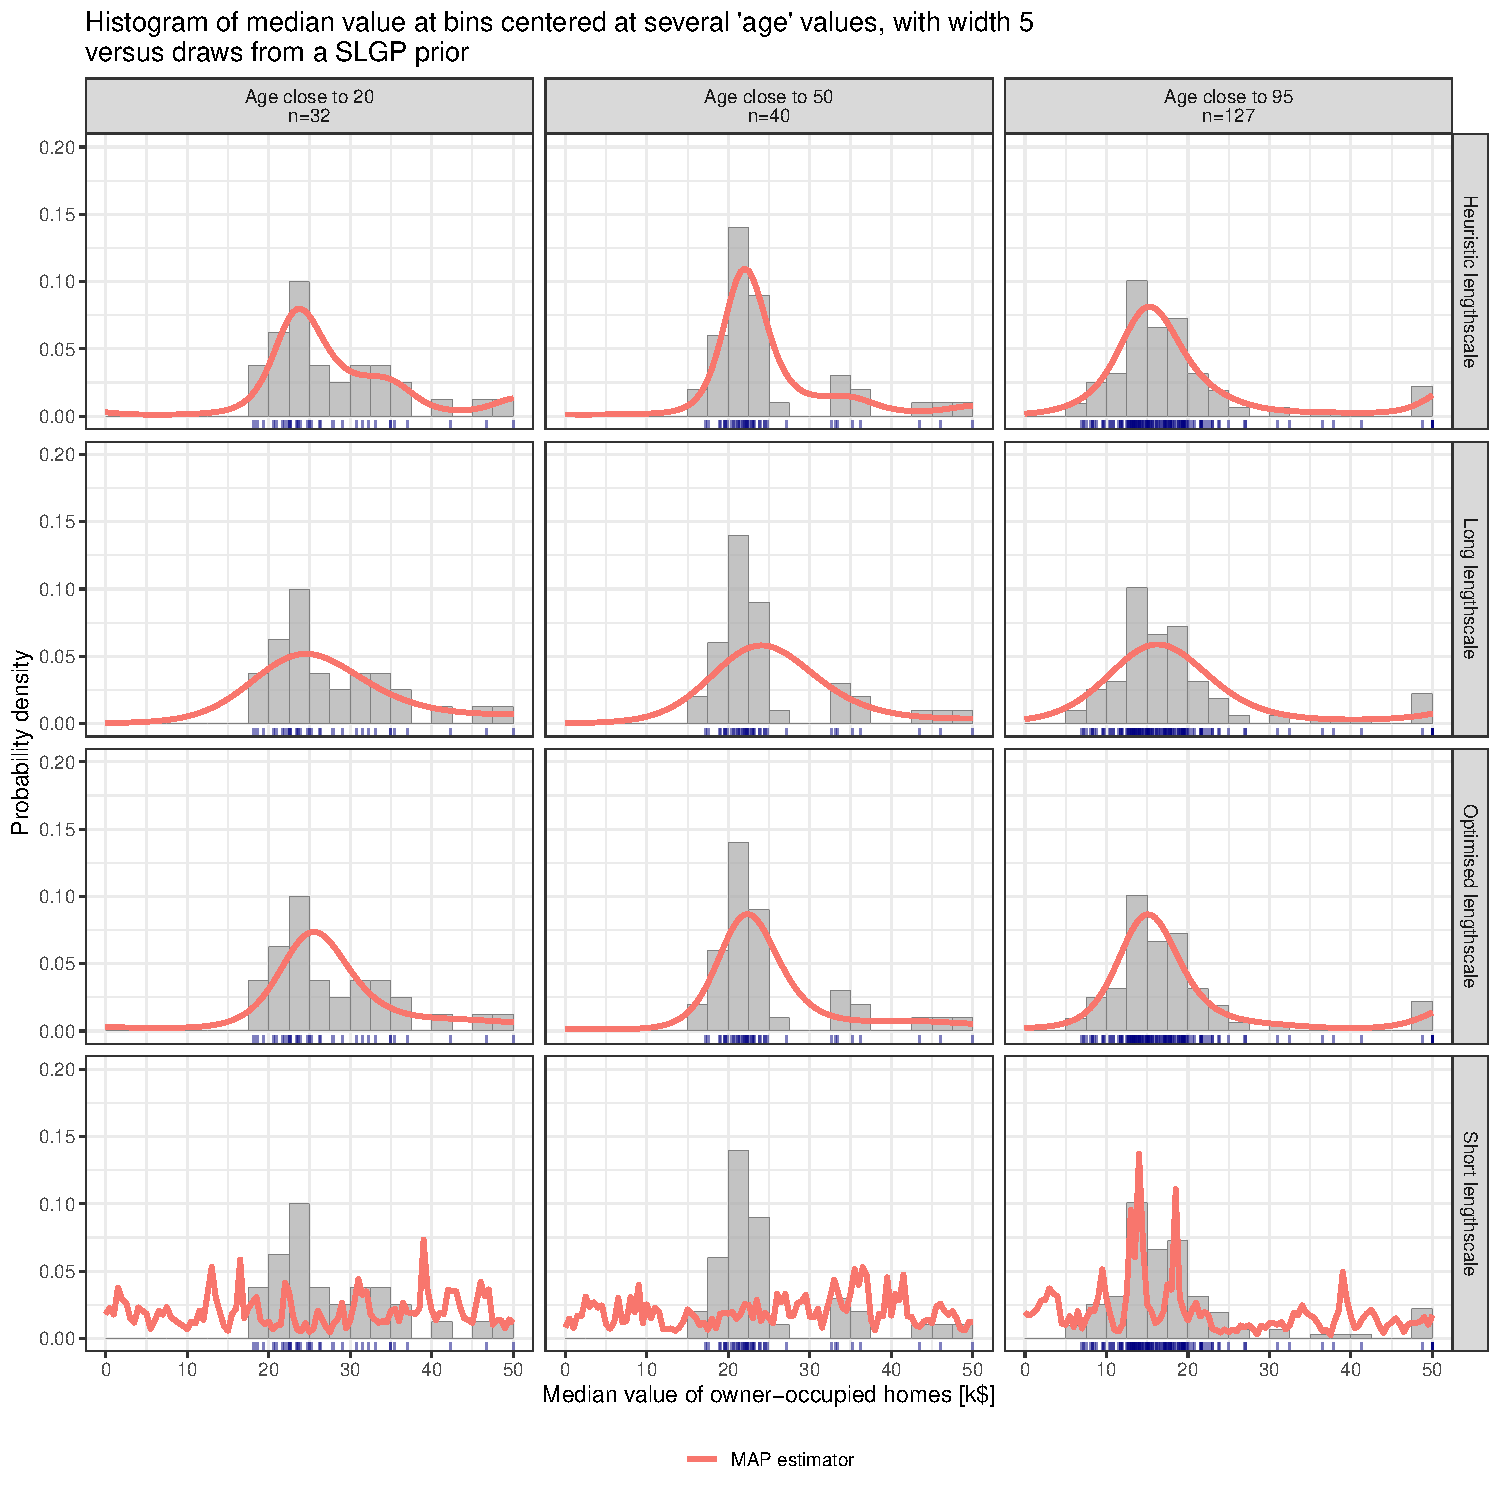
\includegraphics{IntroductionSLGP_files/figure-latex/plotRibbonsLen2-1} 

}

\caption{Comparison of fitted densities under different lengthscale settings}\label{fig:plotRibbonsLen2}
\end{figure}

We observe that when the lengthscale is too big, while the model captures the general support of the distribution, it fails to capture finer details, such as multi-modalities in certain distributions. This limitation likely arises from using a large lengthscale, which oversmooths small-scale variations.
On the opposite using too small a length scale restricts the model's spatial aggregation, limiting the reach of spatial information to a very local scope.

Using a heuristic as before, or the optimised version yield a compromise between the previously observed limitations.
For simplicity, we will continue with the lengthscales yielded by the heuristic, set to 15\% of the ranges.

\subsection{Laplace approximation estimate}\label{laplace-approximation-estimate}

By integrating the MAP approach with Laplace approximation, we refine our estimation strategy by approximating the posterior distribution with a multivariate Gaussian. This method strikes a balance between the full Bayesian inference of MCMC and the computational efficiency of MAP estimation. By leveraging both the gradient and Hessian of the posterior, it captures essential curvature information, providing a more informed approximation of the posterior landscape.

As for MAP, we could have use all three implementations: training from scratch, re-training a model or manually specifying components. We go for the second.

\begin{Shaded}
\begin{Highlighting}[]
\CommentTok{\# Or equivalent, re{-}use the same basis functions }
\CommentTok{\# and hyper parameters as in the prior we saw}

\NormalTok{modelLaplace }\OtherTok{\textless{}{-}} \FunctionTok{retrainSLGP}\NormalTok{(}\AttributeTok{SLGPmodel=}\NormalTok{modelPrior, }
                            \AttributeTok{newdata =}\NormalTok{ df, }
                            \AttributeTok{method=}\StringTok{"Laplace"}\NormalTok{)}
\end{Highlighting}
\end{Shaded}

Unlike MAP estimation, which provides only a point estimate, the Laplace approximation allows us to visualize uncertainty. To highlight this aspect, we compare multiple posterior draws from the approximation against histogram data, emphasizing how the estimated conditional density fluctuates. The figure below illustrates this by overlaying samples from the posterior approximation with binned data, showcasing the range of possible densities rather than focusing solely on the MAP estimate.

\begin{Shaded}
\begin{Highlighting}[]
\CommentTok{\# Define the three selected values}
\NormalTok{selected\_values }\OtherTok{\textless{}{-}} \FunctionTok{c}\NormalTok{(}\DecValTok{20}\NormalTok{, }\DecValTok{50}\NormalTok{, }\DecValTok{95}\NormalTok{)}
\NormalTok{gap }\OtherTok{\textless{}{-}} \DecValTok{5}

\NormalTok{dfGrid }\OtherTok{\textless{}{-}} \FunctionTok{data.frame}\NormalTok{(}\FunctionTok{expand.grid}\NormalTok{(}\FunctionTok{seq}\NormalTok{(}\DecValTok{3}\NormalTok{), }
                                 \FunctionTok{seq}\NormalTok{(range\_response[}\DecValTok{1}\NormalTok{], range\_response[}\DecValTok{2}\NormalTok{],, }\DecValTok{101}\NormalTok{)))}
\FunctionTok{colnames}\NormalTok{(dfGrid) }\OtherTok{\textless{}{-}} \FunctionTok{c}\NormalTok{(}\StringTok{"ID"}\NormalTok{, }\StringTok{"medv"}\NormalTok{)}
\NormalTok{dfGrid}\SpecialCharTok{$}\NormalTok{age }\OtherTok{\textless{}{-}}\NormalTok{ selected\_values[dfGrid}\SpecialCharTok{$}\NormalTok{ID]}
\NormalTok{pred }\OtherTok{\textless{}{-}} \FunctionTok{predictSLGP\_newNode}\NormalTok{(}\AttributeTok{SLGPmodel=}\NormalTok{modelLaplace,}
                            \AttributeTok{newNodes =}\NormalTok{ dfGrid)}
\NormalTok{pred}\SpecialCharTok{$}\NormalTok{meanpdf }\OtherTok{\textless{}{-}} \FunctionTok{rowMeans}\NormalTok{(pred[, }\SpecialCharTok{{-}}\FunctionTok{c}\NormalTok{(}\DecValTok{1}\SpecialCharTok{:}\DecValTok{3}\NormalTok{)])}

\FunctionTok{library}\NormalTok{(tidyr)}
\CommentTok{\# Filter the data: keep values within ±5 of the selected ones}
\NormalTok{df\_filtered }\OtherTok{\textless{}{-}}\NormalTok{ df }\SpecialCharTok{\%\textgreater{}\%}
  \FunctionTok{mutate}\NormalTok{(}\AttributeTok{interval=}\FunctionTok{findInterval}\NormalTok{(age, }\FunctionTok{c}\NormalTok{(}\DecValTok{0}\NormalTok{, }
\NormalTok{                                      selected\_values[}\DecValTok{1}\NormalTok{]}\SpecialCharTok{{-}}\NormalTok{gap, }
\NormalTok{                                      selected\_values[}\DecValTok{1}\NormalTok{]}\SpecialCharTok{+}\NormalTok{gap, }
\NormalTok{                                      selected\_values[}\DecValTok{2}\NormalTok{]}\SpecialCharTok{{-}}\NormalTok{gap, }
\NormalTok{                                      selected\_values[}\DecValTok{2}\NormalTok{]}\SpecialCharTok{+}\NormalTok{gap, }
\NormalTok{                                      selected\_values[}\DecValTok{3}\NormalTok{]}\SpecialCharTok{{-}}\NormalTok{gap, }
\NormalTok{                                      selected\_values[}\DecValTok{3}\NormalTok{]}\SpecialCharTok{+}\NormalTok{gap)))}\SpecialCharTok{\%\textgreater{}\%}
  \FunctionTok{filter}\NormalTok{(interval }\SpecialCharTok{\%in\%} \FunctionTok{c}\NormalTok{(}\DecValTok{2}\NormalTok{, }\DecValTok{4}\NormalTok{, }\DecValTok{6}\NormalTok{))}\SpecialCharTok{\%\textgreater{}\%}
  \FunctionTok{group\_by}\NormalTok{(interval)}\SpecialCharTok{\%\textgreater{}\%}
  \FunctionTok{mutate}\NormalTok{(}\AttributeTok{category =} \FunctionTok{paste0}\NormalTok{(}\StringTok{"Age close to "}\NormalTok{, }\FunctionTok{c}\NormalTok{(}\StringTok{""}\NormalTok{, selected\_values[}\DecValTok{1}\NormalTok{],}
                                              \StringTok{""}\NormalTok{, selected\_values[}\DecValTok{2}\NormalTok{],}
                                              \StringTok{""}\NormalTok{, selected\_values[}\DecValTok{3}\NormalTok{])[interval], }
                           \StringTok{"}\SpecialCharTok{\textbackslash{}n}\StringTok{n="}\NormalTok{, }\FunctionTok{n}\NormalTok{()))}
\NormalTok{names }\OtherTok{\textless{}{-}} \FunctionTok{sort}\NormalTok{(}\FunctionTok{unique}\NormalTok{(df\_filtered}\SpecialCharTok{$}\NormalTok{category))}
\NormalTok{pred}\SpecialCharTok{$}\NormalTok{category }\OtherTok{\textless{}{-}}\NormalTok{ names[pred}\SpecialCharTok{$}\NormalTok{ID]}

\FunctionTok{set.seed}\NormalTok{(}\DecValTok{1}\NormalTok{)}
\NormalTok{selected\_cols }\OtherTok{\textless{}{-}} \FunctionTok{sample}\NormalTok{(}\FunctionTok{seq}\NormalTok{(}\DecValTok{1000}\NormalTok{), }\AttributeTok{size=}\DecValTok{10}\NormalTok{, }\AttributeTok{replace=}\ConstantTok{FALSE}\NormalTok{)}
\NormalTok{df\_plot }\OtherTok{\textless{}{-}}\NormalTok{ pred }\SpecialCharTok{\%\textgreater{}\%}
\NormalTok{  dplyr}\SpecialCharTok{::}\FunctionTok{select}\NormalTok{(}\FunctionTok{c}\NormalTok{(}\StringTok{"age"}\NormalTok{, }\StringTok{"medv"}\NormalTok{, }\StringTok{"category"}\NormalTok{, }
                  \FunctionTok{paste0}\NormalTok{(}\StringTok{"pdf\_"}\NormalTok{, selected\_cols)))}\SpecialCharTok{\%\textgreater{}\%}
  \FunctionTok{pivot\_longer}\NormalTok{(}\SpecialCharTok{{-}}\FunctionTok{c}\NormalTok{(}\StringTok{"age"}\NormalTok{, }\StringTok{"medv"}\NormalTok{, }\StringTok{"category"}\NormalTok{))}


\FunctionTok{ggplot}\NormalTok{(}\AttributeTok{mapping=}\FunctionTok{aes}\NormalTok{(}\AttributeTok{x =}\NormalTok{ medv)) }\SpecialCharTok{+}
  \FunctionTok{geom\_histogram}\NormalTok{(df\_filtered,}
                 \AttributeTok{mapping=}\FunctionTok{aes}\NormalTok{(}\AttributeTok{y=}\FunctionTok{after\_stat}\NormalTok{(density)),}
                 \AttributeTok{position =} \StringTok{"identity"}\NormalTok{, }\AttributeTok{breaks =} \FunctionTok{seq}\NormalTok{(}\DecValTok{0}\NormalTok{, }\DecValTok{50}\NormalTok{, }\FloatTok{2.5}\NormalTok{),}
                 \AttributeTok{fill=}\StringTok{"darkgrey"}\NormalTok{, }\AttributeTok{col=}\StringTok{"grey50"}\NormalTok{, }\AttributeTok{lwd=}\FloatTok{0.2}\NormalTok{, }\AttributeTok{alpha=}\FloatTok{0.7}\NormalTok{) }\SpecialCharTok{+}
  \FunctionTok{geom\_rug}\NormalTok{(}\AttributeTok{data=}\NormalTok{df\_filtered, }\AttributeTok{sides =} \StringTok{"b"}\NormalTok{, }\AttributeTok{color =} \StringTok{"navy"}\NormalTok{, }\AttributeTok{alpha =} \FloatTok{0.5}\NormalTok{)}\SpecialCharTok{+}
  \FunctionTok{geom\_line}\NormalTok{(}\AttributeTok{data=}\NormalTok{df\_plot, }\AttributeTok{mapping=}\FunctionTok{aes}\NormalTok{(}\AttributeTok{y=}\NormalTok{value, }\AttributeTok{group=}\NormalTok{name), }
            \AttributeTok{color =} \StringTok{"black"}\NormalTok{, }\AttributeTok{lwd=}\FloatTok{0.1}\NormalTok{, }\AttributeTok{alpha=}\FloatTok{0.5}\NormalTok{)}\SpecialCharTok{+}
  \FunctionTok{geom\_line}\NormalTok{(}\AttributeTok{data=}\NormalTok{pred, }\AttributeTok{mapping=}\FunctionTok{aes}\NormalTok{(}\AttributeTok{y=}\NormalTok{meanpdf, }\AttributeTok{group=}\NormalTok{category), }\AttributeTok{color =} \StringTok{"red"}\NormalTok{)}\SpecialCharTok{+}
  \FunctionTok{facet\_wrap}\NormalTok{(}\SpecialCharTok{\textasciitilde{}}\NormalTok{ category, }\AttributeTok{scales =} \StringTok{"free\_y"}\NormalTok{, }\AttributeTok{nrow=}\DecValTok{1}\NormalTok{) }\SpecialCharTok{+}
  \FunctionTok{labs}\NormalTok{(}\AttributeTok{x =} \StringTok{"Median value of owner{-}occupied homes [k$]"}\NormalTok{, }
       \AttributeTok{y =} \StringTok{"Probability density"}\NormalTok{, }
       \AttributeTok{title =} \StringTok{"Histogram of median value at bins centered at several \textquotesingle{}age\textquotesingle{} values, with width 5}\SpecialCharTok{\textbackslash{}n}\StringTok{versus SLGP draws from a laplace approximation (black curves) and average (red curve)"}\NormalTok{) }\SpecialCharTok{+}
  \FunctionTok{theme\_bw}\NormalTok{()}\SpecialCharTok{+}
  \FunctionTok{coord\_cartesian}\NormalTok{(}\AttributeTok{xlim=}\NormalTok{range\_response,}
                  \AttributeTok{ylim=}\FunctionTok{c}\NormalTok{(}\DecValTok{0}\NormalTok{, }\FloatTok{0.25}\NormalTok{))}
\end{Highlighting}
\end{Shaded}

\begin{figure}[H]

{\centering 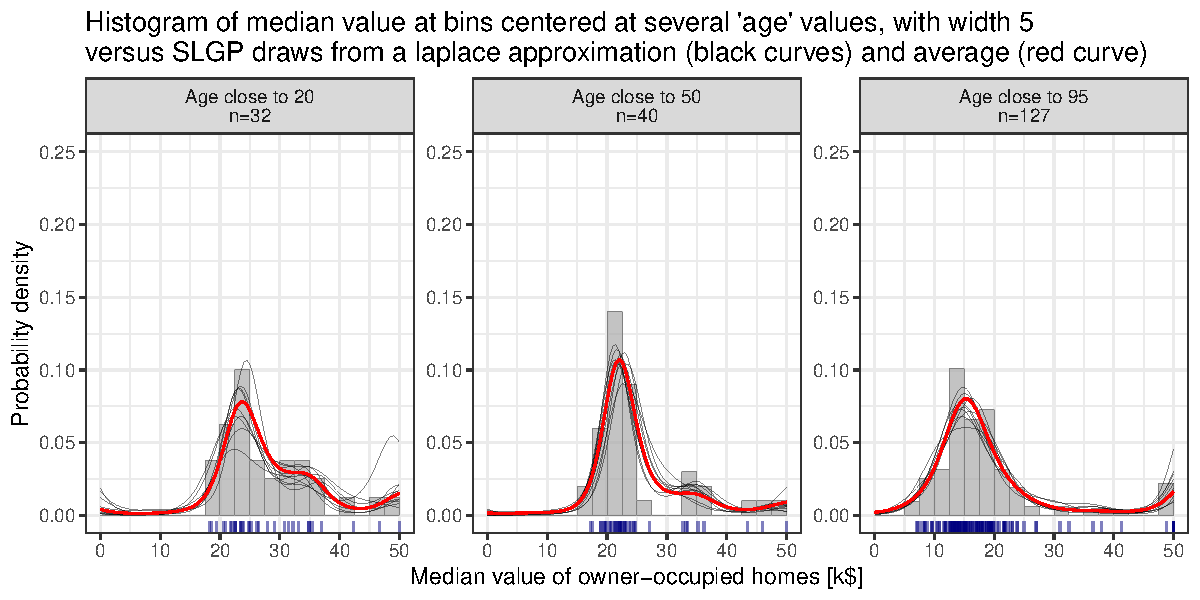
\includegraphics{IntroductionSLGP_files/figure-latex/SLGPLaplaceplot-1} 

}

\caption{Predictive probability density (and draws from a Laplace approximation) of medv at age, seen over 3 slices.}\label{fig:SLGPLaplaceplot}
\end{figure}

\subsection{MCMC estimate}\label{mcmc-estimate}

This method allows us to fully explore the posterior distribution by drawing samples from it. Unlike MAP or Laplace approximation, which provide a single point estimate or a Gaussian approximation, MCMC enables exact Bayesian inference of the underlying density field, given the observed data. The main drawback of this approach being its higher computational cost

As for MAP and Laplace, we could have used all three implementations: training from scratch, re-training a model or manually specifying components. We go for the second again.

\begin{Shaded}
\begin{Highlighting}[]
\ControlFlowTok{if}\NormalTok{(}\SpecialCharTok{!}\FunctionTok{file.exists}\NormalTok{(}\StringTok{"modelMCMC.Rdata"}\NormalTok{))\{}
\NormalTok{  modelMCMC  }\OtherTok{\textless{}{-}} \FunctionTok{retrainSLGP}\NormalTok{(}\AttributeTok{SLGPmodel=}\NormalTok{modelPrior, }
                            \AttributeTok{newdata =}\NormalTok{ df, }
                            \AttributeTok{method=}\StringTok{"MCMC"}\NormalTok{,}
                            \AttributeTok{opts =} \FunctionTok{list}\NormalTok{(}\AttributeTok{stan\_chains=}\DecValTok{2}\NormalTok{, }\AttributeTok{stan\_iter=}\DecValTok{1000}\NormalTok{))}
  \FunctionTok{save}\NormalTok{(modelMCMC, }\AttributeTok{file=}\StringTok{"modelMCMC.Rdata"}\NormalTok{)}
  
\NormalTok{\}}\ControlFlowTok{else}\NormalTok{\{}
  \FunctionTok{load}\NormalTok{(}\StringTok{"modelMCMC.Rdata"}\NormalTok{)}
\NormalTok{\}}
\end{Highlighting}
\end{Shaded}

MCMC provides a rich representation of uncertainty in the estimated density. Instead of showing a single estimate, we compare multiple posterior draws against histogram data, similarly to what we did for the Laplace approximation.

\begin{Shaded}
\begin{Highlighting}[]
\CommentTok{\# Define the three selected values}
\NormalTok{pred }\OtherTok{\textless{}{-}} \FunctionTok{predictSLGP\_newNode}\NormalTok{(}\AttributeTok{SLGPmodel=}\NormalTok{modelMCMC,}
                            \AttributeTok{newNodes =}\NormalTok{ dfGrid)}
\NormalTok{pred}\SpecialCharTok{$}\NormalTok{meanpdf }\OtherTok{\textless{}{-}} \FunctionTok{rowMeans}\NormalTok{(pred[, }\SpecialCharTok{{-}}\FunctionTok{c}\NormalTok{(}\DecValTok{1}\SpecialCharTok{:}\DecValTok{3}\NormalTok{)])}
\NormalTok{pred}\SpecialCharTok{$}\NormalTok{category }\OtherTok{\textless{}{-}}\NormalTok{ names[pred}\SpecialCharTok{$}\NormalTok{ID]}

\NormalTok{df\_plot }\OtherTok{\textless{}{-}}\NormalTok{ pred }\SpecialCharTok{\%\textgreater{}\%}
\NormalTok{  dplyr}\SpecialCharTok{::}\FunctionTok{select}\NormalTok{(}\FunctionTok{c}\NormalTok{(}\StringTok{"age"}\NormalTok{, }\StringTok{"medv"}\NormalTok{, }\StringTok{"category"}\NormalTok{, }
                  \FunctionTok{paste0}\NormalTok{(}\StringTok{"pdf\_"}\NormalTok{, selected\_cols)))}\SpecialCharTok{\%\textgreater{}\%}
  \FunctionTok{pivot\_longer}\NormalTok{(}\SpecialCharTok{{-}}\FunctionTok{c}\NormalTok{(}\StringTok{"age"}\NormalTok{, }\StringTok{"medv"}\NormalTok{, }\StringTok{"category"}\NormalTok{))}


\FunctionTok{ggplot}\NormalTok{(}\AttributeTok{mapping=}\FunctionTok{aes}\NormalTok{(}\AttributeTok{x =}\NormalTok{ medv)) }\SpecialCharTok{+}
  \FunctionTok{geom\_histogram}\NormalTok{(df\_filtered,}
                 \AttributeTok{mapping=}\FunctionTok{aes}\NormalTok{(}\AttributeTok{y=}\FunctionTok{after\_stat}\NormalTok{(density)),}
                 \AttributeTok{position =} \StringTok{"identity"}\NormalTok{, }\AttributeTok{breaks =} \FunctionTok{seq}\NormalTok{(}\DecValTok{0}\NormalTok{, }\DecValTok{50}\NormalTok{, }\FloatTok{2.5}\NormalTok{),}
                 \AttributeTok{fill=}\StringTok{"darkgrey"}\NormalTok{, }\AttributeTok{col=}\StringTok{"grey50"}\NormalTok{, }\AttributeTok{lwd=}\FloatTok{0.2}\NormalTok{, }\AttributeTok{alpha=}\FloatTok{0.7}\NormalTok{) }\SpecialCharTok{+}
  \FunctionTok{geom\_rug}\NormalTok{(}\AttributeTok{data=}\NormalTok{df\_filtered, }\AttributeTok{sides =} \StringTok{"b"}\NormalTok{, }\AttributeTok{color =} \StringTok{"navy"}\NormalTok{, }\AttributeTok{alpha =} \FloatTok{0.5}\NormalTok{)}\SpecialCharTok{+}
  \FunctionTok{geom\_line}\NormalTok{(}\AttributeTok{data=}\NormalTok{df\_plot, }\AttributeTok{mapping=}\FunctionTok{aes}\NormalTok{(}\AttributeTok{y=}\NormalTok{value, }\AttributeTok{group=}\NormalTok{name), }
            \AttributeTok{color =} \StringTok{"black"}\NormalTok{, }\AttributeTok{lwd=}\FloatTok{0.1}\NormalTok{, }\AttributeTok{alpha=}\FloatTok{0.5}\NormalTok{)}\SpecialCharTok{+}
  \FunctionTok{geom\_line}\NormalTok{(}\AttributeTok{data=}\NormalTok{pred, }\AttributeTok{mapping=}\FunctionTok{aes}\NormalTok{(}\AttributeTok{y=}\NormalTok{meanpdf, }\AttributeTok{group=}\NormalTok{category), }\AttributeTok{color =} \StringTok{"red"}\NormalTok{)}\SpecialCharTok{+}
  \FunctionTok{facet\_wrap}\NormalTok{(}\SpecialCharTok{\textasciitilde{}}\NormalTok{ category, }\AttributeTok{scales =} \StringTok{"free\_y"}\NormalTok{, }\AttributeTok{nrow=}\DecValTok{1}\NormalTok{) }\SpecialCharTok{+}
  \FunctionTok{labs}\NormalTok{(}\AttributeTok{x =} \StringTok{"Median value of owner{-}occupied homes [k$]"}\NormalTok{, }
       \AttributeTok{y =} \StringTok{"Probability density"}\NormalTok{, }
       \AttributeTok{title =} \StringTok{"Histogram of median value at bins centered at several \textquotesingle{}age\textquotesingle{} values, with width 5}\SpecialCharTok{\textbackslash{}n}\StringTok{versus SLGP draws from a MCMC (black curves) and average (red curve)"}\NormalTok{) }\SpecialCharTok{+}
  \FunctionTok{theme\_bw}\NormalTok{()}\SpecialCharTok{+}
  \FunctionTok{coord\_cartesian}\NormalTok{(}\AttributeTok{xlim=}\NormalTok{range\_response,}
                  \AttributeTok{ylim=}\FunctionTok{c}\NormalTok{(}\DecValTok{0}\NormalTok{, }\FloatTok{0.25}\NormalTok{))}
\end{Highlighting}
\end{Shaded}

\begin{figure}[H]

{\centering 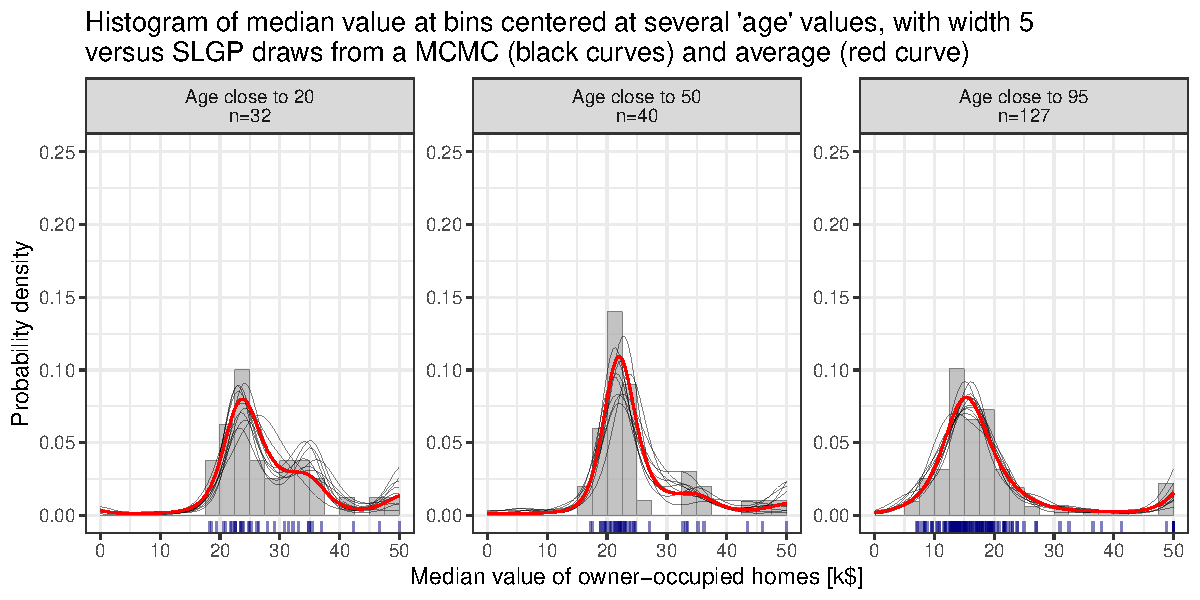
\includegraphics{IntroductionSLGP_files/figure-latex/SLGPMCMCplot-1} 

}

\caption{Predictive probability density (and draws from a MCMC) of medv at age, seen over 3 slices.}\label{fig:SLGPMCMCplot}
\end{figure}

\section{By-products of the estimation}\label{by-products-of-the-estimation}

One of the advantages of the SLGP framework is that it predicts entire probability density functions (PDFs) over space. This opens the door to a wide range of nonlinear inferences on the estimated field. In particular, we can compute and visualize functionals of the predicted densities, such as moments (mean, variance, skewness, etc.) or quantiles.

In our current implementation, we provide predictions for both centered and uncentered moments of the estimated PDFs at each location. These derived quantities can themselves be interpreted as spatial fields and are thus informative summaries of the underlying random process.

Importantly, when using probabilistic inference schemes like Laplace approximation or MCMC, the uncertainty in the SLGP predictions naturally propagates to these functionals. As a result, we can also quantify uncertainty on the functionals. For example, we compute credible intervals for the mean or variance field. This is illustrated in the upcoming figure, where we use the MCMC-trained SLGP model to compute moments.

\begin{Shaded}
\begin{Highlighting}[]
\NormalTok{dfX }\OtherTok{\textless{}{-}} \FunctionTok{data.frame}\NormalTok{(}\AttributeTok{age=}\FunctionTok{seq}\NormalTok{(range\_x[}\DecValTok{1}\NormalTok{], range\_x[}\DecValTok{2}\NormalTok{], }\DecValTok{1}\NormalTok{))}

\NormalTok{predMean }\OtherTok{\textless{}{-}} \FunctionTok{predictSLGP\_moments}\NormalTok{(}\AttributeTok{SLGPmodel=}\NormalTok{modelMCMC,}
                                \AttributeTok{newNodes =}\NormalTok{ dfX, }
                                \AttributeTok{power=}\FunctionTok{c}\NormalTok{(}\DecValTok{1}\NormalTok{),}
                                \AttributeTok{centered=}\ConstantTok{FALSE}\NormalTok{)}
\NormalTok{predVar }\OtherTok{\textless{}{-}} \FunctionTok{predictSLGP\_moments}\NormalTok{(}\AttributeTok{SLGPmodel=}\NormalTok{modelMCMC,}
                               \AttributeTok{newNodes =}\NormalTok{ dfX, }
                               \AttributeTok{power=}\FunctionTok{c}\NormalTok{(}\DecValTok{2}\NormalTok{, }\DecValTok{3}\NormalTok{, }\DecValTok{4}\NormalTok{), }
                               \AttributeTok{centered=}\ConstantTok{TRUE}\NormalTok{)}
\NormalTok{pred }\OtherTok{\textless{}{-}} \FunctionTok{rbind}\NormalTok{(predMean, predVar)}
\NormalTok{pred }\OtherTok{\textless{}{-}}\NormalTok{ pred }\SpecialCharTok{\%\textgreater{}\%}
  \FunctionTok{pivot\_longer}\NormalTok{(}\SpecialCharTok{{-}}\FunctionTok{c}\NormalTok{(}\StringTok{"age"}\NormalTok{, }\StringTok{"power"}\NormalTok{))}\SpecialCharTok{\%\textgreater{}\%}
  \FunctionTok{mutate}\NormalTok{(}\AttributeTok{value=}\FunctionTok{ifelse}\NormalTok{(power}\SpecialCharTok{==}\DecValTok{2}\NormalTok{, }\FunctionTok{sqrt}\NormalTok{(value), value))}\SpecialCharTok{\%\textgreater{}\%}
  \FunctionTok{pivot\_wider}\NormalTok{(}\AttributeTok{values\_from =}\NormalTok{ value,}
              \AttributeTok{names\_from =}\NormalTok{ power)}\SpecialCharTok{\%\textgreater{}\%}
  \FunctionTok{mutate}\NormalTok{(}\StringTok{\textasciigrave{}}\AttributeTok{3}\StringTok{\textasciigrave{}}\OtherTok{=}\StringTok{\textasciigrave{}}\AttributeTok{3}\StringTok{\textasciigrave{}}\SpecialCharTok{/}\StringTok{\textasciigrave{}}\AttributeTok{2}\StringTok{\textasciigrave{}}\SpecialCharTok{\^{}}\DecValTok{2}\NormalTok{,}
         \StringTok{\textasciigrave{}}\AttributeTok{4}\StringTok{\textasciigrave{}}\OtherTok{=}\StringTok{\textasciigrave{}}\AttributeTok{4}\StringTok{\textasciigrave{}}\SpecialCharTok{/}\StringTok{\textasciigrave{}}\AttributeTok{2}\StringTok{\textasciigrave{}}\SpecialCharTok{\^{}}\DecValTok{4}\NormalTok{)}\SpecialCharTok{\%\textgreater{}\%}
  \FunctionTok{pivot\_longer}\NormalTok{(}\SpecialCharTok{{-}}\FunctionTok{c}\NormalTok{(}\StringTok{"age"}\NormalTok{, }\StringTok{"name"}\NormalTok{), }\AttributeTok{names\_to =} \StringTok{"power"}\NormalTok{)}\SpecialCharTok{\%\textgreater{}\%}
  \FunctionTok{data.frame}\NormalTok{()}
\CommentTok{\#\textgreater{} Warning: There was 1 warning in \textasciigrave{}mutate()\textasciigrave{}.}
\CommentTok{\#\textgreater{} i In argument: \textasciigrave{}value = ifelse(power == 2, sqrt(value), value)\textasciigrave{}.}
\CommentTok{\#\textgreater{} Caused by warning in \textasciigrave{}sqrt()\textasciigrave{}:}
\CommentTok{\#\textgreater{} ! Production de NaN}

\NormalTok{pred}\SpecialCharTok{$}\NormalTok{power }\OtherTok{\textless{}{-}} \FunctionTok{factor}\NormalTok{(}\FunctionTok{c}\NormalTok{(}\StringTok{"Expected value"}\NormalTok{, }
                       \StringTok{"Standard deviation"}\NormalTok{,}
                       \StringTok{"Skewness"}\NormalTok{,}\StringTok{"Kurtosis"}\NormalTok{)[}\FunctionTok{as.numeric}\NormalTok{(pred}\SpecialCharTok{$}\NormalTok{power)],}
                     \AttributeTok{levels=}\FunctionTok{c}\NormalTok{(}\StringTok{"Expected value"}\NormalTok{, }\StringTok{"Standard deviation"}\NormalTok{,}
                              \StringTok{"Skewness"}\NormalTok{, }\StringTok{"Kurtosis"}\NormalTok{))}
\NormalTok{df\_plot }\OtherTok{\textless{}{-}}\NormalTok{ pred }\SpecialCharTok{\%\textgreater{}\%}
  \FunctionTok{group\_by}\NormalTok{(age, power)}\SpecialCharTok{\%\textgreater{}\%}
  \FunctionTok{summarise}\NormalTok{(}\AttributeTok{q10 =} \FunctionTok{quantile}\NormalTok{(value, }\AttributeTok{probs=}\FunctionTok{c}\NormalTok{(}\FloatTok{0.1}\NormalTok{)),}
            \AttributeTok{q50 =} \FunctionTok{quantile}\NormalTok{(value, }\AttributeTok{probs=}\FunctionTok{c}\NormalTok{(}\FloatTok{0.5}\NormalTok{)),}
            \AttributeTok{q90 =} \FunctionTok{quantile}\NormalTok{(value, }\AttributeTok{probs=}\FunctionTok{c}\NormalTok{(}\FloatTok{0.9}\NormalTok{)),}
            \AttributeTok{mean =} \FunctionTok{mean}\NormalTok{(value), }\AttributeTok{.groups=}\StringTok{"keep"}\NormalTok{)}\SpecialCharTok{\%\textgreater{}\%}
  \FunctionTok{ungroup}\NormalTok{()}


\FunctionTok{ggplot}\NormalTok{(df\_plot, }\AttributeTok{mapping=}\FunctionTok{aes}\NormalTok{(}\AttributeTok{x =}\NormalTok{ age)) }\SpecialCharTok{+}
  \FunctionTok{geom\_ribbon}\NormalTok{(}\AttributeTok{mapping =} \FunctionTok{aes}\NormalTok{(}\AttributeTok{ymin=}\NormalTok{q10, }\AttributeTok{ymax=}\NormalTok{q90),}
              \AttributeTok{alpha =} \FloatTok{0.25}\NormalTok{, }\AttributeTok{lty=}\DecValTok{2}\NormalTok{, }\AttributeTok{col=}\StringTok{"black"}\NormalTok{, }\AttributeTok{fill=}\StringTok{"cornflowerblue"}\NormalTok{)}\SpecialCharTok{+}
  \FunctionTok{geom\_line}\NormalTok{(}\AttributeTok{mapping=}\FunctionTok{aes}\NormalTok{(}\AttributeTok{y=}\NormalTok{q50))}\SpecialCharTok{+}
  \FunctionTok{facet\_grid}\NormalTok{(.}\SpecialCharTok{\textasciitilde{}}\NormalTok{power)}\SpecialCharTok{+}
  \FunctionTok{labs}\NormalTok{(}\AttributeTok{x =} \StringTok{"Proportion of owner{-}occupied units}\SpecialCharTok{\textbackslash{}n}\StringTok{built prior to 1940 [AGE, \%]"}\NormalTok{, }
       \AttributeTok{y =} \StringTok{"Median value of owner{-}occupied homes [MEDV, k$]"}\NormalTok{) }\SpecialCharTok{+}
  \FunctionTok{theme\_bw}\NormalTok{()}\SpecialCharTok{+}
  \FunctionTok{coord\_cartesian}\NormalTok{(}\AttributeTok{xlim=}\NormalTok{range\_x,}
                  \AttributeTok{ylim=}\NormalTok{range\_response)}
\end{Highlighting}
\end{Shaded}

\begin{figure}[H]

{\centering 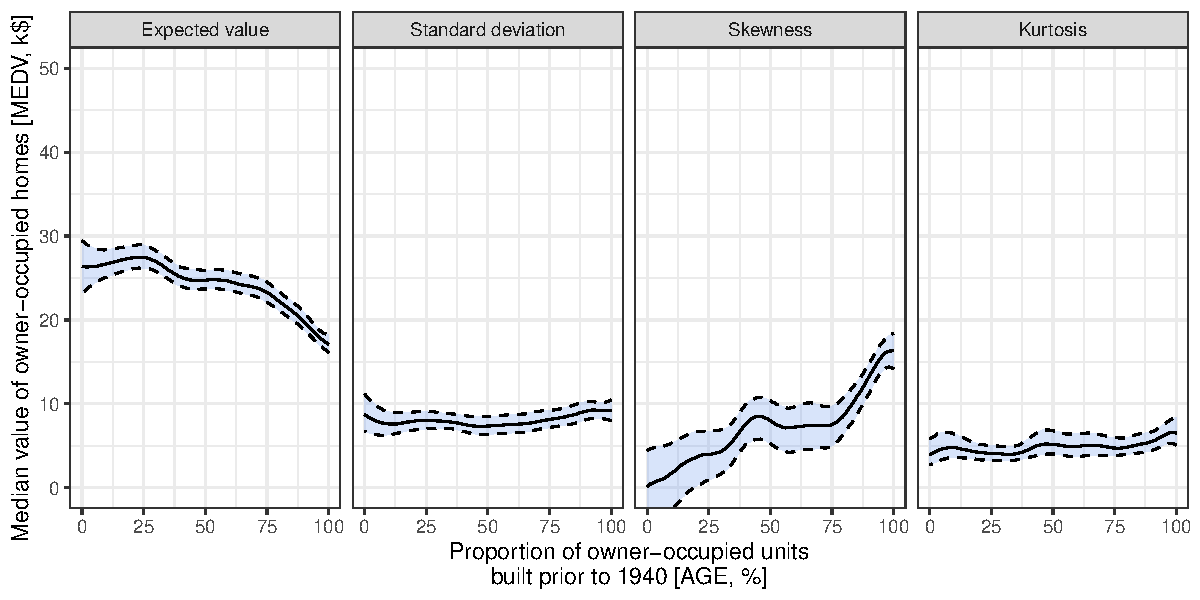
\includegraphics{IntroductionSLGP_files/figure-latex/SLGPMCMCplotMoments-1} 

}

\caption{Simultaneous prediction of the fields moments (and associated uncertainty) using a SLGP model}\label{fig:SLGPMCMCplotMoments}
\end{figure}

We also support the joint prediction of quantiles at arbitrary levels. Because quantiles are derived directly from the estimated densities, they are guaranteed to be consistent and non-crossing - a property that cannot always be ensured in standard quantile regression. This makes them reliable tools for summarizing distributional shape (e.g., asymmetry, spread) at each location.

\begin{Shaded}
\begin{Highlighting}[]
\CommentTok{\# Define the three selected values}

\NormalTok{probsL }\OtherTok{\textless{}{-}} \FunctionTok{c}\NormalTok{(}\DecValTok{5}\NormalTok{, }\DecValTok{25}\NormalTok{, }\DecValTok{50}\NormalTok{, }\DecValTok{75}\NormalTok{, }\DecValTok{95}\NormalTok{)}\SpecialCharTok{/}\DecValTok{100}

\NormalTok{pred }\OtherTok{\textless{}{-}} \FunctionTok{predictSLGP\_quantiles}\NormalTok{(}\AttributeTok{SLGPmodel=}\NormalTok{modelMCMC,}
                              \AttributeTok{newNodes =}\NormalTok{ dfX, }
                              \AttributeTok{probs=}\NormalTok{probsL)}


\NormalTok{df\_plot }\OtherTok{\textless{}{-}}\NormalTok{ pred }\SpecialCharTok{\%\textgreater{}\%}
  \FunctionTok{pivot\_longer}\NormalTok{(}\SpecialCharTok{{-}}\FunctionTok{c}\NormalTok{(}\StringTok{"age"}\NormalTok{, }\StringTok{"probs"}\NormalTok{))}\SpecialCharTok{\%\textgreater{}\%}
  \FunctionTok{group\_by}\NormalTok{(age, probs)}\SpecialCharTok{\%\textgreater{}\%}
  \FunctionTok{summarise}\NormalTok{(}\AttributeTok{q10 =} \FunctionTok{quantile}\NormalTok{(value, }\AttributeTok{probs=}\FunctionTok{c}\NormalTok{(}\FloatTok{0.1}\NormalTok{)),}
            \AttributeTok{q50 =} \FunctionTok{quantile}\NormalTok{(value, }\AttributeTok{probs=}\FunctionTok{c}\NormalTok{(}\FloatTok{0.5}\NormalTok{)),}
            \AttributeTok{q90 =} \FunctionTok{quantile}\NormalTok{(value, }\AttributeTok{probs=}\FunctionTok{c}\NormalTok{(}\FloatTok{0.9}\NormalTok{)),}
            \AttributeTok{mean =} \FunctionTok{mean}\NormalTok{(value), }\AttributeTok{.groups=}\StringTok{"keep"}\NormalTok{)}\SpecialCharTok{\%\textgreater{}\%}
  \FunctionTok{ungroup}\NormalTok{()}\SpecialCharTok{\%\textgreater{}\%}
  \FunctionTok{mutate}\NormalTok{(}\AttributeTok{probs=}\FunctionTok{factor}\NormalTok{(}\FunctionTok{paste0}\NormalTok{(}\StringTok{"Quantile: "}\NormalTok{, }\DecValTok{100}\SpecialCharTok{*}\NormalTok{probs, }\StringTok{"\%"}\NormalTok{),}
                      \AttributeTok{levels=}\FunctionTok{paste0}\NormalTok{(}\StringTok{"Quantile: "}\NormalTok{, }\DecValTok{100}\SpecialCharTok{*}\NormalTok{probsL, }\StringTok{"\%"}\NormalTok{)))}


\FunctionTok{ggplot}\NormalTok{(df\_plot, }\AttributeTok{mapping=}\FunctionTok{aes}\NormalTok{(}\AttributeTok{x =}\NormalTok{ age, }\AttributeTok{col=}\NormalTok{probs, }\AttributeTok{fill=}\NormalTok{probs, }\AttributeTok{group=}\NormalTok{probs)) }\SpecialCharTok{+}
  \FunctionTok{geom\_ribbon}\NormalTok{(}\AttributeTok{mapping =} \FunctionTok{aes}\NormalTok{(}\AttributeTok{ymin=}\NormalTok{q10, }\AttributeTok{ymax=}\NormalTok{q90),}
              \AttributeTok{alpha =} \FloatTok{0.25}\NormalTok{, }\AttributeTok{lty=}\DecValTok{2}\NormalTok{)}\SpecialCharTok{+}
  \FunctionTok{geom\_line}\NormalTok{(}\AttributeTok{mapping=}\FunctionTok{aes}\NormalTok{(}\AttributeTok{y=}\NormalTok{q50))}\SpecialCharTok{+}
  \FunctionTok{labs}\NormalTok{(}\AttributeTok{x =} \StringTok{"Proportion of owner{-}occupied units}\SpecialCharTok{\textbackslash{}n}\StringTok{built prior to 1940 [AGE, \%]"}\NormalTok{, }
       \AttributeTok{y =} \StringTok{"Median value of owner{-}occupied homes [MEDV, k$]"}\NormalTok{,}
       \AttributeTok{fill =} \StringTok{"Quantile levels"}\NormalTok{,}
       \AttributeTok{col =} \StringTok{"Quantile levels"}\NormalTok{) }\SpecialCharTok{+}
  \FunctionTok{theme\_bw}\NormalTok{()}\SpecialCharTok{+}
  \FunctionTok{coord\_cartesian}\NormalTok{(}\AttributeTok{xlim=}\NormalTok{range\_x,}
                  \AttributeTok{ylim=}\NormalTok{range\_response)}
\end{Highlighting}
\end{Shaded}

\begin{figure}[H]

{\centering 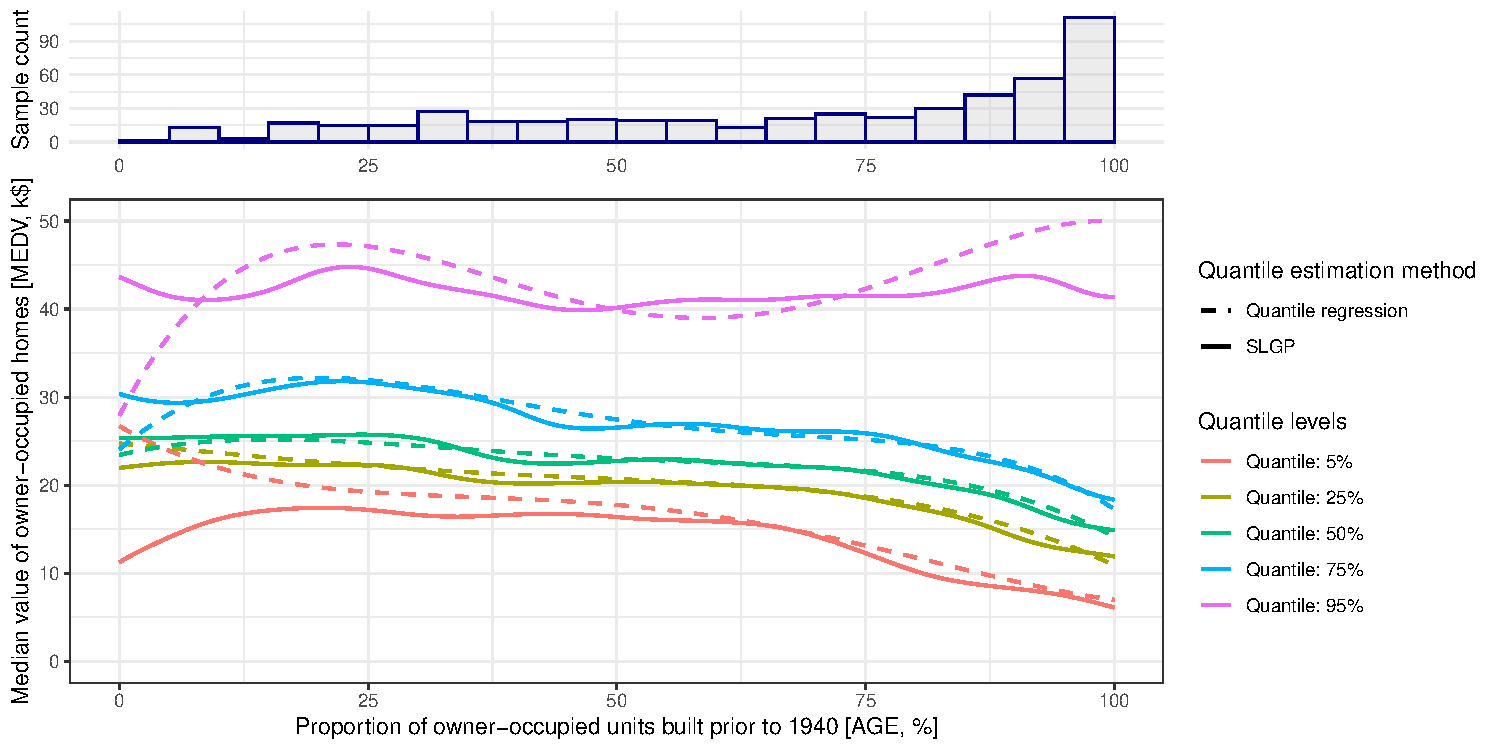
\includegraphics{IntroductionSLGP_files/figure-latex/SLGPMCMCplotQuantiles-1} 

}

\caption{Simultaneous quantile prediction (and associated uncertainty) using a SLGP model}\label{fig:SLGPMCMCplotQuantiles}
\end{figure}

\section{Impact of various parameters on the quality of the estimation}\label{impact-of-various-parameters-on-the-quality-of-the-estimation}

To assess the quality of SLGP-based density field estimation, we first define a reference field using the MAP estimate, which serves as the ground truth. We then generate synthetic data from this reference field and compare different estimation setups to evaluate their impact on accuracy.

For each tested configuration, we compute the estimation error, comparing the inferred density field to the reference field. This allows us to measure the effect of different modeling choices. We investigate the impact of the following factors:

\begin{itemize}
\tightlist
\item
  Incorrect hyperparameters: Using suboptimal lengthscale to quantify the effect of poor prior specification.
\item
  Incorrect smoothness assumption: Comparing inference under a Matérn kernel versus an Exponential kernel.
\item
  Data quantity: Evaluating performance when using fewer or more data points, reflecting real-world data availability constraints.
\item
  Number of basis functions: Exploring the trade-off between approximation accuracy and computational efficiency when reducing or increasing the number of basis functions.
  This analysis provides practical insights into how SLGP estimation behaves under different conditions, guiding model selection for real applications.
\end{itemize}

In order to quantify the prediction error for different configurations, we define an Integrated Hellinger distance to measure dissimilarity between two probability density valued fields \(f(x, \cdot)\) and \(f'(x, \cdot)\):

\[
d_{IH}^2(f , f' ) = \frac{1}{2}\int_D \int_T \left( \sqrt{f(\mathbf{v}, u)} - \sqrt{f'(\mathbf{v}, u))}  \right)^2 \,du \,d\mathbf{v}
\]
We first generate 10 different samples from the reference field.

\begin{Shaded}
\begin{Highlighting}[]
\NormalTok{len\_list }\OtherTok{\textless{}{-}} \FunctionTok{c}\NormalTok{(}\FloatTok{0.01}\NormalTok{, }\FloatTok{0.05}\NormalTok{, }\FloatTok{0.15}\NormalTok{, }\FloatTok{0.5}\NormalTok{)}
\NormalTok{n\_list }\OtherTok{\textless{}{-}} \FunctionTok{c}\NormalTok{(}\DecValTok{5}\NormalTok{, }\DecValTok{25}\NormalTok{, }\DecValTok{100}\NormalTok{, }
            \DecValTok{250}\NormalTok{, }\DecValTok{500}\NormalTok{, }\DecValTok{1000}\NormalTok{, }
            \DecValTok{2500}\NormalTok{, }\DecValTok{5000}\NormalTok{, }\DecValTok{10000}\NormalTok{, }
            \DecValTok{25000}\NormalTok{, }\DecValTok{50000}\NormalTok{, }\DecValTok{100000}\NormalTok{)}
\NormalTok{nFreq\_list }\OtherTok{\textless{}{-}} \FunctionTok{c}\NormalTok{(}\DecValTok{10}\NormalTok{, }\DecValTok{50}\NormalTok{, }\DecValTok{100}\NormalTok{, }\DecValTok{200}\NormalTok{, }\DecValTok{500}\NormalTok{)}
\NormalTok{matpar\_list }\OtherTok{\textless{}{-}} \FunctionTok{c}\NormalTok{(}\DecValTok{1}\SpecialCharTok{/}\DecValTok{2}\NormalTok{, }\DecValTok{5}\SpecialCharTok{/}\DecValTok{2}\NormalTok{, }\ConstantTok{Inf}\NormalTok{)}
\NormalTok{rep\_list }\OtherTok{\textless{}{-}} \FunctionTok{seq}\NormalTok{(}\DecValTok{10}\NormalTok{)}


\ControlFlowTok{for}\NormalTok{(i }\ControlFlowTok{in} \FunctionTok{seq}\NormalTok{(}\FunctionTok{max}\NormalTok{(rep\_list)))\{}
\NormalTok{  title }\OtherTok{\textless{}{-}} \FunctionTok{paste0}\NormalTok{(}\StringTok{"./res/samp\_"}\NormalTok{, i, }\StringTok{".Rdata"}\NormalTok{)}
\NormalTok{  samp }\OtherTok{\textless{}{-}} \FunctionTok{data.frame}\NormalTok{()}
  \ControlFlowTok{if}\NormalTok{(}\SpecialCharTok{!}\NormalTok{(}\FunctionTok{file.exists}\NormalTok{(title)))\{}
    \ControlFlowTok{for}\NormalTok{(slice }\ControlFlowTok{in} \FunctionTok{seq}\NormalTok{(}\DecValTok{10}\NormalTok{))\{  }
      \FunctionTok{cat}\NormalTok{(}\StringTok{"Rep"}\NormalTok{, i, }\StringTok{"slice"}\NormalTok{, slice, }\StringTok{"/10}\SpecialCharTok{\textbackslash{}n}\StringTok{"}\NormalTok{)}
      \FunctionTok{set.seed}\NormalTok{(i}\SpecialCharTok{*}\DecValTok{1000}\SpecialCharTok{*}\NormalTok{slice)}
\NormalTok{      newX }\OtherTok{\textless{}{-}} \FunctionTok{data.frame}\NormalTok{(}\AttributeTok{age=}\FunctionTok{runif}\NormalTok{(}\FunctionTok{max}\NormalTok{(n\_list)}\SpecialCharTok{/}\DecValTok{10}\NormalTok{, range\_x[}\DecValTok{1}\NormalTok{], range\_x[}\DecValTok{2}\NormalTok{]))}
\NormalTok{      temp }\OtherTok{\textless{}{-}} \FunctionTok{sampleSLGP}\NormalTok{(modelMAP, }
                         \AttributeTok{newX =}\NormalTok{ newX, }
                         \AttributeTok{n=}\DecValTok{1}\NormalTok{, }
                         \AttributeTok{interpolateBasisFun =} \StringTok{"WNN"}\NormalTok{)}
\NormalTok{      samp }\OtherTok{\textless{}{-}} \FunctionTok{rbind}\NormalTok{(samp, temp)}
\NormalTok{    \}}
    \FunctionTok{save}\NormalTok{(samp, }\AttributeTok{file=}\NormalTok{title)}
    \FunctionTok{gc}\NormalTok{()}
    
    
\NormalTok{  \}}
\NormalTok{\}}
\end{Highlighting}
\end{Shaded}

And then run the density estimations with different parameters on these samples.

\begin{Shaded}
\begin{Highlighting}[]
\NormalTok{dfGrid }\OtherTok{\textless{}{-}} \FunctionTok{data.frame}\NormalTok{(}\FunctionTok{expand.grid}\NormalTok{(}\FunctionTok{seq}\NormalTok{(range\_x[}\DecValTok{1}\NormalTok{], range\_x[}\DecValTok{2}\NormalTok{],, }\DecValTok{101}\NormalTok{), }
                                 \FunctionTok{seq}\NormalTok{(range\_response[}\DecValTok{1}\NormalTok{], range\_response[}\DecValTok{2}\NormalTok{],, }\DecValTok{101}\NormalTok{)))}
\FunctionTok{colnames}\NormalTok{(dfGrid) }\OtherTok{\textless{}{-}} \FunctionTok{c}\NormalTok{(}\StringTok{"age"}\NormalTok{, }\StringTok{"medv"}\NormalTok{)}
\NormalTok{predRef }\OtherTok{\textless{}{-}} \FunctionTok{predictSLGP\_newNode}\NormalTok{(}\AttributeTok{SLGPmodel=}\NormalTok{modelMAP,}
                               \AttributeTok{newNodes =}\NormalTok{ dfGrid)}

\ControlFlowTok{for}\NormalTok{(i }\ControlFlowTok{in} \FunctionTok{seq}\NormalTok{(}\FunctionTok{max}\NormalTok{(rep\_list)))\{}
  \FunctionTok{set.seed}\NormalTok{(i)}
\NormalTok{  title }\OtherTok{\textless{}{-}} \FunctionTok{paste0}\NormalTok{(}\StringTok{"./res/samp\_"}\NormalTok{, i, }\StringTok{".Rdata"}\NormalTok{)}
  \FunctionTok{load}\NormalTok{(}\AttributeTok{file=}\NormalTok{title)}
  \ControlFlowTok{for}\NormalTok{(matpar }\ControlFlowTok{in}\NormalTok{ matpar\_list)\{}
    \ControlFlowTok{for}\NormalTok{(nFreq }\ControlFlowTok{in}\NormalTok{ nFreq\_list)\{}
\NormalTok{      title2 }\OtherTok{\textless{}{-}} \FunctionTok{paste0}\NormalTok{(}\StringTok{"./res/SLGP\_Mat\_"}\NormalTok{, matpar}\SpecialCharTok{*}\DecValTok{2}\NormalTok{, }
                       \StringTok{"half\_nFreq\_"}\NormalTok{, nFreq,}
                       \StringTok{"\_rep\_"}\NormalTok{, i, }\StringTok{".Rdata"}\NormalTok{)}
      \ControlFlowTok{if}\NormalTok{(}\SpecialCharTok{!}\FunctionTok{file.exists}\NormalTok{(title2))\{}
\NormalTok{        modelCurrent }\OtherTok{\textless{}{-}} \FunctionTok{slgp}\NormalTok{(medv}\SpecialCharTok{\textasciitilde{}}\NormalTok{age, }
                             \AttributeTok{data=}\NormalTok{samp[}\DecValTok{1}\SpecialCharTok{:}\DecValTok{5}\NormalTok{, ],}
                             \AttributeTok{method=}\StringTok{"none"}\NormalTok{, }
                             \AttributeTok{basisFunctionsUsed =} \StringTok{"RFF"}\NormalTok{,}
                             \AttributeTok{interpolateBasisFun=}\StringTok{"WNN"}\NormalTok{, }
                             \AttributeTok{sigmaEstimationMethod =} \StringTok{"heuristic"}\NormalTok{, }
                             \AttributeTok{predictorsLower=} \FunctionTok{c}\NormalTok{(range\_x[}\DecValTok{1}\NormalTok{]),}
                             \AttributeTok{predictorsUpper=} \FunctionTok{c}\NormalTok{(range\_x[}\DecValTok{2}\NormalTok{]),}
                             \AttributeTok{responseRange=}\NormalTok{ range\_response,}
                             \AttributeTok{opts\_BasisFun =} \FunctionTok{list}\NormalTok{(}\AttributeTok{nFreq=}\NormalTok{nFreq,}
                                                  \AttributeTok{MatParam=}\NormalTok{matpar),}
                             \AttributeTok{seed=}\NormalTok{i)}
        \FunctionTok{save}\NormalTok{(modelCurrent, }\AttributeTok{file=}\NormalTok{title2)}
        \FunctionTok{cat}\NormalTok{(}\StringTok{"Created and saved model "}\NormalTok{, title2, }\StringTok{"}\SpecialCharTok{\textbackslash{}n}\StringTok{"}\NormalTok{)}
\NormalTok{      \}}\ControlFlowTok{else}\NormalTok{\{}
        \FunctionTok{load}\NormalTok{(title2)}
\NormalTok{      \}}
      \ControlFlowTok{for}\NormalTok{(len }\ControlFlowTok{in}\NormalTok{ len\_list)\{}
\NormalTok{        title3 }\OtherTok{\textless{}{-}} \FunctionTok{paste0}\NormalTok{(}\StringTok{"./res/Mat\_"}\NormalTok{, matpar}\SpecialCharTok{*}\DecValTok{2}\NormalTok{, }
                         \StringTok{"half\_nFreq\_"}\NormalTok{, nFreq,}
                         \StringTok{"\_len\_"}\NormalTok{, len}\SpecialCharTok{*}\DecValTok{100}\NormalTok{, }\StringTok{"\%"}\NormalTok{,}
                         \StringTok{"\_rep\_"}\NormalTok{, i, }\StringTok{".Rdata"}\NormalTok{)}
\NormalTok{        modelCurrent}\SpecialCharTok{@}\NormalTok{hyperparams}\SpecialCharTok{$}\NormalTok{lengthscale }\OtherTok{\textless{}{-}} \FunctionTok{c}\NormalTok{(len, len)}
        \ControlFlowTok{if}\NormalTok{(}\SpecialCharTok{!}\FunctionTok{file.exists}\NormalTok{(title3) }\SpecialCharTok{|}\NormalTok{ i}\SpecialCharTok{==}\DecValTok{1} \SpecialCharTok{\&}\NormalTok{ nFreq}\SpecialCharTok{==}\DecValTok{100}\NormalTok{)\{}
\NormalTok{          dH\_list }\OtherTok{\textless{}{-}} \FunctionTok{rep}\NormalTok{(}\ConstantTok{NA}\NormalTok{, }\FunctionTok{length}\NormalTok{(n\_list))}
          \ControlFlowTok{for}\NormalTok{(j }\ControlFlowTok{in} \FunctionTok{seq\_along}\NormalTok{(n\_list))\{}
            \FunctionTok{cat}\NormalTok{(}\StringTok{"."}\NormalTok{)}
\NormalTok{            n }\OtherTok{\textless{}{-}}\NormalTok{ n\_list[j]}
\NormalTok{            modelCurrent }\OtherTok{\textless{}{-}} \FunctionTok{retrainSLGP}\NormalTok{(}\AttributeTok{SLGPmodel=}\NormalTok{modelCurrent, }
                                        \AttributeTok{newdata =}\NormalTok{ samp[}\DecValTok{1}\SpecialCharTok{:}\NormalTok{n, ], }
                                        \AttributeTok{method=}\StringTok{"MAP"}\NormalTok{)}
\NormalTok{            predTemp }\OtherTok{\textless{}{-}} \FunctionTok{predictSLGP\_newNode}\NormalTok{(}\AttributeTok{SLGPmodel=}\NormalTok{modelCurrent,}
                                            \AttributeTok{newNodes =}\NormalTok{ dfGrid)}
\NormalTok{            dH }\OtherTok{\textless{}{-}} \FunctionTok{sqrt}\NormalTok{(}\FunctionTok{mean}\NormalTok{((}\FunctionTok{sqrt}\NormalTok{(predRef}\SpecialCharTok{$}\NormalTok{pdf\_1)}\SpecialCharTok{{-}}\FunctionTok{sqrt}\NormalTok{(predTemp}\SpecialCharTok{$}\NormalTok{pdf\_1))}\SpecialCharTok{\^{}}\DecValTok{2}\NormalTok{)}\SpecialCharTok{*}
                         \FunctionTok{diff}\NormalTok{(range\_x)}\SpecialCharTok{*}\FunctionTok{diff}\NormalTok{(range\_response))}
\NormalTok{            dH\_list[j]  }\OtherTok{\textless{}{-}}\NormalTok{ dH}
            \ControlFlowTok{if}\NormalTok{(i}\SpecialCharTok{==}\DecValTok{1} \SpecialCharTok{\&}\NormalTok{ nFreq}\SpecialCharTok{==}\DecValTok{100} \SpecialCharTok{\&}\NormalTok{ n}\SpecialCharTok{==}\DecValTok{100}\NormalTok{)\{}
\NormalTok{              mod1 }\OtherTok{\textless{}{-}}\NormalTok{ modelCurrent}
\NormalTok{            \}}
            \ControlFlowTok{if}\NormalTok{(i}\SpecialCharTok{==}\DecValTok{1} \SpecialCharTok{\&}\NormalTok{ nFreq}\SpecialCharTok{==}\DecValTok{100} \SpecialCharTok{\&}\NormalTok{ n}\SpecialCharTok{==}\DecValTok{10000}\NormalTok{)\{}
\NormalTok{              mod2 }\OtherTok{\textless{}{-}}\NormalTok{ modelCurrent}
\NormalTok{            \}}
\NormalTok{          \}}
          \ControlFlowTok{if}\NormalTok{(i}\SpecialCharTok{==}\DecValTok{1} \SpecialCharTok{\&}\NormalTok{ nFreq}\SpecialCharTok{==}\DecValTok{100}\NormalTok{)\{}
            \FunctionTok{save}\NormalTok{(dH\_list, mod1, mod2, }\AttributeTok{file=}\NormalTok{title3)}
\NormalTok{          \}}\ControlFlowTok{else}\NormalTok{\{}
            \FunctionTok{save}\NormalTok{(dH\_list, }\AttributeTok{file=}\NormalTok{title3)}
\NormalTok{          \}}
          \FunctionTok{cat}\NormalTok{(}\StringTok{"Did "}\NormalTok{, title3, }\StringTok{"}\SpecialCharTok{\textbackslash{}n}\StringTok{"}\NormalTok{)}
          \FunctionTok{gc}\NormalTok{()}
\NormalTok{        \}}
\NormalTok{      \}}
\NormalTok{    \}}
\NormalTok{  \}}
\NormalTok{\}}
\end{Highlighting}
\end{Shaded}

we concatenate the results and are ready to visualise them.

\begin{Shaded}
\begin{Highlighting}[]
\NormalTok{df\_res }\OtherTok{\textless{}{-}} \FunctionTok{data.frame}\NormalTok{()}

\ControlFlowTok{for}\NormalTok{(i }\ControlFlowTok{in} \FunctionTok{seq}\NormalTok{(}\FunctionTok{max}\NormalTok{(rep\_list)))\{}
  \ControlFlowTok{for}\NormalTok{(matpar }\ControlFlowTok{in}\NormalTok{ matpar\_list)\{}
    \ControlFlowTok{for}\NormalTok{(nFreq }\ControlFlowTok{in}\NormalTok{ nFreq\_list)\{}
      \ControlFlowTok{for}\NormalTok{(len }\ControlFlowTok{in}\NormalTok{ len\_list)\{}
\NormalTok{        title3 }\OtherTok{\textless{}{-}} \FunctionTok{paste0}\NormalTok{(}\StringTok{"./res/Mat\_"}\NormalTok{, matpar}\SpecialCharTok{*}\DecValTok{2}\NormalTok{, }
                         \StringTok{"half\_nFreq\_"}\NormalTok{, nFreq,}
                         \StringTok{"\_len\_"}\NormalTok{, len}\SpecialCharTok{*}\DecValTok{100}\NormalTok{, }\StringTok{"\%"}\NormalTok{,}
                         \StringTok{"\_rep\_"}\NormalTok{, i, }\StringTok{".Rdata"}\NormalTok{)}
        \ControlFlowTok{if}\NormalTok{(}\FunctionTok{file.exists}\NormalTok{(title3))\{}
          \FunctionTok{load}\NormalTok{(}\AttributeTok{file=}\NormalTok{title3)}
\NormalTok{          temp }\OtherTok{\textless{}{-}} \FunctionTok{data.frame}\NormalTok{(}\AttributeTok{matpar=}\NormalTok{matpar,}
                             \AttributeTok{nFreq=}\NormalTok{nFreq,}
                             \AttributeTok{len=}\NormalTok{len,}
                             \AttributeTok{n=}\NormalTok{n\_list, }
                             \AttributeTok{dH=}\NormalTok{dH\_list, }
                             \AttributeTok{rep=}\NormalTok{i)}
\NormalTok{          df\_res }\OtherTok{\textless{}{-}} \FunctionTok{rbind}\NormalTok{(df\_res, temp)}
\NormalTok{        \}}
\NormalTok{      \}}
\NormalTok{    \}}
\NormalTok{  \}}
\NormalTok{\}}
\end{Highlighting}
\end{Shaded}

When the lengthscale is too small, the estimation fails to generalize effectively, leading to poor density reconstruction.

\begin{Shaded}
\begin{Highlighting}[]
\NormalTok{df\_res\_plot }\OtherTok{\textless{}{-}}\NormalTok{ df\_res }\SpecialCharTok{\%\textgreater{}\%}
  \FunctionTok{group\_by}\NormalTok{(matpar, nFreq, len, n)}\SpecialCharTok{\%\textgreater{}\%}
  \FunctionTok{summarise}\NormalTok{(}\AttributeTok{meandH=}\FunctionTok{mean}\NormalTok{(dH),}
            \AttributeTok{q10=}\FunctionTok{quantile}\NormalTok{(dH, }\AttributeTok{probs=}\FloatTok{0.1}\NormalTok{),}
            \AttributeTok{q90=}\FunctionTok{quantile}\NormalTok{(dH, }\AttributeTok{probs=}\FloatTok{0.9}\NormalTok{), }\AttributeTok{.groups=}\StringTok{"keep"}\NormalTok{) }\SpecialCharTok{\%\textgreater{}\%}
  \FunctionTok{ungroup}\NormalTok{()}\SpecialCharTok{\%\textgreater{}\%}
  \FunctionTok{mutate}\NormalTok{(}\AttributeTok{len=}\FunctionTok{paste0}\NormalTok{(}\StringTok{"Lengthscale: "}\NormalTok{, }\DecValTok{100}\SpecialCharTok{*}\NormalTok{len,}
                    \StringTok{"\%}\SpecialCharTok{\textbackslash{}n}\StringTok{ of the range"}\NormalTok{))}\SpecialCharTok{\%\textgreater{}\%}
  \FunctionTok{mutate}\NormalTok{(}\AttributeTok{len=}\FunctionTok{factor}\NormalTok{(len, }\AttributeTok{levels=} \FunctionTok{paste0}\NormalTok{(}\StringTok{"Lengthscale: "}\NormalTok{, }
                                        \FunctionTok{c}\NormalTok{(}\DecValTok{1}\NormalTok{, }\DecValTok{5}\NormalTok{, }\DecValTok{15}\NormalTok{, }\DecValTok{50}\NormalTok{),}
                                        \StringTok{"\%}\SpecialCharTok{\textbackslash{}n}\StringTok{ of the range"}\NormalTok{)))}\SpecialCharTok{\%\textgreater{}\%}
  \FunctionTok{mutate}\NormalTok{(}\AttributeTok{matpar=}\FunctionTok{ifelse}\NormalTok{(}\FunctionTok{is.infinite}\NormalTok{(matpar), }
                       \StringTok{"RFF of Gaussian kernel"}\NormalTok{, }
\NormalTok{                       matpar))}\SpecialCharTok{\%\textgreater{}\%}
  \FunctionTok{mutate}\NormalTok{(}\AttributeTok{matpar=}\FunctionTok{ifelse}\NormalTok{(matpar}\SpecialCharTok{==}\FloatTok{0.5}\NormalTok{, }
                       \StringTok{"RFF of exponential kernel"}\NormalTok{, }
\NormalTok{                       matpar))}\SpecialCharTok{\%\textgreater{}\%}
  \FunctionTok{mutate}\NormalTok{(}\AttributeTok{matpar=}\FunctionTok{ifelse}\NormalTok{(matpar}\SpecialCharTok{==}\FloatTok{2.5}\NormalTok{, }
                       \StringTok{"RFF of Matérn 5/2 kernel"}\NormalTok{, }
\NormalTok{                       matpar))}\SpecialCharTok{\%\textgreater{}\%}
  \FunctionTok{mutate}\NormalTok{(}\AttributeTok{matpar=}\FunctionTok{factor}\NormalTok{(matpar, }\AttributeTok{levels=} \FunctionTok{paste0}\NormalTok{(}\StringTok{"RFF of "}\NormalTok{,}
                                              \FunctionTok{c}\NormalTok{(}\StringTok{"exponential"}\NormalTok{,}
                                                \StringTok{"Matérn 5/2"}\NormalTok{,}
                                                \StringTok{"Gaussian"}\NormalTok{),}
                                              \StringTok{" kernel"}\NormalTok{)))}\SpecialCharTok{\%\textgreater{}\%}
  \FunctionTok{data.frame}\NormalTok{()}
\NormalTok{df\_res\_plot }\SpecialCharTok{\%\textgreater{}\%}
  \FunctionTok{filter}\NormalTok{(}\FunctionTok{as.numeric}\NormalTok{(len) }\SpecialCharTok{==}\DecValTok{1}\NormalTok{ ) }\SpecialCharTok{\%\textgreater{}\%}
  \FunctionTok{ggplot}\NormalTok{(}\FunctionTok{aes}\NormalTok{(}\AttributeTok{x=}\NormalTok{n, }\AttributeTok{group=}\NormalTok{nFreq, }
             \AttributeTok{col=}\FunctionTok{as.factor}\NormalTok{(nFreq), }\AttributeTok{fill=}\FunctionTok{as.factor}\NormalTok{(nFreq)))}\SpecialCharTok{+}
  \FunctionTok{geom\_ribbon}\NormalTok{(}\AttributeTok{mapping=}\FunctionTok{aes}\NormalTok{(}\AttributeTok{ymin =}\NormalTok{ q10, }\AttributeTok{ymax=}\NormalTok{q90), }\AttributeTok{alpha=}\FloatTok{0.1}\NormalTok{)}\SpecialCharTok{+}
  \FunctionTok{geom\_line}\NormalTok{(}\AttributeTok{mapping=} \FunctionTok{aes}\NormalTok{(}\AttributeTok{y=}\NormalTok{meandH))}\SpecialCharTok{+}
  \FunctionTok{theme\_bw}\NormalTok{()}\SpecialCharTok{+}
  \FunctionTok{facet\_grid}\NormalTok{(len}\SpecialCharTok{\textasciitilde{}}\NormalTok{matpar)}\SpecialCharTok{+}
  \FunctionTok{scale\_x\_log10}\NormalTok{()}\SpecialCharTok{+}
  \FunctionTok{scale\_y\_log10}\NormalTok{()}\SpecialCharTok{+}
  \FunctionTok{xlab}\NormalTok{(}\StringTok{"Size of the training sample"}\NormalTok{)}\SpecialCharTok{+}
  \FunctionTok{ylab}\NormalTok{(}\StringTok{"Integrated square Hellinger distance"}\NormalTok{)}\SpecialCharTok{+}
  \FunctionTok{labs}\NormalTok{(}\AttributeTok{fill =} \StringTok{"Number of frequencies"}\NormalTok{,}
       \AttributeTok{col=} \StringTok{"Number of frequencies"}\NormalTok{)}\SpecialCharTok{+}
  \FunctionTok{theme}\NormalTok{(}\AttributeTok{legend.direction =} \StringTok{"horizontal"}\NormalTok{, }\AttributeTok{legend.position =} \StringTok{"bottom"}\NormalTok{)}
\end{Highlighting}
\end{Shaded}

\begin{figure}[H]

{\centering 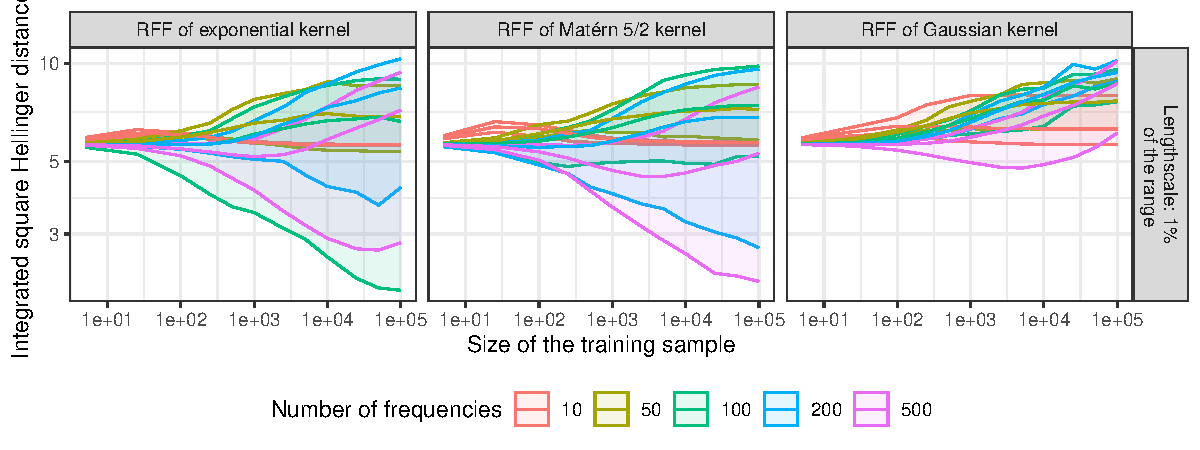
\includegraphics{IntroductionSLGP_files/figure-latex/PlotTooSmallLen-1} 

}

\caption{Integrated square Hellinger distance between reference field and estimated field, when the lengthscale is too small}\label{fig:PlotTooSmallLen}
\end{figure}

Indeed, with such low lengthscale, the model struggles to share information across different regions, the predictive uncertainty remains high even as the amount of data increases. This is reflected in the Integrated Hellinger distance, which does not decrease significantly as more observations are incorporated.

For other, more reasonable values of the lengthscales, we observe more satisfying behaviours:

\begin{Shaded}
\begin{Highlighting}[]

\NormalTok{df\_res\_plot }\SpecialCharTok{\%\textgreater{}\%}
  \FunctionTok{filter}\NormalTok{(}\FunctionTok{as.numeric}\NormalTok{(len) }\SpecialCharTok{!=}\DecValTok{1}\NormalTok{ ) }\SpecialCharTok{\%\textgreater{}\%}
  \FunctionTok{ggplot}\NormalTok{(}\FunctionTok{aes}\NormalTok{(}\AttributeTok{x=}\NormalTok{n, }\AttributeTok{group=}\NormalTok{nFreq, }
             \AttributeTok{col=}\FunctionTok{as.factor}\NormalTok{(nFreq), }\AttributeTok{fill=}\FunctionTok{as.factor}\NormalTok{(nFreq)))}\SpecialCharTok{+}
  \FunctionTok{geom\_ribbon}\NormalTok{(}\AttributeTok{mapping=}\FunctionTok{aes}\NormalTok{(}\AttributeTok{ymin =}\NormalTok{ q10, }\AttributeTok{ymax=}\NormalTok{q90), }\AttributeTok{alpha=}\FloatTok{0.1}\NormalTok{)}\SpecialCharTok{+}
  \FunctionTok{geom\_line}\NormalTok{(}\AttributeTok{mapping=} \FunctionTok{aes}\NormalTok{(}\AttributeTok{y=}\NormalTok{meandH))}\SpecialCharTok{+}
  \FunctionTok{theme\_bw}\NormalTok{()}\SpecialCharTok{+}
  \FunctionTok{facet\_grid}\NormalTok{(len}\SpecialCharTok{\textasciitilde{}}\NormalTok{matpar)}\SpecialCharTok{+}
  \FunctionTok{scale\_x\_log10}\NormalTok{()}\SpecialCharTok{+}
  \FunctionTok{scale\_y\_log10}\NormalTok{()}\SpecialCharTok{+}
  \FunctionTok{xlab}\NormalTok{(}\StringTok{"Size of the training sample"}\NormalTok{)}\SpecialCharTok{+}
  \FunctionTok{ylab}\NormalTok{(}\StringTok{"Integrated square Hellinger distance"}\NormalTok{)}\SpecialCharTok{+}
  \FunctionTok{labs}\NormalTok{(}\AttributeTok{fill =} \StringTok{"Number of frequencies"}\NormalTok{,}
       \AttributeTok{col=} \StringTok{"Number of frequencies"}\NormalTok{)}\SpecialCharTok{+}
  \FunctionTok{theme}\NormalTok{(}\AttributeTok{legend.direction =} \StringTok{"horizontal"}\NormalTok{, }\AttributeTok{legend.position =} \StringTok{"bottom"}\NormalTok{)}
\end{Highlighting}
\end{Shaded}

\begin{figure}[H]

{\centering 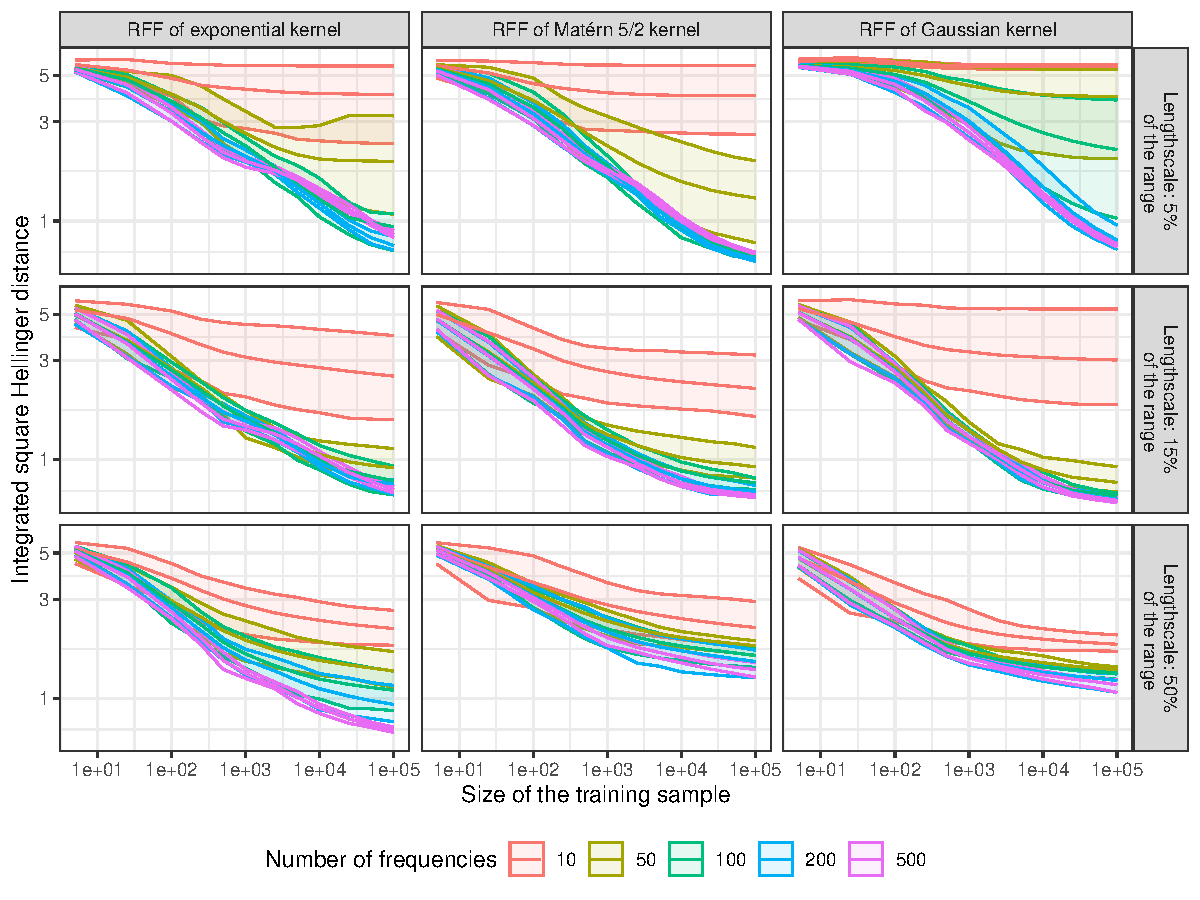
\includegraphics{IntroductionSLGP_files/figure-latex/PlotOtherLen-1} 

}

\caption{Integrated square Hellinger distance between reference field and estimated field, when the lengthscale is reasonably small, correct, and reasonably big}\label{fig:PlotOtherLen}
\end{figure}

\begin{Shaded}
\begin{Highlighting}[]

\NormalTok{df\_res\_plot }\SpecialCharTok{\%\textgreater{}\%}
  \FunctionTok{filter}\NormalTok{(}\FunctionTok{as.numeric}\NormalTok{(len) }\SpecialCharTok{!=}\DecValTok{1}\NormalTok{ ) }\SpecialCharTok{\%\textgreater{}\%}
  \FunctionTok{filter}\NormalTok{(n }\SpecialCharTok{\textgreater{}=}\DecValTok{100}\NormalTok{) }\SpecialCharTok{\%\textgreater{}\%}
  \FunctionTok{ggplot}\NormalTok{(}\FunctionTok{aes}\NormalTok{(}\AttributeTok{x=}\NormalTok{n, }\AttributeTok{group=}\NormalTok{nFreq, }
             \AttributeTok{col=}\FunctionTok{as.factor}\NormalTok{(nFreq), }\AttributeTok{fill=}\FunctionTok{as.factor}\NormalTok{(nFreq)))}\SpecialCharTok{+}
  \FunctionTok{geom\_ribbon}\NormalTok{(}\AttributeTok{mapping=}\FunctionTok{aes}\NormalTok{(}\AttributeTok{ymin =}\NormalTok{ q10, }\AttributeTok{ymax=}\NormalTok{q90), }\AttributeTok{alpha=}\FloatTok{0.1}\NormalTok{)}\SpecialCharTok{+}
  \FunctionTok{geom\_line}\NormalTok{(}\AttributeTok{mapping=} \FunctionTok{aes}\NormalTok{(}\AttributeTok{y=}\NormalTok{meandH))}\SpecialCharTok{+}
  \FunctionTok{theme\_bw}\NormalTok{()}\SpecialCharTok{+}
  \FunctionTok{facet\_grid}\NormalTok{(len}\SpecialCharTok{\textasciitilde{}}\NormalTok{matpar)}\SpecialCharTok{+}
  \FunctionTok{coord\_cartesian}\NormalTok{(}\AttributeTok{ylim=}\FunctionTok{c}\NormalTok{(}\FunctionTok{min}\NormalTok{(df\_res}\SpecialCharTok{$}\NormalTok{dH), }\DecValTok{2}\NormalTok{))}\SpecialCharTok{+}
  \FunctionTok{scale\_x\_log10}\NormalTok{()}\SpecialCharTok{+}
  \FunctionTok{scale\_y\_log10}\NormalTok{()}\SpecialCharTok{+}
  \FunctionTok{xlab}\NormalTok{(}\StringTok{"Size of the training sample"}\NormalTok{)}\SpecialCharTok{+}
  \FunctionTok{ylab}\NormalTok{(}\StringTok{"Integrated square Hellinger distance"}\NormalTok{)}\SpecialCharTok{+}
  \FunctionTok{labs}\NormalTok{(}\AttributeTok{fill =} \StringTok{"Number of frequencies"}\NormalTok{,}
       \AttributeTok{col=} \StringTok{"Number of frequencies"}\NormalTok{)}\SpecialCharTok{+}
  \FunctionTok{theme}\NormalTok{(}\AttributeTok{legend.direction =} \StringTok{"horizontal"}\NormalTok{, }\AttributeTok{legend.position =} \StringTok{"bottom"}\NormalTok{)}
\end{Highlighting}
\end{Shaded}

\begin{figure}[H]

{\centering 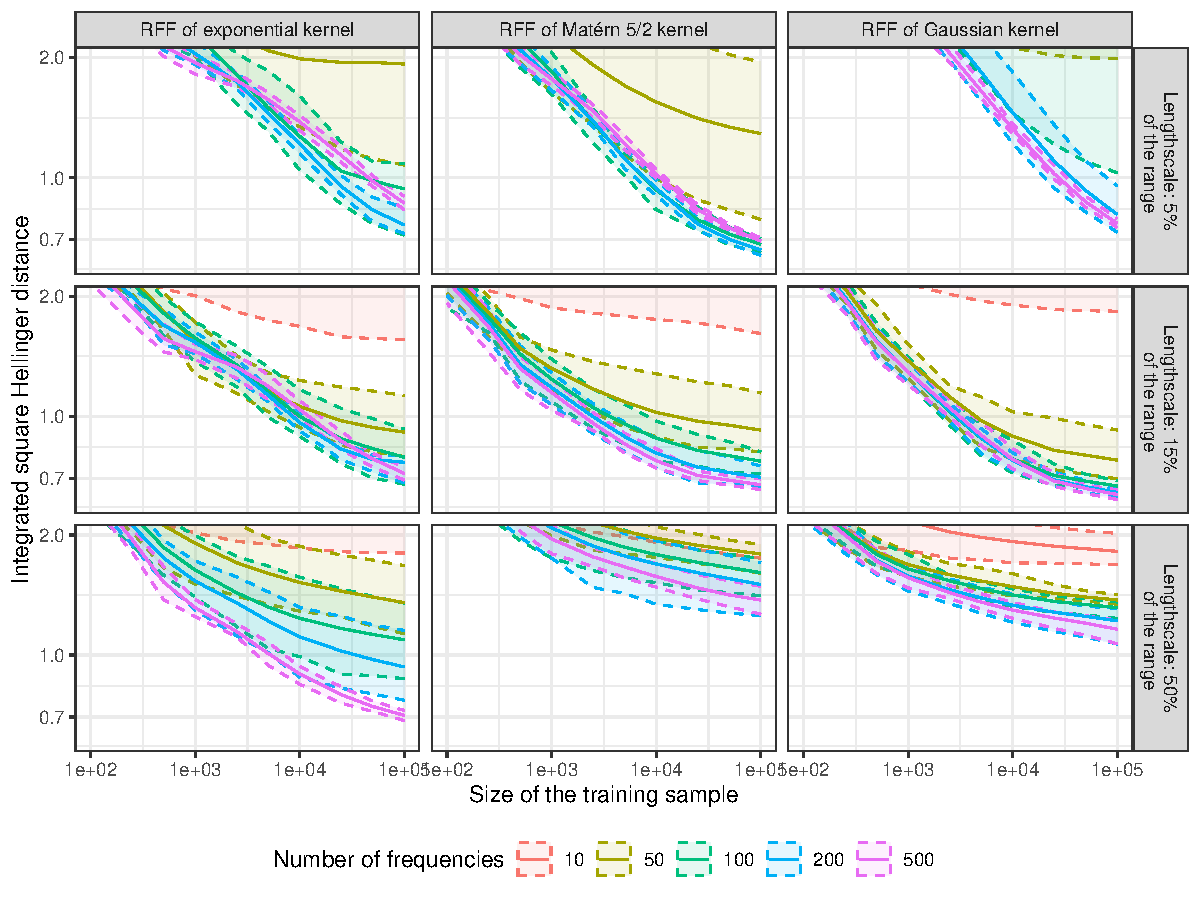
\includegraphics{IntroductionSLGP_files/figure-latex/PlotOtherLen2-1} 

}

\caption{Integrated square Hellinger distance between reference field and estimated field, when the lengthscale is reasonably small, correct, and reasonably big. (Same results, different scale)}\label{fig:PlotOtherLen2}
\end{figure}

Indeed, one notices that higher number of frequencies (i.e.~of basis functions) increases the performances of the mode, until the well-specified setting (200 frequencies) is reached.

As observed qualitatively in the MAP section, models that are too smooth (wrong kernel assumptions and/or wrong lengthscale), struggle to capture fine-scale elements.

  \bibliography{references.bib}

\end{document}
